\documentclass[oneside]{amsbook}
\usepackage[T1]{fontenc}
\usepackage[utf8]{inputenc}
\usepackage[active]{srcltx}
\usepackage{float}
\usepackage{textcomp}
\usepackage{amsthm}
\usepackage{graphicx}
\usepackage{setspace}
\usepackage{imakeidx}
\usepackage{subscript}
\usepackage [italian]{babel}
\usepackage{hyperref}
\usepackage{amsmath}
\usepackage{amsfonts}
\usepackage{amssymb}
\usepackage{titlepic}


\makeindex
\makeatletter
\providecommand{\tabularnewline}{\\}
%%%%%%%%%%%%%%%%%%%%%%%%%%%%%% Textclass specific LaTeX commands.
\numberwithin{section}{chapter}
%\numberwithin{table} {subsection}
\numberwithin{equation}{section}
\numberwithin{figure}{section}
\makeatother
\begin{document}
\begin{titlepage}
\title{Riassunti e approfondimenti di\\ \textit{\Huge Chimica Teorica e Computazionale}}
\titlepic{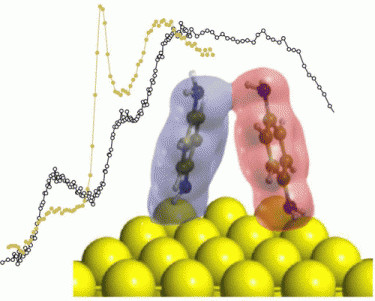
\includegraphics[scale=0.6]{chim}}

\end{titlepage}
\maketitle

 A cura di: \textit{\Large swannyyy}
\begin{figure}
{\small Quest'opera è stata rilasciata con licenza Creative Commons Attribuzione - Non commerciale 3.0 Italia. Per leggere una copia della licenza visita il sito web http://creativecommons.org/licenses/by-nc/3.0/it/ o spedisci una lettera a Creative Commons, PO Box 1866, Mountain View, CA 94042, USA.}
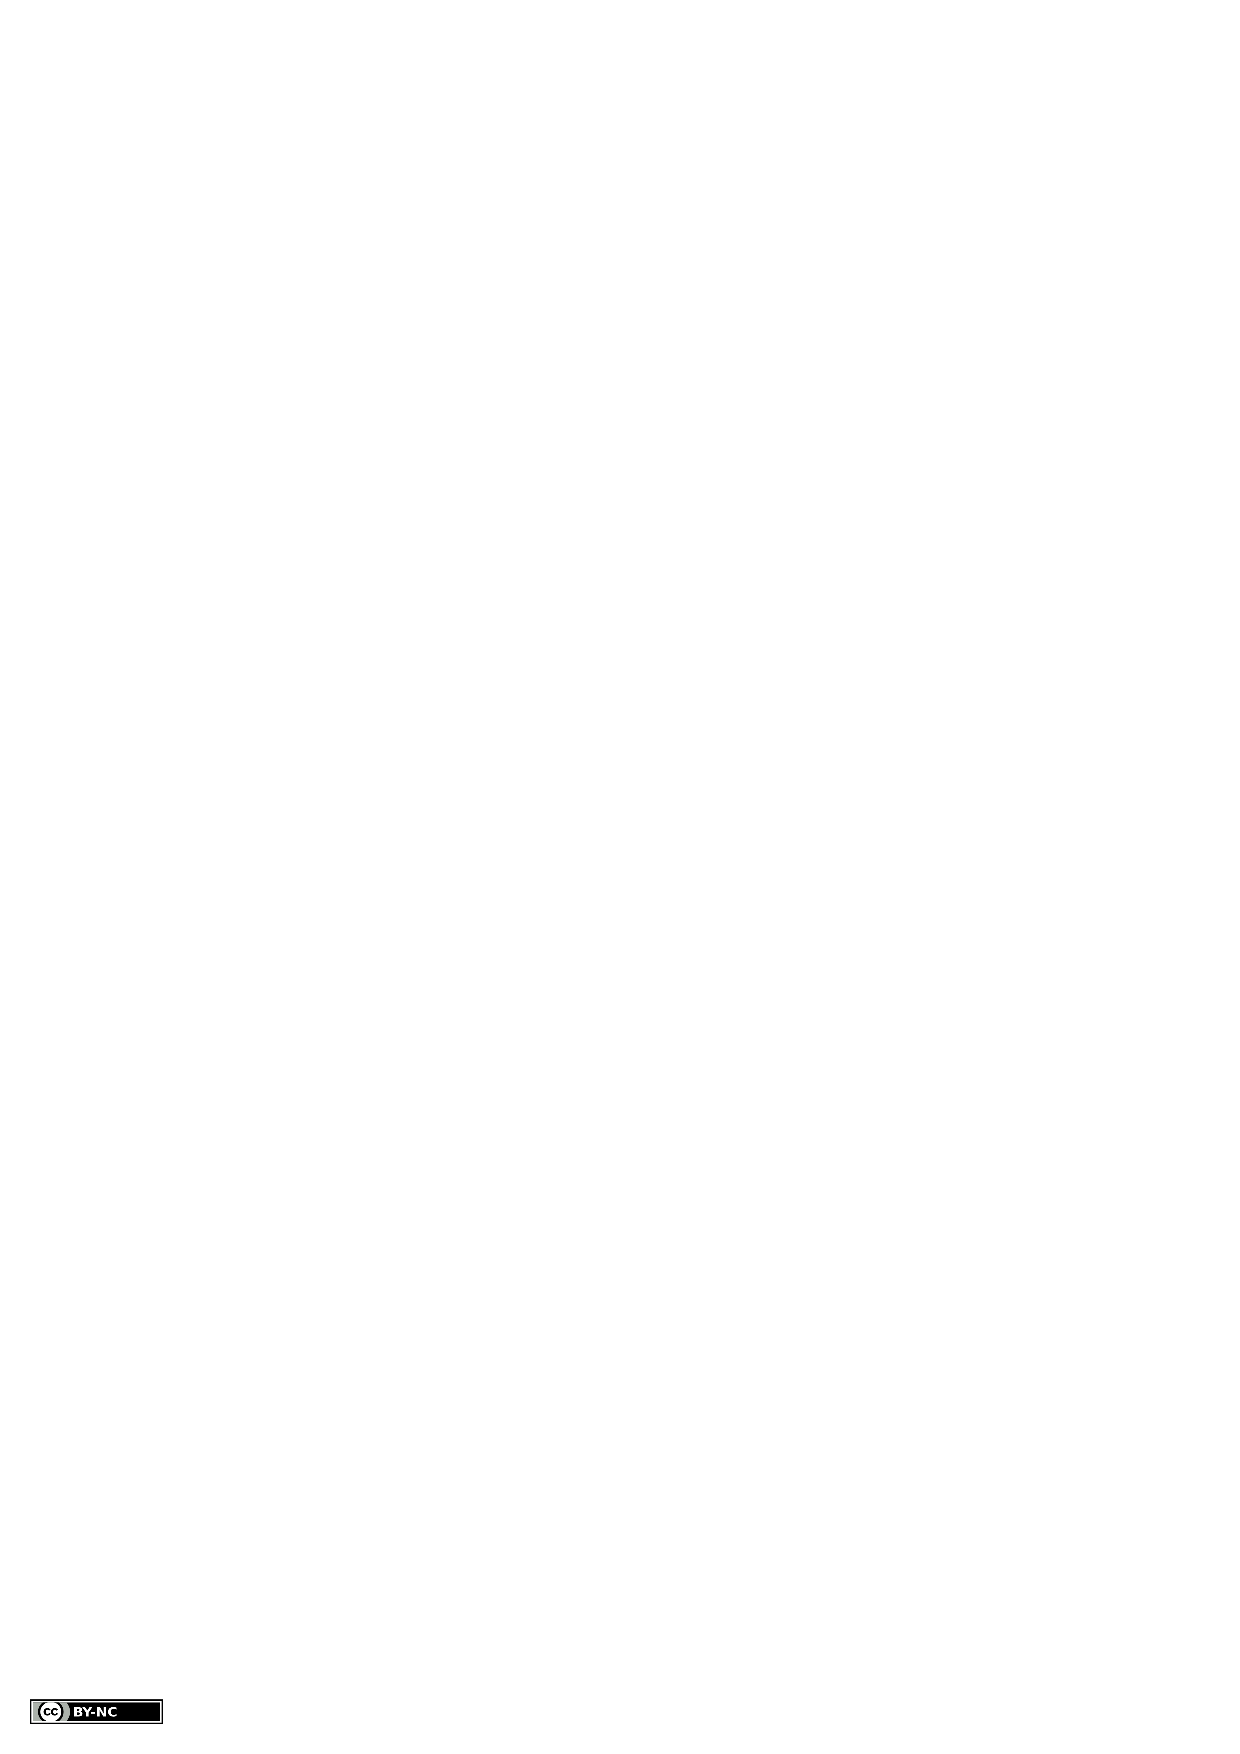
\includegraphics[scale=1.0]{licenza}
\end{figure}

\tableofcontents{}

\chapter*{Cosa non studiare?}
Il presente testo non deve essere considerato sostitutivo degli appunti presi in classe o delle dispense fornite dai professori, sebbene tutti gli argomenti trattati durante i corsi siano inclusi. La motivazione risiede negli obiettivi che quest'opera si presupponeva di raggiungere; infatti questo testo nasce dall'esigenza personale dell'autore di scrivere in un'unica raccolta di concetti tutte le nozioni relative la chimica teorica. Per puro interesse personale alcune parti sono state ampliate rispetto il programma dei corsi mentre altre sono state riassunte non perché meno importanti o di limitato interesse ma per far fronte a esigenze di studio particolari. Data la non generalità del organizzazione della conoscenza operata in quest'opera, in seguito a una serie di confronti con il titolare del corso di Computazionale, ho deciso di riportare di seguito una breve lista dei paragrafi di approfondimento che non vengono trattati nel ambito del corso di \emph{Chimica Computazionale}.
\begin{itemize}
\item Il paragrafo \ref{ee2};
\item Il paragrafo \ref{ee3};
\item Il paragrafo \ref{densr};
\item Il capitolo \ref{semi};
\item Tutti i capitoli afferenti alla parte \ref{p3}.
\end{itemize}
Alcuni lettori potrebbero domandarsi perché la parte \ref{p3} sia stata inserita. Le motivazioni principali sono: per completezza dell'opera, in quanto un elenco di metodi senza un esempio di loro applicazione resta un mero elenco; e perché lo studio integrale della parte \ref{p3} porta alla preparazione del primo esonero del corso di \emph{Complementi di Scienze dei Materiali Computazionali}.
Gli argomenti trattati in quest'opera sono comunque tratti dall'organizzazione dei corsi svoltasi tra il 2017 e il 2019. Pertanto ogni modifica successiva agli argomenti non viene presa in considerazione.
L'opera è tuttora incompleta, e lo sarà a tempo indefinito, infatti nell'idea originale essa avrebbe dovuto contenere un ulteriore capitolo finale di riassunto degli argomenti trattati nel corso \emph{Modellistica molecolare}. Per ragioni legate alla mia organizzazione del percorso di laurea quando ho studiato per tale esame non mi sono preoccupato di trascrivere la conoscenza acquisita. Inoltre i continui aggiornamenti degli argomenti affrontati nei corsi non potranno, inevitabilmente, essere inclusi.  Pertanto chiunque voglia contribuire e desideri quindi occuparsi del capitolo finale e dell'aggiornamento di questo testo è libero di farlo. Tutto il materiale necessario alla modifica del presente file sarà reso gratuito sul sito git-hub al link \url{https://github.com/swannyyy/Appunti_Chimica_Computazionale}.
\chapter{Superficie di energia potenziale (PES) e sua analisi}
\section{Che cos'è la PES?}
L'\index{energia !potenziale}energia potenziale che possiede una molecola in un suo qualsiasi stato, sia esso fondamentale o eccitato, è l'unica caratteristica che definisce totalmente qualsiasi tipo di reattività. Si immagini che la molecola sia una pallina in cima a una collina circondata da valli più o meno alte, altre colline e passi tra le valli. La via che la pallina percorrerà preferenzialmente è determinata esclusivamente dalla facilità con cui essa potrà cadere attraverso il panorama appena descritto. In perfetta analogia con questa pallina, le molecole si ritrovano in un "panorama montuoso" a diverse energie potenziali (altitudini, ricordando che $U=mgh$, con $h=altezza$); quindi soltanto uno dei possibili percorsi di energia potenziale sarà il favorito in determinate condizioni. A questo punto della trattazione è bene considerare il carattere più generale di questa teoria; infatti dove, fin'ora, si è parlato di molecola, si può, e si dovrebbe parlare di \emph{sistema} nella sua accezione più termodinamica. 
Con il termine \emph{sistema} si intende infatti sia qualsiasi molecola, sia qualsiasi \emph{insieme di molecole}. Questa precisazione è fondamentale, in quanto la maggior parte dei calcoli che vengono svolti al giorno d'oggi in ambito molecolare coinvolgono più molecole e si prefiggono il compito di comprenderne la reattività. In quest'ottica la nostra pallina non sarà più una singola molecola, bensì una rappresentazione dell'insieme di molecole all'inizio di una reazione ovvero i \emph{reagenti}; il percorso più facile costituirà la \emph{coordinata di reazione}; e la valle dove la pallina terminerà la sua corsa sarà l'insieme di molecole finale ovvero i \emph{prodotti}.

\begin{figure}[H]
\centering
\caption{A sinistra un rilievo topografico della California orientale. A destra la tipica superficie di energia potenziale di un sistema molecolare.}\label{pesconf}
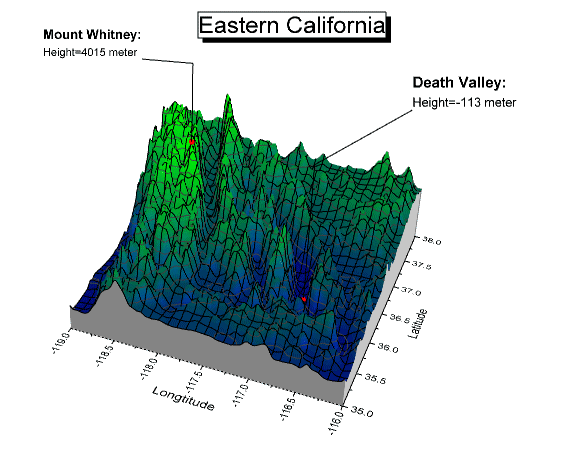
\includegraphics[scale=1.2]{PES_California}
\hfil
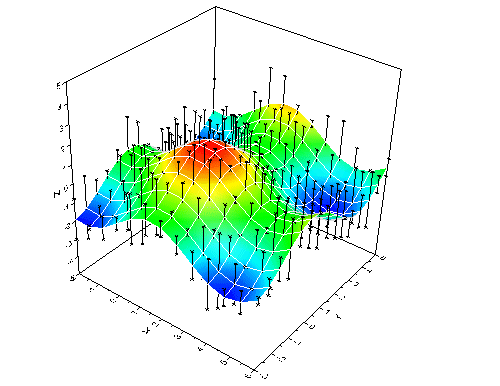
\includegraphics[scale=1.2]{PES_molecola}
\end{figure}

\section{L'energia potenziale è funzione della geometria molecolare}
Lo studio della superficie di energia potenziale nella razionalizzazione della reattività chimica è di fondamentale importanza: risulta cruciale, quindi, capire quali siano le dipendenze intrinseche tra la natura della molecola e l'energia potenziale a essa associata.
\`E noto che data una determinata \emph{geometria} sia possibile calcolare un'energia potenziale. Tuttavia, ciò risulta vero solo se si considera applicabile al sistema in esame, l'approssimazione di \emph{Born-Oppenheimer}. Applicare tale approssimazione, infatti, significa "separare il moto dei nuclei da quello degli elettroni" e considerare i nuclei sostanzialmente fermi rispetto agli elettroni. \`E possibile, quindi, calcolare l'energia associata a un insieme di posizioni nucleari fisse (\emph{geometria molecolare}) rappresentabili in termini di coordinate cartesiane come si vede in Eq.\ref{PesEq}.
\begin{equation}
\label{PesEq}
E_{PES}=E(x_1,y_1,z_1;x_2,y_2,z_2;...;x_N,y_N,z_N)
\end{equation}
Scrivendo la forma funzionale della PES in questi termini, risulta che essa esisterà in uno spazio a $3N$ dimensioni dove $N$ è il numero degli atomi. Questa enorme dimensionalità può essere ridotta in due modi:
\begin{enumerate}
\item Fissando l'origine nel \emph{centro di massa} della molecola;
\item Allineando i \emph{momenti d'inerzia principali} della molecole con gli assi $x$, $y$ e $z$.
\end{enumerate}
Questi 2 piccoli accorgimenti permettono di eliminare 3 coordinate dovute ai 3 gradi di libertà transazionali (1) e 3 coordinanate associate ai gradi di libertà rotazionali (2). Alla fine di questo procedimento l'energia potenziale sarà funzione di sole $3N-6$ coordinate.

\subsection{Un'altra definizione della geometria}
Le coordinate cartesiane forniscono un'ottima rappresentazione matematica della geometria; tuttavia risulta difficile costruire un tale sistema di coordinate basandosi esclusivamente su considerazioni chimiche. Per ovviare a questo problema è stato costruito un nuovo sistema di coordinate, dette \emph{interne}, con le quali vengono specificate distanze di legame, angoli di legame e angoli diedri della molecola. Tale sistema risulta più coerente con il comune senso chimico e rende estremamente più facile costruire una geometria. Con l'avvento di interfacce grafiche più elaborate, nei comuni programmi per calcoli molecolari, la necessità di questo sistema è venuta meno. Infatti, ora è possibile costruire svariate geometrie molecolari con semplici programmi grafici come GaussView o Avogadro.\\
\`E interessante notare che, facendo uso di differenti sistemi di coordinate,la sagoma della superificie di potenziale cambia, mentre i rapporti tra i differenti stati che il sistema può assumere rimangono invariati. Ciò significa che è indifferente quale sistema di coordinate si usi, (\emph{cartesiane} o \emph{interne}), perché il risultato rimarrà lo stesso.
\section{I punti stazionari della PES definiscono lo stato del sistema}
La più diretta \emph{interpretazione chimica} della PES consiste nella razionalizzazione della reattività chimica attraverso lo studio degli avvallamenti e delle alture che costituiscono la superficie di energia potenziale.
\subsection{Geometrie di equilibrio}
Le tipiche \emph{geometrie di equilibrio} che si studiano nell'ottica di razionalizzare la reattività sono \emph{reagenti} e \emph{prodotti}.
Entrambi questi concetti sono comunemente utilizzati in ogni ambito della chimica sperimentale e sintetica ma dal punto di vista teorico essi costituiscono un ottimo esempio di \emph{sistema in equilibrio}. Quando un sistema si trova in condizioni di \emph{equilibrio termodinamico} esso costituisce un minimo nella superficie di energia potenziale. Tale minimo può essere efficaciemente descritto da diverse forme funzionali a seconda del potenziale scelto come approssimazione.
L'allargamento del minimo dà una misura della flessibilità del sistema chimico studiato. Ricordando che l'energia è funzione della geometria, a diverse energie corrispondono diverse strutture, quindi punti di minimo poco localizzati potranno spaziare tra geometrie molto variegate.

\begin{figure}[H]
\centering
\caption{ A sinistra: figura di potenziale che descrive il percorso di collegamento tra i punti di minimo dei reagenti e dei prodotti. A destra: paragone tra due diverse forme funzionali atte a descrivere l'energia potenziale di un punto di minimo.}\label{rep}
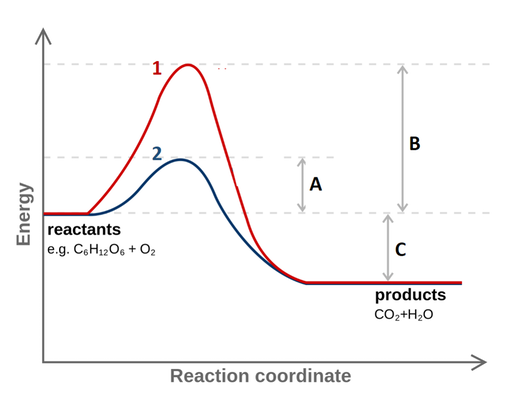
\includegraphics[scale=0.3]{rep}
\hfil
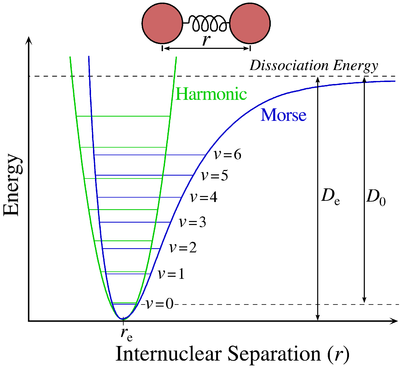
\includegraphics[scale=0.3]{pot}
\end{figure}

\subsection{Strutture di transizione}
Le \emph{strutture di transizione} costituiscono un concetto tipico della chimica organica sintetica, nella quale ricoprono il ruolo di "\emph{entità astratta}" spesso etichettata come \emph{non conoscibile}.
Nell'ambito della chimica teorica gli stati di transizione ricoprono un ruolo fondamentale, infatti permettono di calcolare le energie di attivazione, e conseguentemente, tutti i parametri  termodinamici e cinetici della reazione analizzata.
Gli stati di transizione sono rapresentati sulla superficie di energia potenziale da \emph{punti di sella}.

\begin{figure}[H]
\centering
\caption{ In questa figura viene identificato come Transition Structure A il punto di sella che collega i prodotti ai reagenti.}\label{pes}
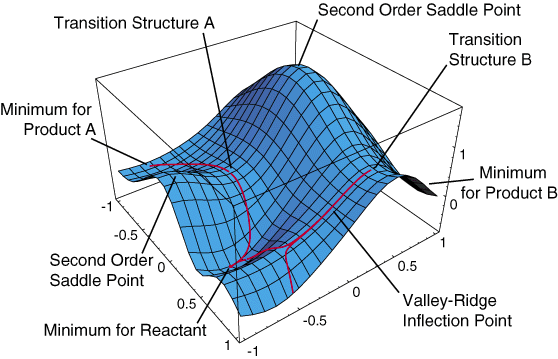
\includegraphics[scale=0.3]{PES}
\end{figure}

Questi punti di sella sono facilmente individuati da un'analisi della matrice hessiana, infatti in un'approssimazione armonica (quadratica) della PES, la matrice hessiana è la matrice delle costanti di forza armoniche e avrà quindi uno e un solo autovalore negativo che corrisponderà a una frequenza immaginaria. L'autovettore correlato a tale autovalore negativo rappresenta la direzione discendente verso un minimo.
I \emph{percorsi} che collegano i reagenti ai prodotti passando per gli \emph{stati di transizione} vengono definiti \emph{coordinate di reazione}. Queste coordinate sono delle \emph{continue} variazioni di geometria che permettono di passare da un minimo ad un altro con il minor impiego di energia possibile (cammino di minima energia o MEP). Se tali coordinate di reazione sono pesate per le masse prendono il nome di \emph{coordinate intrisiche di reazione} (IRC).
Dal momento che gli stati di transizione sono dei punti di sella, essi avranno, in una direzione preferenziale, concavità positiva. Lungo questa direzione è quindi possibile definire degli stati vibrazionali che saranno descritti da una forma potenziale approssimata a scelta. La bontà dell'approssimazione definisce l'accuratezza del modello scelto nel resituire i risultati corretti.
\section{Ottimizzazione di geometria}
Con \emph{ottimizzazione di geometria} si intende il processo di \emph{ricerca dei punti stazionari}, ovvero dei punti dove la risultante delle forze agenti sul sistema è nulla. Dato che è praticamente impossibile, anche per molecole di piccole dimensioni, ottenere una forma funzionale per tutta la superficie di energia potenziale, solitamente si ricercano direttamente i  punti stazionari con diverse tecniche. Tutte queste tecniche si basano sullo studio della PES mediante l'uso delle derivate; ciò è giustificato dal fatto che la forza agente su un sistema in meccanica classica viene descritta dall'Eq.\ref{grad}
\begin{equation}
\label{grad}
-\frac{\partial{V_x}}{\partial{x}}=F_x
\end{equation}
I diversi punti stazionari si differenziano in base ai valori che le derivate assumono in tali punti:
\begin{enumerate}
\item \textbf{Punti di minimo}
\begin{itemize}
\item Derivate prime (gradiente): Si devono annullare.
\item Derivate seconde (matrice hessiana): La matrice hessiana deve essere definita positiva.
\end{itemize}
\item \textbf{Punti di sella}
\begin{itemize}
\item Derivate prime (gradiente): Si devono annullare.
\item Derivate seconde (matrice hessiana): Almeno 1 autovalore della  matrice hessiana deve essere negativo.
\end{itemize}
\end{enumerate}
Il numero di autovalori negativi della matrice hessiana definisce l'\emph{indice} del punto stazionario e, gli autovettori associati a tali autovalori sono le direzioni lungo le quali la concavità negativa è massima. Tale vettore, detto \emph{vettore di transizione}, individua, di conseguenza, la direzione nella quale il sistema potrà evolvere dai reagenti ai prodotti con maggiore facilità, nel caso di un punto di sella. Punti critici che abbiano più di un autovalore negativo spesso corrispondono a punti di massimo, e sono, dunque, poco informativi.\\
In generale per ottenere le strutture associate ai punti stazionari si può procedere secondo 3 strategie:
\begin{enumerate}
\item Basate sull'energia; (metodo del simplesso, ricerca monovariata)
\item Basate sui gradienti; (gradienti coniugati, metodi quasi-Newton)
\item Basate sulle derivate seconde; (metodi Newton e Newton-Raphson) 
\end{enumerate}
I metodi \emph{basati sull'energia} sono quelli più generali, non dipendendo dalla natura della funzione che minimizzano, tuttavia vanno a convergenza molto lentamente. A causa di quest'ultima caratteristica non possono essere utilizzati in ogni tipologia di calcolo.
Agli antipodi rispetto a quest'ultimi troviamo i metodi \emph{basati sulle derivate seconde}, infatti questi sono in grado di individuare i punti di minimo andando a convergenza molto velocemente ma non tutte le forme funzionali sono adatte a questo tipo di algoritmo se le derivate seconde sono analitiche.
I metodi che riescono a bilanciare \emph{l'efficienza computazionale} e \emph{l'applicabilità} sono quelli \emph{basati sulle derivate prime}. Infatti essi risultano convenienti sia che le derivate prime siano analitiche, sia che esse siano numeriche. Inoltre, il campo di applicabilità riesce a coprire abbondantemente tutti i metodi tipicamente utilizzati in chimica computazionale.
\subsection{Metodi quasi-Newton}
In questa categoria di metodi la PES viene approssimata da una funzione quadratica rispetto al \emph{vettore spostamento delle posizioni atomiche} $\Delta x$ come mostrato in Eq.\ref{enquad}
\begin{equation}
\label{enquad}
E(x) = E_0 +g_0^t \Delta x + \frac{1}{2} \Delta x^t H \Delta x
\end{equation}
In Eq.\ref{enquad} $\Delta x=x-x_0$ ovvero la differenza tra la posizione attuale degli atomi e quella precedente, $H$ è la matrice hessiana e  $g$ è il gradiente valutato come in Eq.\ref{gradiente} al passo $t$.
\begin{equation}
\label{gradiente}
 g(x)=g_0+H \Delta x
\end{equation}
A partire dall'eq.\ref{gradiente} uguagliandola a $0$ si può ricavare un'espressione per $\Delta x$ come mostrato in Eq.\ref{newstep}
\begin{equation}
\label{newstep}
\Delta x= -H^{-1}g_0
\end{equation}
In seguito all'ottenimento della prima variazione delle posizioni atomiche ($\Delta x$)  per minimizzare l'energia si devono calcolare i tre parametri calcolati in Eq.\ref{enquad}  Eq.\ref{gradiente}  Eq.\ref{newstep}. A questo punto si confrontano i valori di hessiana gradiente e spostamento con dei valori limite (detti \emph{treshold}) scelti arbitrariamente in base alle necessità. Se i valori calcolati sono inferiori a quelli di \emph{treshold}, allora si sono verificate le \emph{condizioni di convergenza} e la minimizzazione si considera terminata. 
Un secondo metodo per terminare la minimizzazione è limitando il numero massimo di cicli in cui il programma ricalcola il passo di Newton. Così facendo si accorciano i tempi in cui si ottiene un risultato ma la \emph{convergenza non è garantita}.
In seguito a questi controlli si aggiorna la \emph{geometria} con quella generata dal passo di Newton. Si procede, dunque, ricalcolando $g$, $H$ e $\Delta x$ e nuovamente con i controlli. Questi passaggi vengono ripetuti ciclicamente fino al raggiungimento della convergenza come mostrato in figura \ref{algo}.

\begin{figure}[H]
\label{algo}
\centering
\caption{Diagramma di flusso relativo a un algoritmo di minimizzazione quasi Newton}
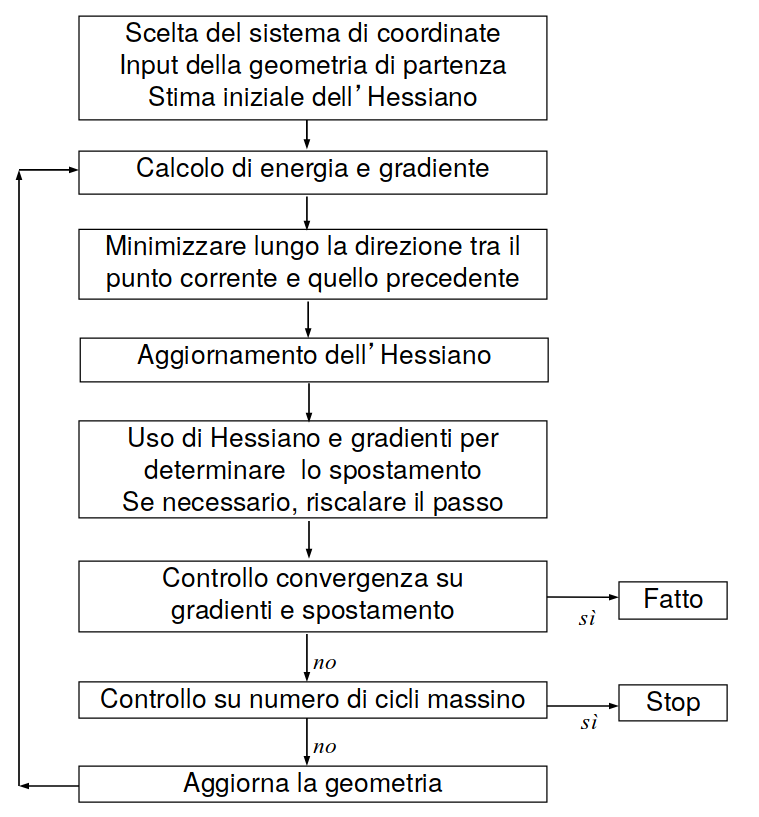
\includegraphics[scale=0.3]{quasiNewton}
\end{figure}
\subsection{Efficienza di metodi quasi Newton} 
L'efficienza di questi metodi dipende da 6 fattori principali:
\begin{enumerate}
\item \emph{Geometria iniziale}: Tanto più la geometria in input è vicina a lla condizione di minimo e tanto più velocemente sarà raggiunta la convergenza. Questi metodi ricercano il minimo più vicino, quindi non c'è nessuna garanzia che il minimo ottenuto sia un minimo globale. Semplicemente sarà il minimo locale più vicino alla geometria data in input.
\item \emph{Sistema di coordinate}: Oltre ai 2 metodi di definizione della geometria già citati, ovvero \emph{coordinate cartesiane} e \emph{coordinate interne}, si può verificare per alcuni tipi di molecole (tipicamente cicliche), che la definizione della geometria in termini di coordinate interne richieda un numero di parametri superiore a quello dei gradi di libertà. In questi casi le coordinate interne vengono definite \emph{ridondanti}. Al sistema di coordinate interne ridondanti ci si riferisce spesso come un metodo totalmente diverso per la definizione della geometria. Ciò avviene a causa delle migliori prestazioni, che le coordinate ridondanti garantiscono, nell'ottimizzazione di geometria. Infatti il numero di cicli di un algoritmo cala sensibilmente passando da un sistema cartesiano a uno di coordinate interne, e da uno di coordinate interne a uno di coordinate ridondanti.
\item \emph{Guess della matrice Hessiana}: Tanto più la matrice Hessiana sarà prossima a quella corretta e tanto più sarà rapida l'ottimizzazione. Il guess iniziale dipende, in prima analisi, dal sistema di coordinate: infatti un sistema cartesiano genererà matrici hessiane con pesanti \emph{termini extradiagonali} a causa dei forti accoppiamenti anarmonici; mentre in coordinate ridondanti la matrice assumerà una forma \emph{quasi diagonale}. A seconda della difficoltà del calcolo richiesto si possono scegliere diverse approssimazioni iniziali della matrice Hessiana:
\begin{itemize}
\item Matrice identità: calcoli semplici senza limiti nel numero di cicli;
\item Matrice ottenuta da calcoli semi empirici o di meccanica molecolare: calcoli semplici ma che possono richiedere molto tempo per andare a convergenza;
\item Matrice ottenuta da ottimizzazioni o calcoli di frequenze a un livello di teoria inferiore: calcoli complessi che non richiedono un elevato numero di cicli;
\item Matrice valutata numericamente o analiticamente (se possibile) allo stesso livello di teoria del calcolo richiesto: calcoli difficili con convergenza lenta.
\end{itemize}
\item \emph{Ricerca lineare}: Con ricerca lineare si intende il collegare con una linea monodimensionale ogni punto ottenuto sulla PES  a quello ottimizzato precedentemente e valutare la direzione del successivo secondo il criterio di massima pendenza. Così facendo si genera un'immagine della PES che non dipende da assunzioni di quadraticità o altro. Questa soluzione è infatti molto efficace, tuttavia non è molto efficiente in quanto può richiedere calcoli aggiuntivi per la valutazione della PES  nell'intorno di un punto calcolato. Si predilige quindi un approccio meno efficace, operando un \emph{best-fit polinomiale} della PES e ricercando il punto di minimo di tale polinomio. Ad ogni punto che si aggiunge alla PES si migliora la descrizione polinomiale dell'energia.
\item \emph{Metodo di aggiornamento della matrice Hessiana}: La matrice Hessiana non viene ricalcolata da zero a ogni ciclo (come nei metodi Newton) ma subisce un semplice aggiornamento ad ogni passo. I metodi che permettono di aggiornare la matrice Hessiana sono svariati: Murtagh-Sargent, Powell simmetrico, Davidson-Fletcher-Powell, Broyden-Fletcher-Goldfrab-Shanno (BFGS). Solo quest'ultimo viene usualmente utilizzato poiché permette di mantenere l'hessiana \emph{simmetrica} e \emph{definita positiva} minimizzando la \emph{norma della variazione della matrice hessiana}. Questi metodi sono utili solo con sistemi di piccole e medie dimensioni, per sistemi più complicati si rendono necessari metodi di tipo Newton o Newton-Raphson.
\item \emph{Controlli sulla lunghezza del passo di Newton}: Talvolta se si è lontani dal punto di minimo (gradiente elevato) o la PES è particolarmente piatta (autovalori dell'hessiana prossimi a 0), il passo di Newton calcolato con l'Eq.\ref{newstep} può superare il minimo e portare a strutture non ottimizzate. Si cerca quindi di limitare questi eventi impostando una lunghezza massima oltre la quale non è possibile estendere il passo di Newton. Questa lunghezza viene definita \emph{trust radius}, $\tau$.
\end{enumerate}
\section{Calcolo di frequenze vibrazionali}
I calcoli di frequenze vibrazionali sono la seconda grande categoria di calcoli che è possibile eseguire su un qualunque sistema chimico. Permettono, infatti, di predire una gran quantità di dati sperimentali. Tuttavia le tipologie di calcolo non si limitano a ottimizzazioni di geometria o a calcoli di frequenze ma includono una grande varietà di possibilità, ognuna delle quali permette di predire diverse proprietà chimico-fisiche del sistema analizzato. Il calcolo delle frequenze di vibrazione costituisce comunque un'ottima base per calcoli più complessi, in quanto, insieme all'ottimizzazione di geometria, fornisce come risultato la descrizione più completa della struttura nel punto di minimo. Infatti si aggiunge, con questo tipo di calcolo, all'informazione geometrica anche un'informazione sulle \emph{costanti di forza}.
Il calcolo fornisce, quindi informazioni aggiuntive rispetto all'ottimizzazione di geometria, dalla quale, quindi, non può prescindere.
\subsection{Passaggi del calcolo}
La  predizione delle frequenze di vibrazione si sviluppa attraverso i seguenti passaggi:
\begin{enumerate}
\item Esecuzione di un'\emph{ottimizzazione di geometria} al fine di collocare il sistema in un punto stazionario.
\item Calcolo della matrice delle \emph{derivate seconde} dell'energia rispetto alle coordinate cartesiane con l'origine nel centro di massa.
\item Costruzione della \emph{matrice delle costanti di forza pesata per le masse atomiche} ($W$), i cui elementi sono calcolati come in Eq.\ref{ForCon}.
\begin{equation}
\label{ForCon}
w_{ij} = \frac{1}{ \sqrt{m_i m_j} } \left( \frac{ \partial ^2E}{ \partial x_i \partial x_j} \right)= \frac{1}{\sqrt{m_i m_j}} H_{ij}
\end{equation}
In Eq.\ref{ForCon} $i$ e $j$ sono indici di coordinate atomiche quindi hanno come valore massimo $3N$, mentre $m_i$ e $m_j$ sono le masse degli atomi aventi coordinate $x_i$ e $x_j$. $H_{ij}$ è l'elemento $ij$ della matrice Hessiana.
\item Dato che si è operata un'ottimizzazione di geometria, e si ha la certezza di essere in un punto stazionario, si può procedere alla diagonalizzazione di $W$, come mostrato in Eq.\ref{diagw}. In questo modo si effettua un cambiamento di coordinate che da cartesiane passano a essere \emph{pesate per le masse}, mediante una trasformazione \emph{unitaria}. Questo nuovo sistema di coordinate è uno spazio vettoriale normato in cui le costanti di forza sono tra loro \emph{linearmente indipendenti}, quindi è come se potessimo visualizzare la singola vibrazione associata a ogni costante di forza isolata dalle altre. Abbiamo, quindi ricavato lo spazio dei \emph{modi normali di vibrazione} del sistema.
\begin{equation}
\label{diagw}
WL= L \Lambda
\end{equation} 
In Eq.\ref{diagw} $L$ è la matrice contenetnte gli autovettori di $W$ quindi la matrice dello \emph{spazio dei modi normali}, mentre $\Lambda$ è la matrice diagonale contenente le costanti di forza. La matrice $\Lambda$ conterrà 6 (o 5 per molecole lineari) autovalori nulli, corrispondenti ai gradi di libertà traslazionali e rotazionali, quindi i modi totali di vibrazione sono $3N-6$.
Le dimensioni di $\Lambda$ sono le stesse di $W$, ovvero $3N\times3N$ in quanto le costanti di forza sono calcolate tra ogni singola dimensione che definisce la posizione di un atomo e ogni altra dimensione che definisce la posizione di un altro atomo. Infatti atomi lontani avranno costanti di forza quasi nulle che aumenteranno al diminuire della distanza considerata. Da ciò possiamo dedurre che $W$ è sostanzialmente una matrice diagonale a blocchi e che $\Lambda$ sia invece semplicemente diagonale.
\item Calcolo delle frequenze vibrazionali a partire dagli autovalori di $W$ mediante l'Eq.\ref{freqvib}.
\begin{equation}
\label{freqvib}
\nu_k= \frac{\lambda_k^{1/2}}{2 \pi}
\end{equation}
\end{enumerate}
Le frequenze calcolate con Eq.\ref{freqvib} sono frequenze \emph{armoniche}; nel caso in cui il sistema includa atomi leggeri, queste possono essere sensibilmente diverse da quelle sperimentali perché gli effetti dell'anarmonicità diventano pesanti. Questi effetti possono essere considerati mediante l'uso di metodi perturbativi. 
Un esempio di applicazione delle frequenze vibrazionali è il calcolo dell'\emph{energia di punto zero} (ZPE). Essa è un parametro efficaciemente utilizzato per fare semplici confronti tra energie di diversi sistemi. Viene calcolata dall'Eq.\ref{ZPE}.
\begin{equation}
\label{ZPE}
E_{ZPE}=\frac{1}{2} \sum \limits_{k=1}^{3N-6}h\nu_k
\end{equation}
Questa energia descrive l'energia più bassa assumibile da un qualsiasi sistema quantistico. Il suo utilizzo principale sta nella previsione di differenze di energia tra sistemi quantistici, infatti tutti paramaetri termodinamici macroscopici possono essere determinati a partire da considerazioni microscopiche mediante l'uso della termodinamica statistica, la quale coinvolge valori di differenze di energia ricavabili come riportato in Eq.\ref{ZPE}. Il limite principale dell'uso della ZPE sta nel fatto che si assume che la molecola si trovi a $0 K$ quindi ogni effetto dinamico o dipendente dalla temperatura non può essere osservato. Per poter fare previsioni a temperature superiori sono necessari calcoli più complessi e quindi più costosi in termini temporali.


\part{Meccanica molecolare}
\chapter{Metodi basati su campi di forza}
Il principale obbiettivo di un metodo di calcolo è giungere a un'espressione numerica dell'energia totale del sistema analizzato. Il punto fondamentale in ogni metodo, quantistico o classico, è la definizione dell'\emph{energia elettronica} \index{energia !elettronica}che nell'approssimazione di Born-Oppenheimer coincide con l'energia totale della molecola a meno del potenziale di interazione tra nuclei. Infatti nei metodi quantistici questa è definita a partire dalla risoluzione dell'equazione di Schr\"{o}dinger, mentre nei metodi della meccanica molecolare, l'energia elettronica è definita come una \emph{funzione parametrica} delle coordinate nucleari. I parametri che compaiono nella funzione sono tipicamente determinati in base a  dati sperimentali o computazionali calcolati a un più alto livello di teoria.
Ogni effetto quantistico, quando si utilizzano metodi di meccanica molecolare, viene \emph{trascurato}. Quindi per sistemi dipendenti dal tempo la dinamica verrà trattata esclusivamente in base alla 2° legge della dinamica di Newton, mentre per sistemi indipendenti dal tempo il problema sta semplicemente nel calcolare l'energia totale della geometria in input.

\section{I tipi atomici}
\begin{figure} 
\label{atomty}
\centering
\caption{Esempio di un gruppo funzionale con i diversi tipi atomici  messi in evidenza}
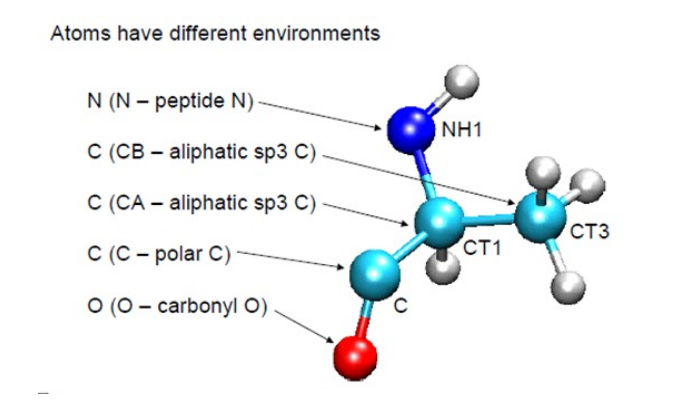
\includegraphics[scale=0.3]{tipiAtomici}
\end{figure}
Negli anni '30 si notò dall'osservazione degli spettri vibrazionali delle molecole che assemblamenti uguali di atomi condividevano le stesse proprietà chimico-fisiche. Da queste osservazioni nacque il concetto di \emph{gruppo funzionale} \index{gruppo funzionale}. In ambito computazionale si può pensare, quindi, di definire la geometria molecolare di input in base a degli atomi parametrizzati in modo da poter appartenere a uno specifico gruppo funzionale. Questo è necessario in quanto una trattazione classica non permette di determinare la corretta struttura elettronica che definisce un atomo in un gruppo funzionale. Nei metodi della meccanica quantistica questo problema è assente e si può quindi far uso di atomi puri privi di ulteriori parametrizzazioni se non quelle relative alla struttura interna del nucleo.
Questi atomi parametrizzati che entrano a far parte dei vari gruppi funzionali prendono il nome di \emph{tipi atomici} \index{tipi atomici}. Essi sono definiti dai parametri nucleari e dal tipo di legame che coinvolge l'atomo, quindi dal gruppo funzionale in cui si trova come si può osservare in Fig.\ref{atomty}.1.

Tipicamente i \emph{tipi atomici} prendono il nome in base all'ordine in cui sono stati parametrizzati secondo un codice alfabetico o numerico come riportato nella Fig.\ref{mm2at}.2.

\begin{figure} [H]
\label{mm2at}
\centering
\caption{Codice numerico utilizzato per la nomenclatura dei tipi atomici  nel campo di forza MM2}
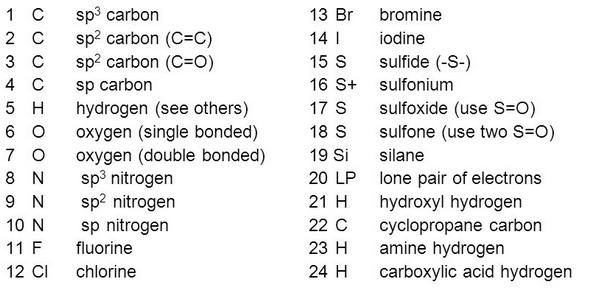
\includegraphics[scale=0.3]{mm2at}
\end{figure}
Altri campi di forza possono utilizzare diverse definizioni di tipi \index{tipi atomici} atomici a seconda dello scopo che si prefiggono. Infatti campi di forza messi a punto per calcolare le proprietà di molecole biologiche di grandi dimensioni come GROMOS o AMBER, faranno uso di tipi atomici che, invece di definire il singolo atomo, definiranno un assemblamento di atomi, come un amminoacido o un nucleotide. In questo modo i calcoli per questo tipo di molecole risulteranno molto più veloci se eseguiti con il campo di forza adeguato.
\section{Campo di forza}
Il \emph{campo di forza} \index{campo di forza} è il concetto alla base di ogni metodo di meccanica molecolare\index{meccanica molecolare}. Esso è, infatti, quella \emph{funzione parametrica delle coordinate nucleari} che definisce la superficie di energia potenziale rappresentabile come $E=E(\mathbf{k},\mathbf{q})$, dove $\mathbf{k}$ è il vettore contenente i parametri e $\mathbf{q}$ è il vettore delle coordinate nucleari.
In generale è conveniente scrivere un campo di forza come somma di singoli contributi aventi senso fisico. Quindi possiamo esprimere l'energia come in Eq.\ref{ForF}.
\begin{equation}
\label{ForF}
E= E_{str}+E_{bend}+E_{tors}+E_{VdW}+E_{el}+E_{cross}
\end{equation}
Con:
\begin{itemize}
\item $ E_{str}$: Contributo all'energia dovuto allo \emph{stretching} dei legami;
\item $E_{bend}$: Contributo all'energia dovuto al \emph{bending} dei legami;
\item $E_{tors}$: Contributo all'energia dovuto alla \emph{torsione} dei legami;
\item $E_{VdW} $: Contributo all'energia dovuto all'\emph{ingombro sterico} degli atomi;
\item $E_{el}  $: Contributo all'energia dovuto all'\emph{elettrostatica} delle cariche;
\item $E_{cross}$: Contributi misti all'energia dovuti all'accoppiamento dei moti di \emph{stretching-bending}, \emph{stretching-torsione} e \emph{bending-torsione}\\ ($E_{cross}=E_{str/bend}+E_{str/tors}+E_{bend/tors}$).
\end{itemize}
La procedura di \emph{ottimizzazione \index{ottimizzazione}} prevede, quindi, la minimizzazzione del campo di forza rispetto alle coordinate nucleari mediante i metodi analizzati nel capitolo $1$ per la ricerca dei minimi, ovvero l'annullamento delle derivate prime come in Eq.\ref{optff} a partire da una geometria iniziale $Q_N^0$.
\begin{equation}
\label{optff}
E_{FF}^0(Q_N^0)\longrightarrow \frac{\partial E_{FF}^0}{\partial Q_N}=0 \longrightarrow E_{FF}(Q_N)
\end{equation}
Di seguito i singoli contributi al campo di forza verranno analizzati, mettendo in evidenza le diverse forme funzionali proposte e i problemi a esse correlati.
\subsection{L'energia di stretching \index{energia !di stretching}} L'energia di stretching è l'energia associata all'allungamento del legame \emph{tra due tipi atomici}, quindi in una molecola biatomica. Nella sua forma funzionale più semplice può essere vista come un'espansione in \emph{serie di Taylor \index{serie !di Taylor}} intorno a un punto di equilibrio, corrispondente alla lunghezza media del legame ($R_0$). 
\begin{equation}
\label{tayxp}
 E_{str}(R^{AB}-R^{AB}_0)= E(0)+   \frac{d E}{d R} \biggr \rvert_{R_0} (R^{AB}-R_0^{AB})+\frac{1}{2}\frac{d^2E}{dR^2} \biggr \rvert_{R_0} (R^{AB}-R_0^{AB})^2
\end{equation} 
Nell'Eq.\ref{tayxp} lo sviluppo viene troncato al secondo ordine, ovvero al primo termine non nullo, infatti $E(0)$ è tipicamente posto $=0$, in quanto costituisce il punto zero dell'energia. Mentre il termine $\frac{d E}{d R}  (R^{AB}-R_0^{AB})$ si considera $=0$ nei pressi del punto di minimo, in quanto il potenziale in tale zona ha un comportamento praticamente armonico e la derivata di una funzione quadratica nei pressi del minimo tende a $0$ molto più velocemente della funzione stessa.
Dal momento che le derivate sono valutate in $R_0$ tali termini sono costanti e l'equazione \ref{tayxp} si semplifica notevolmente come illustrato in Eq.\ref{str2}.
\begin{equation}
\label{str2}
E_{str}(R^{AB}-R^{AB}_0)=k^{AB}(R^{AB}-R_0^{AB})^2=k^{AB}(\Delta R^{AB})^2
\end{equation}
In Eq.\ref{str2} la costante $k^{AB}$ è la costante di forza del legame, che viene visto come un oscillatore armonico \index{oscillatore armonico}. Questa approssimazione armonica è la più semplice che si possa costruire e funziona bene con sistemi di piccole dimensioni in cui i legami non siano sottoposti a tensioni particolarmente elevate. In tali casi i valori calcolati con questa approssimazione si scostano significativamente dai valori sperimentali ottenuti dagli spettri vibrazionali.
Al fine di migliorare il campo di forza e permettere la descrizione anche di sistemi più complessi è necessario complicare la forma funzionale riportata in Eq.\ref{str2} superando l'approssimazione armonica.
Il modo più semplice per fare ciò consiste nell'aggiungere ulteriori termini, precedentemente trascurati, all'espansione di Taylor. Questo approccio è molto semplice ma presenta $2$ grandi svantaggi:
\begin{itemize}
\item Il numero di parametri da definire aumenta e con esso la distanza da un approccio \emph{ab initio};
\item Il comportamento al limite $R\rightarrow\infty$ (dissociazione della molecola) delle funzioni polimoniali è totalmente diverso dal caso reale.
\end{itemize}
Il problema principale è dovuto al comportamento al limite dissociativo, infatti la funzione reale per una distanza infinita tende all'energia di dissociazione della molecola. Ciò non avviene per le funzioni polinomiali, ma è possibile individuare delle semplici funzioni che soddisfano questo criterio, come la funzione di Morse o potenziale di Morse \index{potenziale !di Morse} riportata in Eq.\ref{morse}.
\begin{equation}
\label{morse}
E_{Morse}(\Delta R)= D(1-e^{\sqrt{k/2D}\Delta R})^2
\end{equation}
Nell'equazione di Morse (Eq.\ref{morse}) $D$ è l'energia di dissociazione e $k$ è la costante di forza dell'oscillatore rigido. Nonostante il comportamento quasi corretto del potenziale di Morse per separazioni tendenti all'infinito, quando ci si trova nei pressi del minimo (fino a $40$ $kJ/mol $ dal minimo) il comportamento non è siginificativamente diverso da quello di un potenziale armonico. La differenza sostanziale risiede dunque nel numero di parametri necessari a definire i diversi potenziali, infatti il potenziale di Morse fa uso di $2$ parametri contro la sola costante di forza usata in un potenziale armonico. Da queste ultime cosiderazioni si può accantonare l'ipotesi di utilizzare il potenziale di Morse e cercare un modo di diminuire il numero di parametri necessari a una approssimazione polinomiale troncata a un ordine superiore al secondo. 
Per ridurre il numero di parametri in una approssimazione di Taylor esistono diversi modi ma i $3$ principali sono:
\begin{itemize}
\item Considerare le costanti di forza degli ordini superiori come frazioni di quella al secondo ordine (qualsiasi fosse il numero di parametri viene ridotto a $1$);
\item Far coincidedere la derivata $n-$esima dell'espansione di Taylor con la derivata $n-$esima del potenziale di Morse. In questo modo i parametri vengono ridotti a $2$ ovvero $k$ e $D$;
\item Permettere alla costante di forza di variare con la distanza di legame.
\end{itemize}
In figura \ref{morsepot} è possibile vedere le differenze tra le diverse approssimazioni e il potenziale esatto.

\begin{figure} 
\label{morsepot}
\centering
\caption{Confronto tra le diverse approssimazioni di $E_{str}$. Con "\emph{Exact}" si intende calcolato a un livello superiore di teoria ([$8,8$]-CASMP$2$/aug-cc-pVTZ). P$2$ e P$4$ sono le approssimazioni polinomiali troncate al secondo e al quarto ordine.}
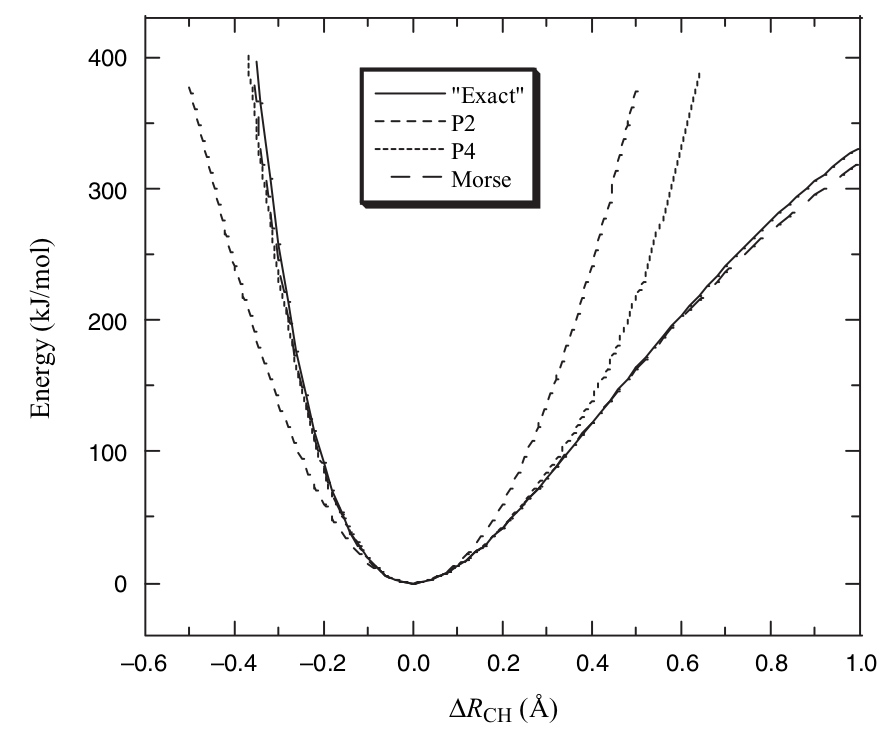
\includegraphics[scale=0.4]{morsepot}
\end{figure}

\subsection{L'energia di bending \index{energia !di bending}}
L'\emph{energia di bending} è l'energia necessaria a variare un angolo tra  $3$ atomi. In analogia con $E_{str}$ si può sviluppare in serie anche $E_{bend}$ nell'intorno del valore di equilibrio dell'angolo naturale del sistema in esame. Tale sviluppo in serie può essere, quindi, troncato al secondo ordine in perfetta analogia con l'energia di stretching come mostrato in equazione \ref{entors}.
\begin{equation}
\label{entors}
E_{bend}(\theta^{ABC}-\theta^{ABC}_0)= k^{ABC} (\theta^{ABC}-\theta^{ABC}_0)^2
\end{equation}

Anche in questo caso potrebbe essere necessario un miglioramento nella descrizione della forma funzionale, infatti si può espandere a ordini superiori la serie di Taylor procedendo con le stesse approssimazioni delle costanti adottate per l'energia di stretching. In questo caso, nonostante i miglioramenti apportati alla forma funzionale i risultati presentano deviazioni minime dall'approssimazione armonica. Tali miglioramenti, tuttavia, non si giustificano a causa dell'aumento di parametrizzazione e quindi di complessità del calcolo.
La maggior parte dei sistemi chimici è adeguatamente descritta da un'approssimazione armonica, tuttavia esistono alcune specie soggette a geometrie particolari come atomi di C $sp^2$ piramidalizzati che deviano totalmente da un comportamento armonico. Per risolvere tali situazioni di \emph{bending fuori dal piano} (out of plane oop) si può aggiungere un termine all'energia di bending da applicare esclusivamente con determinati tipi atomici. Quindi riscriviamo l'energia di bending come $ E_{bend}=E_{ip}+E_{oop}$ dove $E_{oop}$ viene definito come il termine del secondo ordine di un'espansione di Taylor in termini della distanza dal piano come si può osservare dalla Fig.\ref{oopf} e dal Eq.\ref{oope}.

\begin{equation}
\label{oope}
E_{oop}(d)= k^Bd^2
\end{equation}

\begin{figure} 
\label{oopf}
\centering
\caption{Tipico sistema piramidale soggetto a bending fuori dal piano}
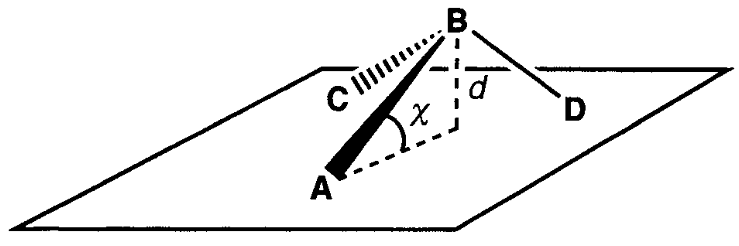
\includegraphics[scale=0.4]{oop}
\end{figure}
L'espansione in serie di Taylor può essere anche fatta in termini dell'angolo $\chi$ formato tra i legami e il piano su cui giacciono i tre atomi A D C. 


\subsection{L'energia torsionale \index{energia !torsionale}}
L'energia torsionale è l'energia associata a un cambiamento conformazionale  in una molecola che abbia almeno 4 atomi e che possa essere visualizzata in proiezione di Newman \index{proiezione !di Newman}.
Essa si distingue dalle energie di stretching e bending in $3$ aspetti:
\begin{enumerate}
\item L'energia torsionale e i suoi parametri \emph{non dipendondo da interazioni di legame };
\item L'energia torsionale deve avere un comportamento \emph{periodico} con la variazione dell'angolo;
\item Non è possibile usare un'espansione di Taylor perché a causa dei valori bassi dell'energia torsionale è praticamente impossibile stabilire un valore di equilibrio.
\end{enumerate}

Dato che si rende necessario soddisfare il vincolo della periodicità, la scelta più facile sta nell'optare per un'espansione in serie di Fourier \index{serie !di Fourier} come riportato in Eq.\ref{fou}.
\begin{equation}
\label{fou}
E_{tors}(\omega)=\sum \limits _{n=1} V_n \cos (n\omega)
\end{equation}

In Eq.\ref{fou} $V_n$ è il valore di barriera energetica per la rotazione intorno al legame, e talvolta può anche essere nullo a seconda degli atomi coinvolti. Nelle molecole più semplici a elevata simmetria solitamente solo i termini pari o dispari hanno valori non nulli.
In sistemi con più di $4$ atomi, come nell'etano sostituito, le conformazioni assumibili diventano più numerose e con energie diverse come mostrato in Fig.\ref{conf}. Per descrivere questo comportamento diventa necessario considerare altri termini. Solitamente l'aggiunta del termine $n=1$ risolve questi problemi.
Nella maggior parte dei casi non è necessario andare oltre al termine $n=3$ per avere una descrizione corretta del sistema.

\begin{figure} [H]
\label{conf}
\centering
\caption{Andamento dell'energia conformazionale per una serie di Fourier con parametri: $V_1=0.5$, $V_2=-0.2$, $V_3=0.5$}
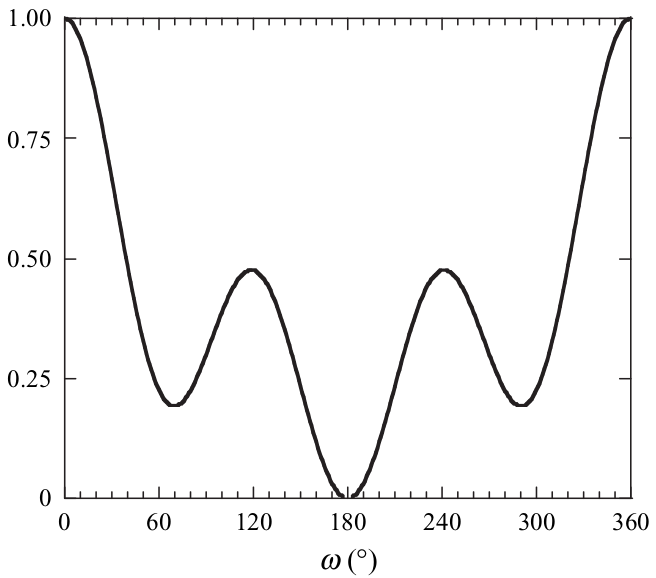
\includegraphics[scale=0.4]{conf}
\end{figure}

Un'interessante applicazione dell'energia torsionale deriva dalla sua applicazione nella descrizione dei \emph{bending fuori dal piano}\index{bending fuori dal piano}. Infatti applicando l'energia torsionale anche a questi casi, è possibile evitare l'inserimento di un termine apposta. Per fare ciò bisogna considerare $\omega$ come riportato in Fig.\ref{omconf}.

\begin{figure} [H]
\label{omconf}
\centering
\caption{Definizione di $\omega$.}
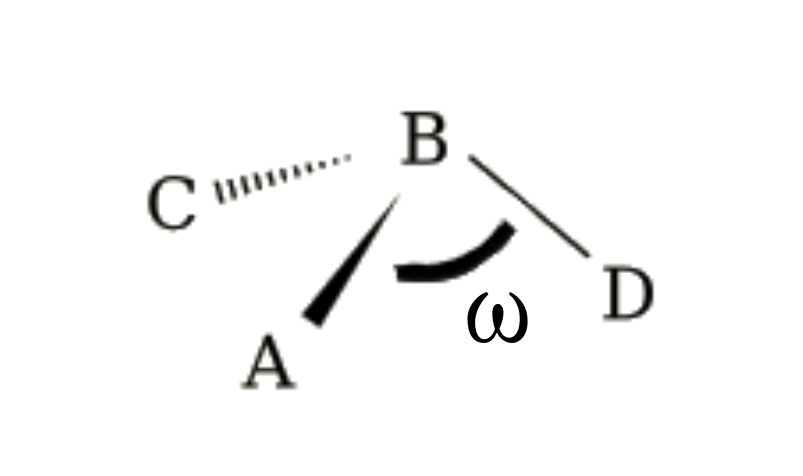
\includegraphics[scale=0.2]{omconf}
\end{figure}

\subsection{L'energia di Van der Waals\index{energia !di Van der Waals}}
L'energia di \emph{Van der Waals} è, unitamente ai contributi coulombiani, una delle due forme di energia di \emph{non legame}. Infatti questa forma di interazione intercorre tra atomi che non essendo legati si ritrovano vicini a causa di moti molecolari o altri impedimenti di natura geometrica. Possiamo visualizzare quest'energia come quella parte \emph{non polare} delle interazioni non dovute a cariche elettriche. Esse sono tipicamente molto deboli, infatti a grandi distanze sono nulle, tuttavia se 2 atomi sono sufficientemente vicini questa forma di interazione diventa importante per la reattività chimica.\\
\subsubsection{L'origine del fenomeno} 
Questa attrazione che si verifica esclusivamente su brevi distanze, può essere ricondotta a un particolare tipo di interazione dipolare. Infatti i dipoli che consideriamo sono \emph{dipoli istantanei\index{dipoli istantanei}}, dovuti alle infinite fluttuazioni statistiche della densità elettronica intorno agli atomi. 
Quando due atomi si avvicinano il dipolo istantaneo di uno induce un dipolo istantaneo nell'altro. Ciò genera un'interazione attrattiva tra i due atomi. Le interazioni attrattive non sono esclusivamente di tipo \emph{dipolo-dipolo} ma possono contribuire anche multipoli istantanei, tuttavia questi hanno un peso nettamente inferiore rispetto all'interazione dipolo-dipolo.
Una volta che l'interazione attrattiva termina i due atomi continuano ad avvicinarsi finché le due densità elettroniche non entrano in contatto tra loro. Ciò genera un interazione repulsiva molto più forte in quanto dovuta all'elettrostatica.
Teoricamente è stato predetto che questa interazione decade come ${1}/{r^6}$.  \\
\subsubsection{La forma funzionale} In base alle considerazioni qualitative sul comportamento che due atomi interagenti secondo l'energia di Van der Waals possiedono, possiamo dedurre una prima approssimazione della funzione che descriverà questa interazione. Descriviamo quindi questa funzione come somma di un contributo attrattivo (segno negativo) e uno repulsivo (segno positivo) in Eq.\ref{som}

\begin{equation}
\label{som}
E_{VdW}(R^{AB})=E_{repulsione}(R^{AB})-\frac{C^{AB}}{(R^{AB})^6}
\end{equation}

In Eq.\ref{som} risulta evidente la dipendenza dall'\emph{inverso della sesta potenza} come teoricamente predetto, tuttavia dato che la parte repulsiva non può essere predetta da calcoli teorici, la sua forma funzionale non è implicita.
Per ovviare a questo problema nel corso del tempo sono state proposte diverse funzioni atte a descrivere l'interazione repulsiva. Tutte queste proposte mantengono sostanzialmente invariata la dipendenza dall'inverso del raggio ma si distinguono esclusivamente per l'ordine della potenza, vengono quindi spesso chiamate secondo il codice $[x,y]$ dove $x$ e $y$ sono rispettivamente la potenza del \emph{termine repulsivo} e quella del \emph{termine attrattivo} Di seguito vengono analizzate le principali funzioni proposte e confrontate tra loro e rispetto ai dati sperimentali.\\


\subsubsection{Il potenziale di Lennard-Jones\index{potenziale !di Lennard-Jones}}
Quello di \emph{Lennard-Jones} è un potenziale $[12,6]$ descritto dall'equazione \ref{lj}.
\begin{equation}
\label{lj}
E_{LJ}(R)=\epsilon \biggr[ \biggr( \frac{R_0}{R} \biggr)^{12} -2 \biggr( \frac{R_0}{R}  \biggr)^{6}  \biggr]
\end{equation}
In Eq.\ref{lj} $R_0$ è  la distanza alla quale il sistema ha il punto di minimo mentre $\epsilon$ è la profondità del punto di minimo.
Alternativamente può essere scritta in termini della \emph{sezione d'urto} ($\sigma = 2^{-(1/6)}R_0 $) ottenendo l'equazione \ref{lj2}.
\begin{equation}
\label{lj2}
E_{LJ}(R)=4 \epsilon \biggr[ \biggr( \frac{\sigma}{R} \biggr)^{12} - \biggr( \frac{\sigma}{R}  \biggr)^{6}  \biggr]
\end{equation}
La scelta di utilizzare un esponente $12$ per la parte repulsiva è dettata esclusivamente dal fatto che tale esponente mostra un'\emph{efficienza computazionale} superiore a esponenti che magari garantiscono accuratezza migliori come $9$ e $10$.\\

\subsubsection{Il potenziale di Buckingham o Hill\index{potenziale !di Buckingham o Hill}}
Dato che, come è noto, la densità elettronica \emph{decade esponenzialmente con la distanza} dal nucleo, ricordando la parte radiale dell'atomo di idrogeno, è giustificata teoricamente la scelta di una funzione esponenziale per la parte repulsiva. Potenziali che fanno uso di una simile funzione vengono chiamati "di Buckingham" o "di Hill", e la loro forma funzionale generale è riportata in Eq. \ref{bh}.
\begin{equation}
\label{bh}
E_{BH}(R)=A e^{-BR}-\frac{C}{R^6}
\end{equation}
Dove $A$, $ B$ e $ C$ sono costanti arbitrarie dipendenti da $R_0$, $\epsilon$ e da 
un parametro $\alpha$ da ottimizzare.
Questo potenziale ha un accordo con i dati sperimentali migliori rispetto a Lennard-Jones ma per distanze molto piccole ($R\rightarrow0$) l'esponenziale assume valori costanti mentre il termine attrattivo tende a $-\infty$ risultando quindi in una \emph{fusione nucleare}. Ovviamente un tale risultato è privo di senso e i potenziali di questo tipo diventano totalmente inapplicabili a distanze troppo ridotte.\\

\subsubsection{Il potenziale di Morse\index{potenziale !di Morse}}
Anche il potenziale di Morse può essere utile per rappresentare la somma di questi due contributi. Ma necessita un paio di modifiche nei valori numerici dei parametri che include.
La forma funzionale rimane invariata rispetto quella mostrata in Eq.\ref{morse} ma viene comunque riportata.

\begin{equation}
\label{morse2}
E_{Morse}(\Delta R)= D(1-e^{\sqrt{k/2D}\Delta R})^2
\end{equation}

L'assenza del termine attrattivo in $R^{-6}$ non è un problema in quanto in realtà considerando esclusivamente quel termine si trascurano dei termini aggiuntivi con potenze superiori che produrrebbero una curva analoga a quella di Morse.\\
Tra tutti questi potenziali quelli che  garantiscono i risultati più accurati sono \emph{Buckingham} e \emph{Morse} come si vede in Fig.\ref{vdwfig}, tuttavia il più usato è \emph{Lennard-Jones} poiché non necessita del calcolo di $R_0$, che in coordinate cartesiane risulta particolarmente dispendioso, invece avvalendosi della sezione d'urto, facilmente calcolabile, permette di risparmiare ingenti quantità di tempo.

\begin{figure} [H]
\label{vdwfig}
\centering
\caption{Confronto tra i vari potenziali.}
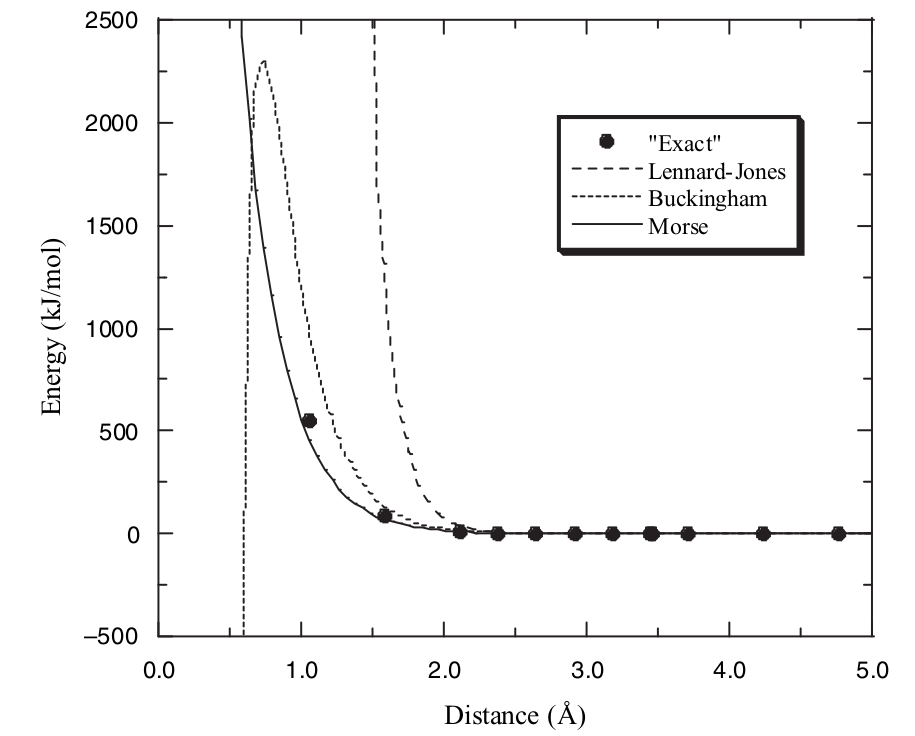
\includegraphics[scale=0.3]{vdw}
\end{figure}

\subsubsection{Parametrizzazione dei potenziali}
In ogni caso analizzato fin'ora il potenziale è sempre dipeso da $2$ parametri:
\begin{itemize}
\item $R_0$ ovvero la distanza a cui si manifesta il punto di minimo;
\item $\epsilon$ ovvero la \emph{morbidezza} (softness) dell'atomo.
\end{itemize}
Per quanto riguarda la morbidezza dell'atomo, si intende la \emph{propensione} della densità elettronica a \emph{polarizzarsi spazialmente}. Maggiore è la morbidezza e maggiore è la probabilità che la densità elettronica non sia sferica, assunzione sulla quale si fondano i metodi di ottimizzazione di geometria. Per ovviare a questo problema esistono $2$ metodi:
\begin{enumerate}
\item Spostare la posizione del nucleo anisotropo lungo la direzione di legame. Ciò permette di introdurre l'anisotropia ma non l'inserimento di \emph{lone-pair};
\item Introduzione di \emph{pseudo-atomi\index{pseudo-atomi}} ovvero degli atomi privi di massa e carica e più piccoli dell'idrogeno circondati da una precisa densità eletrronica a seconda del tipo atomico che descrivono. Tali \emph{pseudo-atomi} vengono quindi posti nello spazio dei \emph{lone-pair} o delle polarizzazioni modificando la densità elettronica circostante. 
\end{enumerate}
\subsubsection{Il legame a idrogeno \index{legame !a idrogeno} \label{mimmo}}
Viene tipicamente modellizzato da un potenziale di Lennard-Jones $[12,10]$. Tuttavia non riuscendo a descrivere, in una simile trattazione, la dipendenza dall'orientazione si può includere un  termine \textit{ad hoc} che dipende dall'angolo X-H-Y.



\subsection{L'energia elettrostatica: Cariche atomiche\index{energia !elettrostatica}}
Questa forma di energia costituisce la seconda parte delle interazioni non leganti, insieme alle interazioni di Van der Waals \index{energia !di Van der Waals}.
Queste interazioni sono dovute alla presenza di dipoli fissi generati dalla differenza di carica tra gli atomi legati come nel caso del gruppo carbonilico.
Per poter modellizzare questo tipo di interazione esistono sostanzialmente $2$ approcci semplici:
\begin{itemize}
\item Dotare i singoli atomi di cariche parziali \index{cariche parziali};
\item Collocare un \emph{momento dipolare} \index{momento !dipolare}su ogni legame.
\end{itemize}
Entrambi questi metodi danno risultati praticamente identici a distanze elevate mentre sul corto raggio la distinzione tra le diverse cariche della molecola diventa importante e non è quindi più possibile avere risultati identici.
\subsubsection{Il metodo delle cariche parziali}
\begin{equation}
\label{culo}
E_{el}(R^{AB})= \frac{Q^AQ^B}{\epsilon R^{AB}}
\end{equation}
L'energia di interazione viene descritta in modo \emph{coulombiano} (Eq.\ref{culo}), le cariche parziali assegnate agli atomi $A$ e $B$ sono determinate da regole empiriche o mediante regressione lineare a partire da dati calcolati con metodi della meccanica quantistica o mediante fitting alla funzione di Potenziale elettrostatico o ESP (Eq.\ref{esp}). Tale fitting viene svolto numericamente campionando la ESP in una gliglia di punti.

\begin{equation}
\label{esp}
\Phi_{esp}(r)= \sum \limits_{A}^{N_{nuc}} \frac{Z_A}{\vert R_A-r \vert}-\int \frac{\rho (r')}{\vert r'-r \vert}dr'
\end{equation}

\subsubsection{Il metodo dei dipoli}
\begin{equation}
\label{dipollo}
E_{el}(R^{AB})= \frac{\mu ^A \mu ^B}{\epsilon( R^{AB}     )^3} (\cos \chi - 3 \cos \alpha_A \cos \alpha _B   )
\end{equation}
In Eq.\ref{dipollo} gli angoli sono definiti come in Fig.\ref{diocancro}.

\begin{figure} [H]
\label{diocancro}
\centering
\caption{Definizioni degli angoli per l'interazione dipolare}
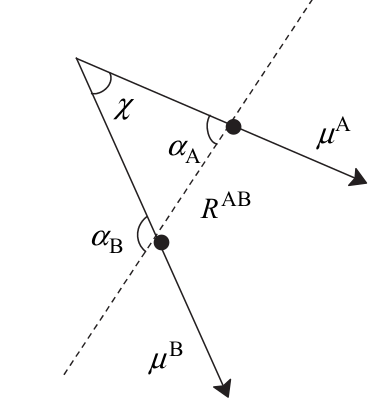
\includegraphics[scale=0.3]{dipoli}
\end{figure}
Data la difficoltà nella parametrizzazione dei metodi basati sui dipoli, tendenzialmente si preferisce far uso del metodo delle cariche parziali.

Il parametro più importante da determinare è $\epsilon$, poiché, in quanto \emph{costante dielettrica} permette di modellizzare la presenza di \emph{solventi}. Alcuni campi di forza permettono alla costante dielettrica di variare con la distanza e, sebbene non ci sia una valida giustificazione teorica, ottengono così facendo dei risultati in buono accordo coi dati sperimentali.
Dato che, come per l'energia di Van der Waals\index{energia !di Van der Waals},  il costo del calcolo aumenta velocemente all'aumentare delle coppie di atomi considerate, si rende necessario porre un limite alla distanza entro la quale calcolare questi contributi. La maggior parte dei campi di forza trascura le interazioni elettrostatiche per distanze inferiori ai $2$ legami inziando quindi a considerare solo le interazioni a $4$ atomi.
Altri campi di forza, calcolano le interazioni di non legame a partire dal \emph{terzo} atomo, mescolando però i contributi di bending e stretching. Tali campi di forza vengono chiamati di Urey-Bradley.

I tipi atomici\index{tipi atomici}, per loro natura, vengono parametrizzati in modo rigido, e quindi sono inevitabilmente inadatti a descrivere ogni possibile situazione. In particolare, nell'ambito delle interazioni elettrostatiche, capita spesso che le cariche parziali assegnate possano variare in seguito a modifiche geometriche come semplici cambiamenti conformazionali. Ciò comporta $3$ problemi:
\begin{enumerate}
\item Le cariche che dipendono da cambiamenti conformazionali possono essere modellizzate a partire da \emph{cariche fluttuanti\index{cariche fluttuanti}} o \emph{modelli di polarizzazione\index{modelli di polarizzazione}};
\item La scelta della griglia di campionamento del ESP (Eq.\ref{esp}) e il numero di atomi inclusi nel fitting determinano le cariche dei tipi atomici. Dato che solo gli atomi 	\emph{superficiali} avranno un'influenza importante sulla forma della ESP, essi saranno gli unici di cui si otterrà un valore di carica, tuttavia tale valore sarà poco accurato a causa della presenza degli atomi interni. Tendenzialmente si aggiungono quindi dei termini che escludono i tipi atomici più interni per calcolare accuratamente almeno quelli superficiali;
\item L'accuratezza assoluta di questi metodi tuttavia non è garantita a causa del fatto che, considerando esclusivamente cariche puntuali, vengono totalmente trascurati gi effetti dei multipoli che vengono quindi aggiunti artificialmente senza che abbiano un atomo di riferimento. 
\end{enumerate}
\subsection{L'energia elettrostatica: Multipoli atomici\index{energia !elettrostatica}}\label{ee2}

Uno degli obbiettivi più difficili da raggiungere nella creazione di un campo di forza è un'accurata descrizione delle interazioni elettrostatiche \emph{intermolecolari}. Ciò non avviene se si fa uso di cariche atomiche fisse per $ 5$ motivi:
\begin{enumerate}
\item Il fit delle cariche atomiche è incentrato sul descrivere interazioni \emph{intramolecolari};
\item L'uso di cariche parziali produce errori anche di $10-20$ $kJ/mol$;
\item Gli effetti di penetrazione di carica tra le nuvole elettroniche sono trascurati;
\item Gli accoppiamenti delle cariche atomiche ed eventuali momenti di ordine superiori con la geometria non vengono considerati;
\item Si considerano solo interazioni a $2$ corpi quando, talvolta, il peso dell'interazione a $3$ corpi può pesare fino al $20\%$
\end{enumerate}

I termini energetici di non legame contribuiscono insieme all'\emph{energia torsionale}\index{energia !torsionale} alla determinazione dei \emph{gradi di libertà conformazionali}. Infatti nei \emph{sistemi non polari} è possibile descrivere questi gradi di libertà esclusivamente mediante $E_{VdW}$ e $E_{tors}$. Mentre se si analizzano sistemi polari l'energia associata a un cambiamento conformazionale è \emph{dominata da } $E_{el}$. Tuttavia essa è in dipendenza diretta con l'energia torsionale. Risulta quindi chiaro che se l'energia torsionale non è descritta accuratamente per ogni dimensione del sistema (ovvero ha poca trasferibilità) allora non sarà possibile avere una descrizione accurata nemmeno per l'energia elettrostatica.
Per migliorare quindi la descrizione dell'energia elettrostatica, si può pensare di introdurre i multipoli nella forma funzionale di tale energia. Questa prcedura prende il nome di \emph{Distributed Multipole Analysis (DMA)} è consiste nel rappresentare l'energia potenziale elettrostatica come un'\emph{espansione multipolare}, in cui i multipoli vengono calcolati a partire dalla funzione d'onda elettronica. Quindi non necessita di alcuna procedura di fitting.
L'energia elettrostatica in termini di \emph{DMA} si può esprimere come riportato in Eq. \ref{dma}.
\begin{equation}
\label{dma}
E_{el}^{m_1m_2}=\textbf{M}_{m_1}^{t}\textbf{T}_{m_1m_2}\textbf{M}_{m_2}
\end{equation}
Dove $m_i$ sono i multipoli, $\textbf{M}_i$ sono i vettori contenenti i momenti elettrici e $\textbf{T}$ è la matrice definita in Eq.\ref{t} che definisce le interazioni tra i momenti elettrici.
\begin{equation}
\label{t}
\textbf{T}_{m_1m_2}=
\begin{pmatrix}
1 & \frac{\partial}{\partial x_B} & \frac{\partial}{\partial y_B}& \frac{\partial}{\partial z_B} &\cdots\\
\frac{\partial}{\partial x_A} & \frac{\partial ^2}{\partial x_A \partial x_B } & \frac{\partial ^2}{\partial x_A \partial y_B } & \frac{\partial ^2}{\partial x_A \partial z_B } & \cdots \\
\frac{\partial}{\partial y_A}  & \frac{\partial ^2}{\partial y_A \partial x_B } & \frac{\partial ^2}{\partial y_A \partial y_B } & \frac{\partial ^2}{\partial y_A \partial z_B } & \cdots \\
 \frac{\partial}{\partial z_A}  & \frac{\partial ^2}{\partial z_A \partial x_B } & \frac{\partial ^2}{\partial z_A \partial y_B } & \frac{\partial ^2}{\partial z_A \partial z_B } & \cdots \\
\vdots    & \vdots & \vdots & \vdots & \ddots \\
\end{pmatrix}
\frac{1}{R^{m_2m_1}}
\end{equation}
L'inclusione di multipoli incrementa l'accuratezza dei risultati di un campo di forza ma non considera ancora l'\emph{accoppiamento} di questi con la geometria del sistema analizzato.
\subsection{L'energia elettrostatica: Polarizzabilità e effetti di penetrazione di carica\index{energia !elettrostatica}}\label{ee3}
L'interazione tra due molecole polari o tra due parti polari  della stessa molecola può essere stabilizzante o destabilizzante a seconda dell'orientazione.
Introdurre il contributo della polarizzazione permette in ogni caso di stabilizzare il sistema aumentando i momenti di dipolo energeticamente favoriti e diminuendo quelli energeticamente sfavoriti.
Solitamente nei campi di forza che implementano tipi atomici a carica fissa, queste cariche vengono artificialmente aumentate di circa il $10-20 \%$ rispetto ai valori che si ottengono mediante fitting in \emph{fase gas}. Ciò genera una buona descrizione dei sistemi orientati correttamente, in quanto così facendo si modellizza la polarizzazione media, mentre i sistemi con un orientazione errata produrranno risultati inevitabilmente affetti da 	\emph{bias}. I campi di forza che aggiungono il contributo della \emph{polarizzazione} mediante semplice aumento dei valori di carica parziale si definiscono \emph{additivi}.
Sono, quindi, stati inventati altri modi per ottenere il massimo accoppiamento tra dipoli e geometria della molecola. In particolare ne esamineremo $3$:
\begin{enumerate}
\item Cariche fluttuanti (\textit{Fluctuating charges, FC});
\item Oscillatore di Drude o Cariche sulle molle  \index{Drude !oscillatore di}(\textit{Drude Oscillator, DO o Charges On Springs, COS});
\item Dipolo puntuale \index{Dipolo puntuale}(\textit{Point dipole, PD});
\end{enumerate}
\subsubsection{Modello delle cariche fluttuanti}
Nei modelli a \emph{cariche fluttuanti} \index{cariche fluttuanti} le cariche atomiche possono variare liberamente al variare della geometria purché l'\emph{elettronegatività} degli atomi non vari. Per fare ciò dobbiamo considerare l'energia come una funzione del numero di elettroni (Eq.\ref{enn}).
\begin{equation}
\label{enn}
E=E_0+\frac{\partial E}{\partial N} \Delta N + \frac{1}{2} \frac{\partial ^2 E}{\partial N ^2}(\Delta N)^2 + \ldots
\end{equation} 
Le due derivate che appaiono in questa serie di Taylor \index{serie !di Taylor} descrivono le variazioni dell'energia totale di un sito carico rispetto alla variazione di elettroni. Ciò significa che se l'energia diminuisce all'aumentare degli elettroni, e c'è dunque una stabilizzazione, allora il sistema considerato è \emph{elettronegativo}. Da ciò si può dedurre che conviene trattare la derivata prima come l'\emph{elettronegatività} ($\chi$) del sistema e la derivata seconda come la \emph{durezza}($\eta$) in quanto variazione di elettronegatività al variare del numero di elettroni come in Eq.\ref{elenn}. Mentre definiamo $-\Delta N= \Delta Q$.
\begin{equation}
\label{elenn}
E=\chi Q + \frac{1}{2}\eta Q^2 +\ldots
\end{equation}
Se all'Eq.\ref{elenn} si aggiunge un termine che tiene conto dell'interazione tra gli elettroni e un \emph{potenziale esterno} ($\phi$) e si somma su tutti i siti carichi della molecola si ottiene l'espressione dell'energia elettronica \index{energia !elettronica} riportata in Eq.\ref{enelfc}.
\begin{equation}
\label{enelfc}
E_{el}= \sum \limits_A \phi_A Q^A + \sum \limits _A \chi_A Q^A + \frac{1}{2} \sum \limits _{AB} \eta_{AB} Q^A Q^B
\end{equation}
Possiamo sfruttare la notazione matriciale (Eq.\ref{mat}) per individuare i punti di minimo e ricavare un'espressione del trasferimento di carica \index{trasferimento di carica}:
\begin{equation}
\label{mat}
\begin{aligned}
&\frac{\partial E_{el}}{\partial Q} \biggr \rvert _{\phi \neq 0}= \phi + \chi+ \langle\eta\vert Q\rangle =0 \\ \\
&\frac{\partial E_{el}}{\partial Q} \biggr \rvert _{\phi = 0}= \chi+ \langle\eta\vert Q^0\rangle =0
\end{aligned}
\end{equation}
In Eq.\ref{mat} $Q^0$ è la carica senza effetto del potenziale esterno, quindi possiamo ricavare per sottrazione un'espressione per il trasferimento di carica causato da un potenziale esterno:
\begin{equation}
\label{ct}
\begin{aligned}
\phi +\langle\eta \vert(Q-Q^0)&=0 \\
\Delta Q &= -\vert \eta ^{-1}\rangle \phi
\end{aligned}
\end{equation}
Nel complesso i casi reali sono più complicati poiché la \emph{somma di tutti i trasferimenti atomici deve essere 0} e quindi la minimizzazzione deve essere condotta mediante il metodo dei \emph{moltiplicatori di Lagrange} \index{Lagrange !moltiplicatori di}. Mentre per giungere a una formulazione del potenziale bisogna procedere per forza \emph{iterativamente}.
Questo modello, trattando ugualmente le interazioni attraverso i legami e attraverso lo spazio, è adatto a descrivere i trasferimenti di carica intermolecolari.
\subsubsection{Modello dell'oscillatore di Drude}
In questo modello la polarizzabilità (Eq.\ref{drude}) viene modellizzata trasferendo la carica dall'atomo a una particella virtuale (di Drude) che orbita intorno al nucleo, al quale è connessa mediante una molla dotata di una costante elastica sufficientemente elevata da non permettere alla carica di uscire dai limiti dell'atomo. 
\begin{equation}
\label{drude}
\alpha=\frac{Q_D^2}{k_D}
\end{equation}
La particella di Drude deve essere priva di massa  e prima di ogni calcolo la sua posizione deve essere totalmente rilassata.
\subsubsection{Modello dei dipoli puntuali}
Questo metodo descrive la \emph{polarizzabilità} come un \emph{tensore} ($\alpha$) che produce un \emph{dipolo indotto} ($\mu _{ind}$) nel campo elettrico ($E=-\nabla \phi$) generato dai momenti di dipolo sugli altri siti. In quest'ottica possiamo visualizzare il metodo delle cariche fluttuanti come un caso particolare del modello dei dipoli puntuali:
\begin{equation}
\label{polpetta}
\begin{aligned}
\eta &\propto \frac{1}{\alpha} \\ \\
\Delta Q &\propto \alpha \phi
\end{aligned}
\end{equation}
In Eq.\ref{polpetta} la carica singola fluttuante nel trasferimento di carica viene assimilata a un dipolo polarizzabile ($\mu_{ind}= \alpha E$)
Quindi il dipolo indotto dipende dal campo elettrico totale che è suddividibile in $2$ componenti:
\begin{equation}
\label{recarlo}
\begin{aligned}
\mu_{ind}=\alpha \textbf{E}_{tot} &= \alpha (\textbf{E}_{statico}+\textbf{E}_{ind})= \alpha (\textbf{E}_{statico} + \textbf{T}^{dipolo} \mu_{ind}) \\ \\
\mu_{ind}&=(\alpha^{-1}-\textbf{T}^{dipolo})^{-1}\textbf{E}_{statico}= \textbf{R} \textbf{E}_{statico}
\end{aligned}
\end{equation}
Le dimensioni della matrice \textbf{R} sono dell'ordine del numero di atomi nella molecola, ciò rende necessario procedere nel calcolo con una procedura iterativa. 
L'uso del metodo del dipolo polarizzabile genera una \emph{polarizzazione
 infinita} fino a una distanza di $(4 \alpha _A \alpha _B)^{1/6}$, distanza comparabile con la somma dei raggi di Van der Waals. Dato che due molecole \emph{non possono toccarsi} questa situazione è fisicamente scorretta, ma ciò si può evitare introducendo un fattore che smorza l'intensità delle interazioni tra dipoli al diminuire della distanza:
 \begin{equation}
 \begin{aligned}
 \textbf{T}^{smorzata} _{AB} &= [1-e^{-au^3}]\textbf{T}_{AB} \\ \\
 u &= \frac{R^{AB}}{(\alpha _A \alpha _B)^{1/6}}
 \end{aligned}
 \end{equation}
Dove il parametro $a$ è arbitrario e controlla l'intensità dello smorzamento.

Con il modello PD è possibile quindi riscrivere l'energia potenziale dovuta all'interazione elettrostatica come espansione in serie di Taylor \index{serie !di Taylor} dei vari multipoli. Non tutti i multipoli risultano importanti in quanto molti di essi decadono con potenze della distanza $>5$. Quindi in base alla distanza massima che ci interessa descrivere è possibile tagliare lo sviluppo multipolare al livello  che ci interessa.
Per descrivere particolari effetti di penetrazione di carica potrebbe essere necessario apportare qualche modifica, ma tali effetti si verificano solo in particolari casi, come il $\pi -\pi$ stacking nelle proteine.

\subsection{I termini energetici incrociati}
I termini energetici incrociati descrivono l'energia associata a movimenti della molecola che sono conseguenza di altri movimenti, come il bending di un angolo che come conseguenza provoca uno stretching nei legami. Considerare anche questi termini ha come conseguenza una migliore descrizione dell'energie conformazionali e delle frequenze di vibrazione.
I termini incrociati tipicamente considerati sono:
\begin{enumerate}
\item Legame-legame;
\item Angolo-angolo;
\item Angolo-angolo-torsione;
\item Legame-angolo;
\item Legame-torsione;
\item Angolo-torsione.
\end{enumerate}
Alcuni campi di forza considerano accoppiamenti anche più complessi tra torsioni e tra torsioni e bending fuori dal piano.
\section{Classificazione dei campi di forza}
Le differenze tra i vari campi di forza possono racchiudersi in $3$ ampi aspetti:
\begin{enumerate}
\item La forma funzionale di ogni termine energetico;
\item Numero di termini incrociati inclusi;
\item Natura dei parametri utilizzati (computazionali o sperimentali?).
\end{enumerate}
In generale questi tre aspetti sono andati via via migliorando con il passare degli anni. Tuttavia alcuni campi di forza, studiati per molecole di grandi dimensioni, sono rimasti con descrizioni semplici dell'energia in modo da non far aumentare i tempi di calcolo.
Sono stati quindi sviluppati campi di forza per usi specifici, ciò ha reso necessaria una classificazione basata sull'accuratezza raggiunta dal calcolo, quindi sostanzialmente basata sui primi due aspetti:
\begin{enumerate}
\item \textbf{Classe 1}: Si considerano i termini di legame in approssimazione armonica, non esistono termini incrociati e le interazioni di non legame sono descritte da un potenziale di Lennard-Jones e dalla legge di Coulomb;
\item \textbf{Classe 2}: I termini di legame vengono sviluppati fino all'ordine $3$ o $4$ considerando anche alcuni termini incrociati. I termini di non legame sono modellizzati da funzioni esponenziali per Van der Waals e dall'oscillatore di Drude per la parte elettrostatica;
\item \textbf{Classe 3}: La geometria della molecola è perfettamente accoppiata con l'energia e vengono inclusi effetti di iperconiugazione e di polarizzazione.
\end{enumerate}
In modo analogo ma alternativo possiamo definire $2$ categorie di campi di forza in base a come sono stati derivati i parametri:
\begin{itemize}
\item \textbf{Empirici}: I parametri derivano totalmente da dati sperimentali mediante procedure di fitting;
\item \textbf{Ab initio}: I parametri sono ottenuti mediante fitting su dati calcolati con metodi della meccanica quantistica a un livello di teoria molto elevato.
\end{itemize}
Un'ultima possibilità di classificazione si sviluppa intorno la definizione di \emph{tipi atomici} \index{tipi atomici}:

\begin{itemize}
\item \textbf{Coarse-Grained} o atomi uniti: si svilluppano degli atomi adatti solo a determinati gruppi funzionali, ovvero raggruppiamo un intero gruppo funzionale in un tipo atomico sferico che definiremo \emph{bead}. Questi bead necessitano di una parametrizzazione in termini di \emph{carica} e \emph{polarità}. Questo procedimento comporta una perdita di accuratezza nei calcoli ma permette di trattare sistemi dalle dimensioni esorbitanti. Per questi metodi è possibile definire un numero ridotto di tipi atomici a seconda dell'obbiettivo di modellizzazione del campo di forza. Questi campi di forza non agiscono sui singoli atomi, quindi non si sta più simulato qualcosa a livello \emph{nanoscopico}, bensì qualcosa di dimensioni nettamente superiori. Infatti una simulazione con metodi \emph{coarse-grained} viene definita come appartenente alla \emph{mesoscala};
\item \textbf{Atomo singolo}: ogni atomo necessita una parametrizzazione completa.
\end{itemize}


\section{Esempi di campi di forza}
Si citano di seguito alcuni campi di forza che sono particolarmente importanti per il ruolo storico che hanno ricoperto negli anni:
\begin{enumerate}
\item Serie MM$n$ ($n=2,3,4,\ldots$): è stata svilupata da \emph{Allinger}. Funzionano molto bene per molecole organiche di medie dimensioni e sono in grado di descriverne accuratamente le proprietà strutturali, energetiche e vibrazionali;
\item CFF (\emph{Consistent Force Field}): è stato ideato per essere un campo di forza di carattere generale per le molecole organiche,  implementa infatti     espansioni delle interazioni di legame fino alla quarta potenza;
\item MMFF (\emph{Merck Molecular Force Field}: Sviluppato dall'azienda farmaceutica Merck con lo specifico obbiettivo di modellizzare le molecole di interesse biologico. Successivamente è stato esteso fino alle proteine;
\item DREIDING: Sviluppato per modellizzare i metalli e i composti metallorganici.
\item UFF (\emph{Universal Force Field}: Campo di forza studiato per funzionare con qualsiasi atomo della tavola periodica. Tuttavia una maggiore applicabilità si traduce in una minore accuratezza.
\item AMBER: \`E il  campo di forza più usato sebbene dia dei risultati in buon accordo con i dati sperimentali solo con molecole di grosse dimensioni.
\item GROMOS: Particolarmente indicato per studi di dinamica molecolare su sistemi di grandi dimensioni, la forma funzionale è molto semplificata.
\item OPLS (\emph{Optimized Potentials for Liquid Simulation}): Studiato per includere l'effetto del solvente nelle simulazioni di proteine. 
\end{enumerate}
Dato che i campi di forza non sono in grado di descrivere la reattività chimica sono stati  dei metodi che uniscono a una descrizione classica, tipica della meccanica molecolare, una trattazione quantistica. Tali metodi vengono definiti \emph{ibridi}. In questi metodi la parte coinvolta nella reattività della molecola viene modellizzata da un metodo quanto-meccanico mentre tutto ciò che la circonda viene modellizzato mediante meccanica molecolare. La parte più complessa da modellizzare in un sistema di questo tipo è l'interfaccia tra i metodi, che può essere descritta in $ 3$ diversi modi:
\begin{enumerate}
\item \textbf{Incastro meccanico}: Si descrive l'interfaccia tenendo conto solo della presenza dei legami e dell'ingombro sterico;
\item \textbf{Incastro elettrostatico}: La regione descritta quantomeccanicamente può essere influenzata da effetti coulombiani;
\item \textbf{Incastro polarizzabile}: Le due regioni si influenzano mutuevolmente a causa di effetti di polarizzazione di carica.
\end{enumerate} 
\section{Limiti e vantaggi}
Il vantaggio principale nell'uso dei metodi della meccanica molecolare è sicuramente il basso costo computazionale. Infatti per sistemi di cui si ha a disposizione un buon numero di parametri, il calcolo risulta talmente economico da potersi svolgere su un semplice PC.
Lo svantaggio più importante è che il funzionamento del campo di forza dipende dalla qualità dei parametri che definiscono i tipi atomici\index{tipi atomici}. Ciò implica che non tutti i sistemi potranno essere ottimizati con questi metodi, e inoltre, la validazione non potrà essere universale in quanto non ci sarà una corrispondenza diretta tra errore e metodo utilizzato. Solo confronti su sistemi identici tra metodi diversi daranno un risultato significativo in termini di errore. 





\part{Meccanica quantistica: metodi basati su funzioni d'onda}
\chapter{Metodo di Hartree-Fock}
Se si è interessati a dare una descrizione dettagliata della energia elettronica, bisogna far uso della meccanica quantistica. Quindi si rende necessario risolvere l'\emph{equazione di Schr\"{o}dinger } \index{Schr\"{o}dinger !equazione di }indipendente dal tempo (Eq.\ref{schr}) in quanto la sola densità elettronica, a fini strutturali o di calcolo di parametri energetici, rimane costante nel tempo.
\begin{equation}
\label{schr}
 \textbf{H}\Psi = E \Psi
\end{equation}
L'assunzione che la struttura sia praticamente ferma è basata sull'approssimazione di \emph{Born-Oppenheimer}\index{Born-Oppenheimer}, che afferma che il moto degli elettroni non dipenda (non sia accoppiato) dal moto dei nuclei. Questa approssimazione è sostanzialmente sempre valida tranne che in alcuni casi particolari, ovvero quando si considerano stati elettronici eccitati in corrispondenza di stati di transizione (punti di massimo) dello stato fondamentale, in tali condizioni i nuclei si muovono velocemente (stato di transizione); la densità elettronica dello stato eccitato si può deformare facilmente a causa del moto dei nuclei, assumendo una geometria sempre più simile a uno stato fondamentale;  inducendo in questo modo un decadimento  per \emph{funneling} allo stato fondamentale del sistema.
Un'altra approssimazione molto utilizzata nella descrizione quantistica di questi sistemi è quella della \emph{particella indipendente}\index{particella indipendente}. Secondo questa approssimazione il moto di ogni elettrone è \emph{indipendente dal moto degli altri elettroni}. Ciò si realizza in $2$ modi:
\begin{itemize}
\item Considerando ogni altra interazione come nulla;
\item Mediare i contributi degli altri elettroni al moto di quello analizzato, considerando un campo elettrico medio.
\end{itemize}
Solo la seconda opzione garantisce un livello di accuratezza adeguato, il metodo che implementa una tale approssimazione è il metodo di \emph{Hatree}. \index{Hartree-Fock}In questo metodo si assume la funzione d'onda molecolare ($\Psi$) come prodotto di funzioni d'onda molecolari ($\phi$) monoelettroniche detto \emph{Prodotto di Hartree}
\begin{equation}
\Phi^{Hartree}=\prod \limits _{i=1} ^{N_{e^-}} \phi _i
\end{equation}
Ciò si giustifica col fatto che le funzioni d'onda che descrivono gli elettroni sono distribuzioni di probabilità e quindi loro combinazioni si generano mediante prodotto.
Il principale limite di questa descrizione risiede nel fatto che si sta cercando di descrivere delle particelle \emph{fermioniche}, e che quindi il loro prodotto debba soddisfare le condizioni di \emph{antisimmetria}, cosa che non viene garantita da un semplice prodotto. Una simile condizione si può ottenere facilmente mediante costruzione dell'orbitale molecolare in termini di un \emph{determinante di Slater} ($\Phi ^{SD}$) \index{determinante di Slater}come illustrato in Eq.\ref{sd}. 
\begin{equation}
\label{sd}
\Psi = \Phi^{HF} _{SD}= \frac{1}{\sqrt{N!}} \det
\begin{pmatrix}
\phi _1 (x_1) & \phi _2 (x_1) & \phi _3 (x_1) \\
\phi _1 (x_2) & \cdots &\cdots \\
\vdots & \vdots & \ddots
\end{pmatrix}
\end{equation}
Il miglior insieme di orbitali molecolari monoelettronici in grado di minimizzare l'energia elettronica del sistema viene determinato sfruttando il principio variazionale imponendo la \emph{restrizione} che il risultato sia \emph{un singolo determinante di Slater}\index{determinante di Slater}. Dato che la funzione d'onda molecolare dipende da tutti gli elettroni bisognerà considerare la soluzione di ognuno di essi indipendentemente, ciò è impossibile da fare analiticamente e quindi si rende necessario procedere in modo \emph{ iterativo}. Il metodo che implementa il determinante di Slater è noto come metodo di \emph{Hartree-Fock}\index{Hartree-Fock}.
\section{Le proprietà della funzione d'onda}
La funzione d'onda molecolare ($\Psi$) è definita in uno spazio di \emph{Hilbert} ($L^2$) ovvero uno spazio in cui il \emph{prodotto scalare} è \emph{hermitiano} e che sia uno spazio di \emph{Banach} rispetto alla norma indotta dal prodotto scalare. Dove con spazio di \emph{Banach} si intende uno spazio \emph{normato} in cui ogni elemento può essere espresso come una successione di \emph{Cauchy} convergente di elementi dello spazio stesso (completo nella sua topologia metrica). In uno spazio di Hilbert la funzione d'onda può essere rappresentata in forma vettoriale. Se la funzione d'onda assume forma vettoriale allora lo stato quantistico a cui essa è associata può essere:
\begin{itemize}
\item \textbf{Puro}: Quindi la funzione d'onda è una \emph{generatrice dello spazio}.
\item \textbf{Misto}: La funzione d'onda è una \emph{combinazione lineare dei generatori dello spazio.} Questo concetto verrà ripreso nel capitolo sui metodi di correlazione.
\end{itemize}
 La funzione d'onda deve soddisfare $2$ condizioni:
\begin{itemize}
\item Le sue derivati devono essere integrabili;
\item Deve essere continua con derivate continue.
\end{itemize} 
Definire correttamente la funzione d'onda è cruciale in quanto una qualsiasi caratteristica di un sistema quantistica è conoscibile solo se si conosce la sua funzione d'onda. Ovvero la $\Psi$ definisce lo \emph{stato }di un sistema quantistico, quasi come se qualsiasi informazione riguardo il sistema si celasse dietro la funzione d'onda. La funzione d'onda è una \emph{distribuzione di probabilità} di trovare l'elettrone nello spazio e nel tempo, dipenderà quindi sia da coordinate spaziali, sia da coordinate temporali (Eq. \ref{psi}).

\begin{equation}
\label{psi}
\Psi=\Psi(r,t)
\end{equation}
L'equazione \ref{psi}, essendo una distribuzione di probabilità, può essere visualizzata facilmente mediante la sua densità di probabilità (Eq.\ref{modq}).

\begin{equation}
\label{modq}
\rvert\Psi(r,t)\rvert^2 d r= \Psi(r,t)^{*} \Psi(r,t)dr
\end{equation}
La visualizzazione della densità di probabilità è più intuitiva in quanto restituisce direttamente la probabilità che la particella quantistica analizzata si trovi in una determinata regione di spazio-tempo, senza includere informazioni sul segno della fase di tale funzione come si può osservare in Fig.\ref{distrib}.

\begin{figure}[H]
\centering
\caption{ Confronto tra la forma funzionale di $\Psi$ e $\Psi^2$ di un orbitale p.}\label{distrib}
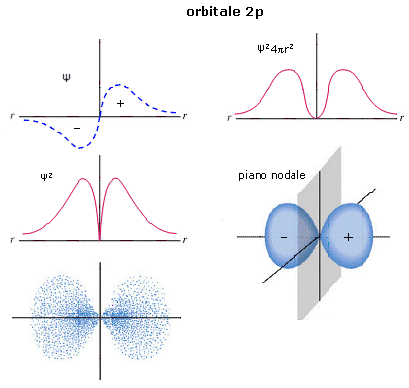
\includegraphics[scale=0.3]{distrib}
\end{figure}

Un ulteriore caratteristica delle distribuzioni di probabilità che deve essere rispettata anche dalla funzione d'onda di un sistema quantistico sta nel valore del suo integrale. Infatti se si considera tutto lo spazio di esistenza di una densità di probabilità allora il suo integrale deve dare come risposta la certezza di trovare l'oggetto analizzato, quindi l'integrale deve valere 1.
\begin{equation}
\int \Psi^* \Psi dr = \langle\Psi\vert\Psi\rangle=1
\end{equation}
 Tutte le affermazioni appena fatte si applicano alle funzioni d'onda di una singola particella ma anche a funzioni d'onda che descrivono il comportamento complessivo di $N$ particelle come gli orbitali molecolari. Tali funzioni saranno semplicemente definite come:
 \begin{equation}
 \Psi(r_1,r_2,r_3,\ldots,r_N,t)
 \end{equation}
\subsection{La definizione di uno stato quantistico} 
Per definire uno stato quantistico sono necessari due ingredienti:
\begin{itemize}
\item La funzione d'onda $\Psi$;
\item Un operatore $\hat{A}$.
\end{itemize}
Dato che la natura della funzione d'onda è già stata ampiamente esplorata, ci concentreremo ora sulle caratteristiche di un \emph{operatore}. Esso rappresenta un'\emph{osservabile} del sistema quantistico, quindi una variabile che ne definisce univocamente lo stato. Esempi di tali \emph{osservabili} sono l'\emph{energia}, la \emph{quantità di moto} e la \emph{posizione}.
Un operatore, affinchè descriva un'osservabile deve soddisfare alcune condizioni:
\begin{itemize}
\item Condizione di \emph{linearità}: $$\hat{A}[c_1\Psi_1+c_2\Psi_2]=c_1 \hat{A}\Psi_1 +c_2 \hat{A}\Psi_2 $$
\item Condizione di \emph{hermitianità}:
$$ \int f^*\hat{A}gd\tau=\int g\hat{A}^*f^*d\tau$$
\item Condizione del valore atteso coincidente con la media:
$$\langle A\rangle=\frac{\langle\Psi\vert\hat{A}\vert\Psi\rangle}{\langle\Psi\vert\Psi\rangle} $$ 
\end{itemize} 
Se queste condizioni sono verificate allora saranno valide anche le seguenti proprietà:
\begin{itemize}
\item Gli autovalori degli operatori sono \emph{reali};
\item Gli autovettori corrispondenti a diversi autovalori non degeneri sono ortogonali tra loro;
\item Se due operatori commutano allora è possibile misurare i loro autovalori con eguale precisione.
\end{itemize}

\subsection{Stati stazionari}
Definiamo gli \emph{stati stazionari} \index{stati stazionari} come quegli stati quantistici che \emph{non dipendono dal tempo}. Una tale definizione potrebbe essere controintuitiva, in quanto qualsiasi sistema reale ha un'intriseca dipendenza dal tempo. Tuttavia se si immagina di dividere il tempo in istanti allora è possibile "vedere" uno stato stazionario come la fotografia di uno stato del sistema in un preciso istante. In perfetta analogia, dato che si sta parlando di funzioni d'onda si può immaginare di lanciare un sasso in uno stagno per poi bloccare il tempo e osservare la \emph{forma d'onda}. Matematicamente una simile operazione si concretizza nel metodo della \emph{separazione delle variabili}.
A partire dall'equazione di Schr\"oedinger dipendente dal tempo si deduce che l'operatore \emph{hamiltoniano} non dipenda dalla variabile temporale:
\begin{equation}
\hat{H}\Psi(r,t)= \imath\hslash\frac{\partial\Psi(r,t)}{\partial t}
\end{equation}
con:
\begin{equation}
\hat{H}=\hat{T}+\hat{V} \Rightarrow \frac{\partial\hat{H}}{\partial t	}=0
\end{equation}
Poiché $\hat{T}$ e $\hat{V}$ sono l'energia \emph{cinetica} e l'energia \emph{potenziale}, e non includono nella forma funzionale una dipendenza dal tempo, in quanto parametri termodinamici, possiamo assumere che l'operatore \emph{hamiltoniano }agisca solo sulla parte spaziale della funzione d'onda, che possiamo quindi visualizzare come divisa in due parti:
\begin{equation}
\Psi(r,t)=\psi(r)f(t)
\end{equation}
Sostituendo questa nuova definizione di $\Psi$ nell'equazione di Schr\"oedinger dipendente dal tempo si ottiene:
\begin{equation}
\frac{1}{\psi(r)}\hat{H}\psi(r)=\frac{\imath \hslash}{f(t)}\frac{df(t)}{dt}
\end{equation}
Indicando come $E$ (energia) la costante di separazione si ottengono due equazioni:
\begin{equation}
\begin{aligned}
\hat{H}\psi(r)&=E\psi(r) \\ \\
\frac{df(t)}{dt} = (\imath \hslash)^{-1}Ef(t) &\rightarrow \frac{1}{\imath \hslash}\times\frac{\imath}{\imath}=-\frac{\imath}{\hslash} \\ \\
df(t) &= -\frac{\imath}{\hslash} Ef(t)dt \\ \\
f(t) &= e^{-\frac{\imath E t}{\hslash}}
\end{aligned}
\end{equation}
Da ciò si può costruire la forma funzionale della $\Psi$ dipendente dal tempo con le variabili spaziali separate da quelle temporali (Eq.\ref{sst}).
\begin{equation}
\label{sst}
\Psi(r,t)= \psi(r)e^{-\frac{\imath E t}{\hslash}}
\end{equation}
Se conosciamo la forma funzionale di una $\psi_n(r)$ (autovettore correlato all'autovalore $n$-$esimo$) allora possiamo determinarne la densità di probabilità:

\begin{equation}
\label{modde}
\begin{aligned}
\rvert\Psi_n(r,t)\rvert^2 d r &= \Psi_n(r,t)^{*} \Psi_n(r,t)dr \\ \\
&= \psi_n(r)^*e^{\frac{\imath E t}{\hslash}}\psi_n(r)e^{-\frac{\imath E t}{\hslash}} \\ \\
&= \psi_n(r)^*\psi_n(r) \\ \\
&=\rvert\psi_n(r)\rvert^2
\end{aligned}
\end{equation}
Si deduce quindi che la densità di probabilità sia indipendente dal tempo e che per valutare alcuni parametri, come l'energia, non sia necessario considerare la variabile temporale.

\section{L'approssimazione di Born-Oppenheimer}
Per capire matematicamente il significato dell'approssimazione di Born- Oppenheimer, \index{Born-Oppenheimer} dobbiamo, inizialmente definire l'operatore \emph{hamiltoniano totale non relativistico}, anche definito \emph{elettrostatico}. Consideriamo l'approssimazione non relativistica, in quanto gli elettroni che emergono dalla trattazione di Schr\"odinger non includono la coordinata di spin. Tale coordinata, insieme alla carica, definisce completamente l'elettrone. Tuttavia essa emerge naturalmente solo dalla trattazione \emph{relativistica }di \emph{Dirac}\index{Dirac}.
Non potendo risolvere l'equazione di Dirac a causa del costo computazionale, decisamente più elevato di Schr\"odinger, solitamente se necessario si includono gli effetti relativistici \emph{perturbando} un hamiltoniano non relativistico. Mentre lo spin viene aggiunto quando necessario moltiplicando $\psi$ per una funzione che descrive solo lo spin $\sigma$. Il fatto che l'hamitoniano sia elettrostatico, ci porta a non considerare l'annichilimento dell'elettrone con un positrone ovvero l'effetto dell'\emph{antimateria}.
In quest'ottica l'hamiltoniano diventa:
\begin{equation}
\begin{aligned}
\hat{H}_{tot}&=\hat{T}_n + \hat{H}_e +\hat{H}_{mp} \\
 \hat{H}_e &=\hat{T}_e + \hat{V}_{ne} +\hat{V}_{nn}+\hat{V}_{ee} \\ 
\hat{H}_{mp}&=-\frac{1}{2M_{tot}}\left(\sum \limits _{i} ^{N_{e^-}}\nabla _i \right)^2	 
\end{aligned}
\end{equation}
Dove $\hat{H}_{e}$ è l'hamiltoniano elettronico e $\hat{H}_{mp}$ è la \emph{polarizzazione di massa} ovvero un termine dovuto al fatto che è impossibile da separare il moto del centro di massa dai moti interni del sistema.
A questi termini si possono aggiungere altri elementi come il potenziale di interazione \emph{spin-orbita}, un potenziale \emph{esterno}, o dei potenziali utili alla descrizione di effetti che emergono solo in particolari spettroscopie.
Nell'approssimazione \emph{adiabatica} si considera la separazione delle funzioni d'onda nucleari rispetto \emph{una sola} funzione d'onda elettronica che considererà le coordinate nucleari come \emph{parametro}. Considerare un elettrone singolo semplifica notevolmente i calcoli:
\begin{equation}
\begin{aligned}
\Psi(R,r)&=\psi(r;R)\chi(R) \\
\hat{H}_{tot}\Psi(R,r)&=E_{tot}\Psi(R,r) \\
(\hat{T}_e + \hat{V}_{ne} +\hat{V}_{ee})\psi(r;R) &= E(R)\psi(r;R) \\
(\hat{T}_n + \hat{V}_{nn}+E(R))\chi(R)&= E_{tot}\chi(R)
\end{aligned}
\end{equation}
Nell'approssimazione di Born-Oppenheimer adiabatica ogni funzione d'onda viene calcolata singolarmente parametrizzata rispetto le funzioni nucleari. Ciò implica che le singole funzioni d'onda vedano il contributo degli altri elttroni come un \emph{campo medio}. Trascurando in questo modo le interazioni singole è possibile che in alcune regioni di spazio $2$ elettroni descritti da $2$ diverse funzioni d'onda abbiano energie paragonabili. Tali situazioni sono dette \emph{incroci evitati}\index{incroci evitati} e in tali regioni dello spazio le superfici di energia potenziale associate ad ogni funzione d'onda si possono quasi toccare (Fig.\ref{TonyNelly}). In una situazione simile l'energia dipenderà dalle coordinate elettroniche di $2$ elettroni e da $2$ set di parametri nucleari. Quindi l'approssimazione di Born-Oppenheimer adiabatica non è più valida e la descrizione che si ottiene applicandola è sbagliata.

\begin{figure}[H]
\centering
\caption{ Visualizzazione di due funzioni d'onda del sistema LiF con un incrocio evitato.}\label{TonyNelly}
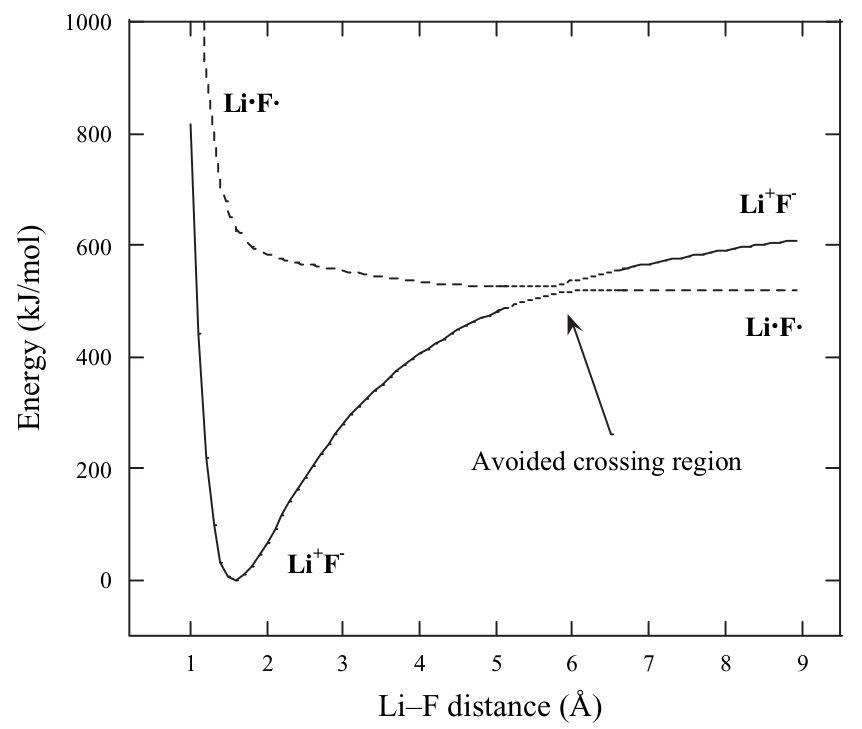
\includegraphics[scale=0.3]{ton}
\end{figure}
Se consideriamo che anche i \emph{nuclei} hanno una natura \emph{quantistica} allora risulta evidente che trascurando le loro funzioni d'onda otterremo una descrizione approssimata come campo medio di ogni proprietà molecolare dipendente dalla geometria. Ciò non genera alcun problema finché l'approssimazione di Born-Oppenheimer adiabatica resta valida, tuttavia in situazioni come gli incroci evitati, si renderà necessario considerare anche le funzioni d'onda nucleari. Dal momento che gli incroci evitati e altre situazioni analoghe si verificano molto di rado, una simile operazione non viene mai svolta.
\section{Metodi approssimati per risolvere l'equazione di Schr\"odinger}
L'equazione di Schr\"odinger può essere risolta analiticamente solo per un ristretto numero di sistemi \emph{monoelettronici}, come la molecola $H_{2}^+$. Quindi si renderà sempre necessaria l'adozione di un metodo approssimato (numerico). Le strategie possibili sono $2$:
\begin{itemize}
\item Metodo variazionale\index{metodo !variazionale};
\item Metodo perturbativo\index{metodo !perturbativo}.
\end{itemize}
Di seguito vengono analizzate entrambe dettagliatamente.
\subsection{Metodo variazionale e variazionale lineare}
Il metodo variazionale si basa sul \emph{teorema variazionale} e sul IV postulato della meccanica quantistica:
\begin{equation}
\label{crck}
\langle A\rangle=\frac{\langle\Psi\vert\hat{A}\vert\Psi\rangle}{\langle\Psi\vert\Psi\rangle} \Rightarrow\frac{\langle\Psi\vert\hat{H}\vert\Psi\rangle}{\langle\Psi\vert\Psi\rangle} = E[\Psi]\geq E_0
\end{equation}
E quindi:
\begin{equation}
\frac{\langle\Psi_0\vert\hat{H}\vert\Psi_0\rangle}{\langle\Psi_0\vert\Psi_0\rangle} = E_0
\end{equation}
In equazione \ref{crck} l'energia viene espressa come \emph{funzionale}, ovvero come un'applicazione che agendo su una funzione resituisce uno scalare ($\mathbb{R}^2\rightarrow\mathbb{R}$) esattamente come un'integrale definito.
Se non si ha a disposizione la funzione d'onda multielettronica esatta $\Psi$, come tipicamente accade, si deve far uso di una funzione approssimata che rispetti l'antisimmetria dei fermioni ($\Phi$) e che sia costituita dalle  funzioni d'onda dei singoli elettroni che costituiscono il sistema. Chiameremo queste funzioni d'onda monoelettroniche spin-orbitali $\phi$ definiti secondo LCAO mediante una combinazione lineare di funzioni atomiche $\chi$:
$$\phi=\varphi(r;R)\sigma (\alpha \vee \beta)$$
$$ \varphi=\sum \limits _i ^m c_i\chi_i $$
Dove $m$ è il massimo numero di funzioni atomiche utilizzate per descrivere le varie $\phi$. L'insieme \{$\chi_i$\} lo definiamo \emph{set base} e contiene tutte le funzioni generatrici dello spazio vettoriale in cui definiamo le funzioni d'onda monoelettroniche.
Una volta definita la funzione approssimata possiamo dedurre che la dipendenza lineare di questa dai parametri $\langle c\vert$ venga conservata anche nell'energia. Ovvero l'energia sarà un funzionale dei parametri $\langle c\vert$:
$$ E=E[\langle c\vert] $$
Se si esprime l'energia in questi termini allora il metodo viene definito \emph{variazionale lineare}.
La caratteristica principale di ogni metodo variazionale è che il risultato che si ottiene sarà sempre $\geq$ del valore vero. Ciò semplifica notevolmente i calcoli, infatti sarà sufficiente cercare i parametri per cui l'energia è minima per trovare la soluzione approssimata più vicina a quella reale. Per fare ciò si risolve una semplice equazione matriciale:
\begin{equation}
HC=SCE
\end{equation}
dove $H$ è la rappresentazione matriciale ($m\times m$) dell'operatore hamiltoniano ottenuta conoscendo il set base:
\begin{equation}
H_{\mu \nu}=\int \chi_{\mu}\hat{H}\chi_{\nu} d\tau
\end{equation}
Mentre $S$ è la matrice di sovrapposizione (Overlap) ($m\times m$), anch'essa definita a partire dal set base:
 
\begin{equation}
S_{\mu \nu}=\int \chi_{\mu}\chi_{\nu} d\tau
\end{equation}
Mentre $C$ è la matrice dei coefficienti della combinazione lineare ($m\times N_{e^-}$) ed $E$ è una matrice diagonale ($N_{e^-}\times N_{e^-}$) contenente gli autovalori associati a ogni singolo elettrone.

\subsection{Metodo perturbativo}
L'idea dietro i metodi perturbativi \index{metodo !perturbativo} consiste nel applicare una piccola perturbazione a un sistema in equilibrio, per poi studiare come il sistema reagisca a una tale perturbazione. L'assunzione più grande che si fa è che così come il sistema reagisce a una perturbazione di piccola entità così reagisce a una più importante in modo lineare. Come si può facilmente immaginare un tale comportamento potrebbe non essere sempre corretto, inficiando così la qualità dei risultati.
Nell'ambito della meccanica quantistica ciò viene svolto aggiungendo la perturbazione all'operatore hamiltoniano poiché esso è l'unica cosa che si conosce all'inizio di ogni calcolo, e definisce il sistema insieme alla funzione d'onda.
\begin{equation}
\label{lella}
\hat{H}=\hat{H}^0+\lambda\hat{H}'
\end{equation}
In equazione \ref{lella}, si scrive l'hamiltoniano come somma di due contributi:
\begin{itemize}
\item $\hat{H}^0$: Hamiltoniano imperturbato di cui si può calcolare esattamente autovalori e autofunzioni;
\item $\lambda\hat{H}'$: Perturbazione dell'hamiltoniano. Con $\lambda$ che determina l'intensità della perturbazione.
\end{itemize}
Al crescere dell'entità della perturbazione l'energia e la funzione d'onda variano in modo continuo, e la loro variazione rispetto $\lambda$ può essere espressa come serie di Taylor:
\begin{equation}
E_k=\lambda^0E_k^0+\lambda^1E_k^1+\lambda^2E_k^2+\ldots=\lambda^0E_k^0+\sum \limits
_{j=1}^{\infty} \lambda^jE_k^j
\end{equation}
\begin{equation}
\Psi_k=\lambda^0\Psi_k^0+\lambda^1\Psi_k^1+\lambda^2\Psi_k^2+\ldots=\lambda^0\Psi_k^0+\sum \limits
_{j=1}^{\infty} \lambda^j\Psi_k^j
\end{equation}
Dove i termini dopo quello imperturbato sono le correzioni perturbative ai diversi ordini.
Si può ora scrivere l'equazione di Schr\"odinger come:
\begin{equation}
\left(\hat{H}^0+\lambda\hat{H}'\right)\left(\lambda^0\Psi_k^0+\sum \limits
_{j=1}^{\infty} \lambda^j\Psi_k^j\right)=\left(\lambda^0E_k^0+\sum \limits
_{j=1}^{\infty} \lambda^jE_k^j\right)\left(\lambda^0\Psi_k^0+\sum \limits
_{j=1}^{\infty} \lambda^j\Psi_k^j\right)
\end{equation}
Portando a sinistra dell'uguale ed eguagliando tutto a $0$ si ottengono una serie di equazioni per i diversi valori di $\lambda$ le cui soluzioni esistono solo se $\lambda=0$ per qualsiasi ordine. Tali equazioni sono tutte del seguente tipo:
\begin{equation}
\label{pripryat}
\left(\hat{H}^0-E^0\right)\Psi_k^n+\hat{H}^1\Psi_k^{n-1}-\sum \limits
_{j=1}^{\infty}E_k^{n-j}\Psi_k^j=0
\end{equation}
Moltiplicando a sinistra per la funzione d'onda \emph{complessa coniugata} l'equazione \ref{pripryat} si riduce alla seguente forma:
\begin{equation}
\langle\Psi_k^0\vert\hat{H}^1\vert\Psi_k^{n-1}\rangle=E_k^n
\end{equation}
Quindi l'energia perturbativa al primo ordine può essere calcolata a partire dalla funzione d'onda imperturbata come segue:
\begin{equation}
E_k^1=\langle\Psi_k^0\vert\hat{H}^1\vert\Psi_k^{0}\rangle
\end{equation}
\section{La teoria di Hartree-Fock}
\subsection{La definizione della funzione d'onda multielettronica}
All'interno della teoria di Hartree-Fock dato che si considera un singolo elettrone in un campo medio generato dagli altri, risulta fondamentale definire l'energia associata a un singolo \emph{determinante di Slater} che diventerà la \emph{funzione d'onda multielettronica} che definisce lo stato fondamentale. \index{determinante di Slater} Per ottenere ciò conviene definire un operatore di \emph{antisimmetrizzazione}\index{antisimmetrizzazione} che agendo su un prodotto di Hartree degli spin-orbitali restituisca l'equivalente di un determinante di Slater:
\begin{equation}
\Phi^{HF}=\hat{A}\left[\prod \limits _{i=1} ^{N_{e^-}} \phi_i (i)\right]=\hat{A}\Pi
\end{equation}
Con:
\begin{equation}
\label{A}
\hat{A}= \frac{1}{\sqrt{N!}}\sum \limits_{p=0} ^{N_e-1} (-1)^p \hat{P}
\end{equation}
Dove l'operatore $\hat{P}$ genera tutte le possibili permutazioni di $2,3,4,\ldots$ coordinate elettroniche.
Si può dimostrare che per $A$ valgono le seguenti proprietà:
\begin{itemize}
\item $[A;H]=0$ ovvero $A$ commuta con l'hamiltoniano;
\item $AA=\sqrt{N!}A$ quindi $A$ è idempotente a meno di un fattore;
\item $\hat{A}=\hat{A}^{\dagger}$ quindi $A$ è hermitiano.
\end{itemize}
Costruendo la funzione d'onda multielettronica in questo modo si garatisce il comportamento corretto dell'\emph{antisimmetria}, infatti:
\begin{enumerate}
\item Lo scambio di due righe del determinante cambia il segno  della funzione d'onda. Ciò è corretto perché gli elettroni sono particelle \emph{fermioniche} pertanto antisimmettriche rispetto lo scambio:
$$\hat{P}_{ij}\Psi=-\Psi$$
Se questa condizione non fosse valida allora sarebbero particelle \emph{bosoniche};
\item La funzione d'onda molecolare soddisfa il principio di esclusione di Pauli, ovvero se nella matrice $C$ due colonne sono uguali il determinante si annulla. Equivalentemente si può dire che due elettroni identici occupano lo stesso \emph{spin-orbitale}\index{spin-orbitali} e ciò non avrebbe significato fisico;
\item La funzione d'onda rimane invariata se una riga viene moltiplicata per un qualsiasi multiplo;
\item La funzione d'onda è invariante rispetto a una \emph{trasformazione unitaria} degli spin orbitali.
\end{enumerate}
\subsubsection{L'introduzione dello spin} Al fine di dare una descrizione completa della funzione d'onda \emph{multielettronica} è necessario considerare anche il contributo dello spin. 
Tale contributo viene introdotto assumendo che si possano separare le variabili spaziali da quelle di spin, così facendo lo spin viene incluso in una funzione apposita ($\sigma_i$) che può assumere valori pari a $\pm\frac{1}{2}$. \\
Il problema principale che sorge da una simile trattazione è che in generale le autofunzioni dell'hamiltoniano potrebbero non essere autofunzioni dell'operatore \emph{momento di spin} $\hat{S}^2$.Infatti:
\begin{equation}
\begin{aligned}
\hat{S}^2 \Phi = \frac{1}{2}\left[ N+\frac{1}{2}(n_{\alpha}-n_{\beta})^2 \right]+\frac{1}{2}&\underbrace{\sum \limits_{i,j}\Phi_{ij}} \\
& \sigma_i\neq\sigma_j
\end{aligned}
\end{equation}
Le uniche $2$ possibilità affinché il determinante di Slater ($\Phi$) sia un'autofunzione dell'operatore momento di spin, si verificano quando gli elementi della sommatoria (i determinanti ottenuti scambiando gli \emph{stati di spin} degli spin-orbitali $i$ e $j$) si annullano o quando tali determinanti sono costanti. Queste due possibilità definiscono i confini di applicabilità del metodo di Hartree-Fock, che si limita ora a due casistiche ben definite:
\begin{itemize}
\item \textbf{Tutti gli spin-orbitali hanno lo stesso spin} ($n_{\alpha}=n_{\beta}$): Sono sistemi a \emph{guscio chiuso} con un numero pari di elettroni per cui vale: $$\hat{S}^2\Phi=0\Phi $$ Un sistema di questo tipo si definisce \emph{closed shell} e avendo $S=0$ la sua molteplicità di spin sarà $2S+1=1$, che definisce uno stato di \emph{singoletto}. Un metodo di Hartree-Fock che fa uso di questa definizione degli spin-orbitali viene definito \emph{Restricted Hartree-Fock}, \textbf{RHF}. La struttura elettronica si può visualizzare come in Fig.\ref{Rhf}.

\begin{figure}[H]
\centering
\caption{Struttura elettronica in un calcolo RHF.}\label{Rhf}
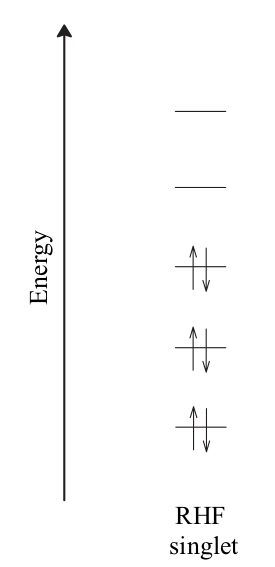
\includegraphics[scale=0.25]{rhf}
\end{figure}

\item \textbf{Non sono presenti elementi nella sommatoria} ($n_{\alpha}=N; n_{\beta}=0$): Se  la sommatoria contiene solo elementi nulli significa che i determinanti generati dallo scambio degli stati di spin di due spin-orbitali sono nulli, quindi tutti gli stati di spin sono identici. Ciò significa che si hanno solo spin-orbitali contenenti elettroni $\alpha$ o elettroni $\beta$. Questo è un problema perchè non è più possibile utilizzare un singolo determinante multi elettronico per descrivere $\Psi$ ma bisognerà utilizzarne uno contenente solo gli spin $\alpha$ e uno con solo gli spin $\beta$. Un metodo che faccia uso di una simile descrizione degli spin-orbitali si definisce \emph{Unrestricted Hartree-Fock}, \textbf{UHF} e la struttura elettronica è rappresentabile come in Fig.\ref{uhf}.

\begin{figure}[H]
\centering
\caption{Struttura elettronica in un calcolo UHF.}\label{uhf}
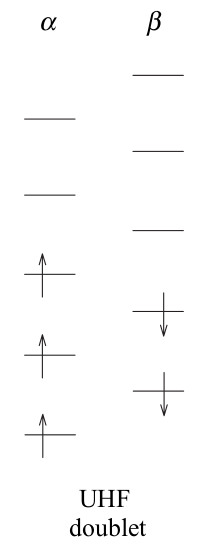
\includegraphics[scale=0.25]{uhf}
\end{figure}

In una simile struttura elettronica la molteplicità degli stati di spin è $2S+1=2$, quindi si ottiene uno stato di doppietto.
\end{itemize}
Per ovviare al problema del doppio determinante nel metodo \emph{UHF} si possono dividere gli elettroni in due set, uno con spin appaiati, e uno con spin paralleli. Entrambi i set descritti dallo stesso determinante.
Un metodo che faccia uso di una tale distribuzione degli spin si definisce \emph{Restricted Open Shell Hartree-Fock}, \textbf{ROHF}. Così facendo si mantiene lo stato di \emph{doppietto} e non si dividono gli elettroni accoppiati. La struttura elettronica associata a un simile metodo è riportata in Fig.\ref{Rof}.

\begin{figure}[H]
\centering
\caption{Struttura elettronica in un calcolo ROHF.}\label{Rof}
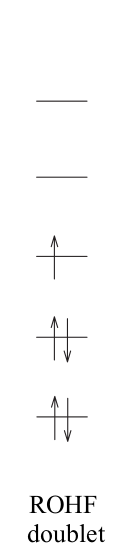
\includegraphics[scale=0.25]{rof}
\end{figure}
\subsection{La definizione dell'hamiltoniano}
Definiamo ora tutti i termini che costituiscono l'operatore hamiltoniano del metodo di Hartree-Fock:
\begin{equation}
\label{hamil}
\begin{aligned}
&\hat{H}_e=\hat{T}_e+\hat{V}_{ne}+\hat{V}_{ee}+\hat{V}_{nn} \\
&\ulcorner\text{Inizio termini monoelettronici} \urcorner\\
&\hat{T}_e=-\sum \limits_i ^{N_e} \frac{1}{2}\nabla^2_i \\
&\hat{V}_{ne}=-\sum \limits_A ^{N_n}\sum \limits_i ^{N_e} \frac{Z_A}{\vert R_A-r_i\vert}\\
&\llcorner \\
&\ulcorner\text{Inizio termini bielettronici} \urcorner\\
&\hat{V}_{ee}=\sum \limits_i ^{N_e}\sum \limits_{i>j} ^{N_e} \frac{1}{\vert r_i-r_j\vert}\\
&\llcorner\\
&\hat{V}_{nn}=\sum \limits_A ^{N_n}\sum \limits_{B>A} ^{N_n} \frac{Z_AZ_B}{\vert R_A-R_B\vert}
\end{aligned}
\end{equation}
Dividendo i termini dell'hamiltoniano in base al numero di elettroni che coinvolgono si intende dare un'interpretazione fisica ai diversi contributi dell'hamiltoniano:
\begin{itemize}
\item \textbf{Contributi monoelettronici}: Descrivono il moto di un singolo elettrone nel \emph{campo dei nuclei}:
\begin{equation}
h_i=-\frac{1}{2}\nabla^2_i-\sum \limits_A ^{N_n} \frac{Z_A}{\vert R_A-r_i\vert}
\end{equation}
\item \textbf{Contributi bielettronici}: Descrivono la repulsione \emph{coulombiana} tra elettroni:
\begin{equation}
g_{ij}=\frac{1}{\vert r_i-r_j\vert}
\end{equation}
\end{itemize}
Dato che il \emph{potenziale nucleare} è indipendente dalle coordinate dei nuclei esso viene considerato costante e integrato immediatamente:
\begin{equation}
\langle\Phi\vert V_{nn}\vert \Phi\rangle= V_{nn}\langle\Phi\vert\Phi\rangle = V_{nn}
\end{equation}
Il potenziale nucleare appena calcolato viene semplicemente sommato all'espressione dell'energia elettronica calcolabile come segue:
\begin{equation}
\begin{aligned}
E_{HF}&=\langle\Phi^{HF}\vert\hat{H}\vert\Phi^{HF}\rangle; \quad \Phi^{HF}=\hat{A}\Pi\\
&=\langle\hat{A}\Pi\vert\hat{H}\vert\hat{A}\Pi\rangle\\
&= \langle\Pi\vert\hat{A}^\dagger\hat{H}\hat{A}\vert\Pi\rangle \\
\text{Dato che vale: }[A;H]=0 \\
&= \langle\Pi\vert\hat{H}\hat{A}\hat{A}\vert\Pi\rangle\\
\text{Ricordando che: } AA=A\sqrt{N!} \\
&= \sqrt{N!}\langle\Pi\vert\hat{H}\hat{A}\vert\Pi\rangle
\end{aligned}
\end{equation}
Esplicitando ora la formulazione di $\hat{A}$ riportata in Eq.\ref{A}.
\begin{equation}
\begin{aligned}
E_{HF}&= \sqrt{N!}\langle\Pi\vert\hat{H}\vert\frac{1}{\sqrt{N!}}\sum \limits_{p=0} ^{N_e-1} (-1)^p \hat{P}\Pi\rangle \\
\text{Semplificando il fattore } \sqrt{N!} \\
&= \sum \limits_{p=0} ^{N_e-1} (-1)^p \langle \Pi\vert\hat{H}\vert\hat{P}\Pi\rangle \\
\text{Termine monoelettronico:} &= \sum \limits_{i=1} ^{N} \sum \limits_{p=0} ^{N_e-1} (-1)^p \langle \Pi\vert\hat{h}_i\vert\hat{P}\Pi\rangle + \\ \text{Termine bielettronico:} &+ \sum \limits_{j=1} ^{N} \sum \limits_{i=1} ^{N} \sum \limits_{p=0} ^{N_e-1} (-1)^p  \langle \Pi\vert\hat{g}_{ij}\vert\hat{P}\Pi\rangle + \\ \text{Potenziale nucleare:} &+V_{nn}
\end{aligned}
\end{equation}
Da quest'ultima equazione risulta evidente come l'energia elettronica dipenda dalla \emph{matrice di permutazione} che agisce sugli spin-orbitali che definiscono la funzione d'onda multielettronica monodeterminantale.
Si rende ora necessario definire una tale matrice. Possiamo assumere quindi che essa agisca solo in due modi:
\begin{itemize}
\item \textbf{Lascia invariato l'ordine degli spin-orbitali:}  $$\hat{P}=\hat{I}_n $$
\item \textbf{Cambia l'ordine degli spin-orbitali:}  $$\hat{P}=\hat{P}_{ij} $$
\end{itemize} 
Assumendo entrambe le definizioni di $\hat{P}$ si applicano ora consequenzialmente a una formulazione estesa delle funzioni d'onda multielettroniche sia per il termine monoelettronico che per quello bielettronico:\\
\subsubsection{Integrali monoelettronici}
\begin{itemize}
\item Analizziamo il primo caso ovvero $\hat{P}=\hat{I}_n $:
\begin{equation}
\begin{aligned}
\sum \limits_{i=1} ^{N}  \langle \Phi^{HF}\vert\hat{h}_i\vert\hat{P}\Phi^{HF}\rangle &= \langle\phi_1(r_1)\phi_2(r_2)\ldots \phi_n(r_n)\vert\hat{h}_i\vert\phi_1(r_1)\phi_2(r_2)\ldots \phi_n(r_n)\rangle \\
&= \underbrace{\langle\phi_1(r_1)\vert\phi_1(r_1)\rangle}_{\delta_{ij}=1} \ldots \langle\phi_i(r_i)\vert\hat{h}_i\vert\phi_i(r_i)\rangle \ldots \underbrace{\langle\phi_n(r_n)\vert\phi_n(r_n)\rangle}_{\delta_{ij}=1}\\
&= \langle\phi_i(r_i)\vert\hat{h}_i\vert\phi_i(r_i)\rangle = h_i
\end{aligned}
\end{equation}
Questo primo caso semplicemente coincide con il valore dell'integrale che quindi dovrà essere calcolato.
\item Analizziamo il secondo caso ovvero $\hat{P}=\hat{P}_{ij} $:
\begin{equation}
\begin{aligned}
&\sum \limits_{i=1} ^{N}  \langle \Phi^{HF}\vert\hat{h}_i\vert\hat{P}\Phi^{HF}\rangle = \\
&= \langle\phi_1(r_1)\ldots\phi_i(r_i),\phi_j(r_j)\ldots \phi_n(r_n)\vert\hat{h}_i\vert\phi_1(r_1)\ldots\phi_j(r_j),\phi_i(r_i)\ldots \phi_n(r_n)\rangle \\
&= \underbrace{\langle\phi_1(r_1)\vert\phi_1(r_1)\rangle}_{\delta_{ij}=1} \ldots \langle\phi_i(r_i)\vert\hat{h}_i\vert\phi_j(r_j)\rangle \ldots \underbrace{\langle\phi_i(r_i)\vert\phi_j(r_j)\rangle}_{\delta_{ij}=0}=0
\end{aligned}
\end{equation}
Nel caso in cui la permutazione avvenga allora l'integrale si annulla.
\end{itemize}



\subsubsection{Integrali bielettronici}
\begin{itemize}
\item Analizziamo il primo caso ovvero $\hat{P}=\hat{I}_n $ che coincide con il \emph{metodo di Hartree} senza il contributo di Fock:
\begin{equation}
\begin{aligned}
&\sum \limits_{i=1} ^{N}  \langle \Phi^{HF}\vert\hat{g}_{ij}\vert\hat{P}\Phi^{HF}\rangle = \\
&= \langle\phi_1(r_1)\ldots\phi_i(r_i),\phi_j(r_j)\ldots \phi_n(r_n)\vert\hat{g}_{ij}\vert\phi_1(r_1)\ldots\phi_i(r_i),\phi_j(r_j)\ldots \phi_n(r_n)\rangle \\
&= \underbrace{\langle\phi_1(r_1)\vert\phi_1(r_1)\rangle}_{\delta_{ij}=1} \ldots \underbrace{\langle\phi_i(r_i)\phi_j(r_j)\vert\hat{g}_{ij}\vert\phi_i(r_i)\phi_j(r_j)\rangle}_{J_{ij}= \text{Integrale coulombiano}} \ldots \underbrace{\langle\phi_n(r_n)\vert\phi_n(r_n)\rangle}_{\delta_{ij}=1} = J_{ij}
\end{aligned}
\end{equation}
Questo primo caso semplicemente coincide con il valore dell'integrale coulombiano che quindi dovrà essere calcolato.
\item Analizziamo il secondo caso ovvero $\hat{P}=\hat{P}_{ij} $ dove se $p=2k+1;\quad k\in \mathbb{N}$ allora $(-1)^p=-1$ quindi avremo un segno che rende negativo questo integrale:
\begin{equation}
\begin{aligned}
&\sum \limits_{i=1} ^{N}  \langle \Phi^{HF}\vert\hat{g}_{ij}\vert\hat{P}\Phi^{HF}\rangle = \\
&= \langle\phi_1(r_1)\ldots\phi_i(r_i),\phi_j(r_j)\ldots \phi_n(r_n)\vert\hat{g}_{ij}\vert\phi_1(r_1)\ldots\phi_j(r_j),\phi_i(r_i)\ldots \phi_n(r_n)\rangle \\
&= \underbrace{\langle\phi_1(r_1)\vert\phi_1(r_1)\rangle}_{\delta_{ij}=1} \ldots \underbrace{\langle\phi_i(r_i)\phi_j(r_j)\vert\hat{g}_{ij}\vert\phi_j(r_i)\phi_i(r_j)\rangle}_{K_{ij}= \text{Integrale di scambio}} \ldots \underbrace{\langle\phi_n(r_n)\vert\phi_n(r_n)\rangle}_{\delta_{ij}=1} = -K_{ij}
\end{aligned}
\end{equation}
Nel caso in cui la permutazione avvenga allora bisogna calcolare il valore dell'integrale di scambio e porlo negativo a causa dell'effetto dell'operatore permutazione. Uno dei contributi più importanti di Fock a questo metodo, dopo l'introduzione del determinante di Slater, è proprio l'introduzione dell'\emph{integrale di scambio}.
\end{itemize}
Dal momento che si sta considerando l'interazione di $2$ elettroni si deve introdurre nelle precedenti equazioni anche il contributo delle funzioni di spin che costituiscono gli spin-orbitali $\phi_i=\phi_i(r_i)\sigma_i(\alpha \vee \beta)$. Dal momento che è possibile separare le variabili di spin da quelle spaziali allora possiamo moltiplicare i contributi dello spin ai valori degli integrali calcolati:
\begin{itemize}
\item Integrale coulombiano:
\begin{equation}
J_{ij}=J_{ij} \underbrace{\langle\sigma_i\vert\sigma_i\rangle}_1 \underbrace{\langle\sigma_j\vert\sigma_j\rangle}_1
\end{equation}
Questo significa che questo integrale avrà sempre un valore non nullo, senza alcuna restrizione di spin. Questo è fisicamente corretto in quanto l'integrale coulombiano descrive la repulsione elettrostatica tra due elettroni, che è sempre presente. Infatti se due elettroni occupano lo stesso spazio e hanno lo stesso spin la loro distribuzione di probabilità sarà nulla ed essi saranno inevitabilmente lontani, quindi la loro interazione coulombiana sarà minima. Questa situazione risulta evidente se si prova a visualizzare le \emph{distribuzioni di probabilità} rispetto lo spazio. In un tale grafico si vedrà una \emph{buca} detta \emph{di Fermi} in corrispondenza dello $0$ di probabilità di trovare i due elettroni (Fig.\ref{Fer}).


\begin{figure}[H]
\centering
\caption{Buca di Fermi.}\label{Fer}
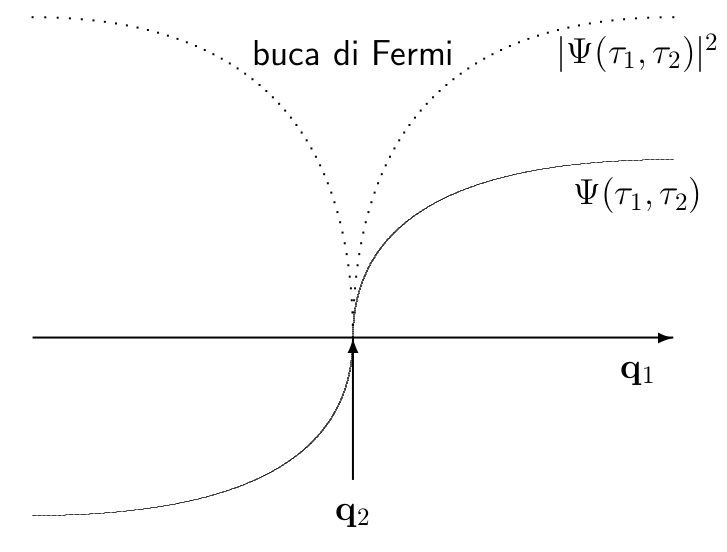
\includegraphics[scale=0.3]{fer}
\end{figure}

Il metodo di Hartree-Fock non riesce a descrivere con una buca la situazione in cui gli spin sono opposti, quindi per cui ci sia attrazione tra gli spin e repulsione tra le cariche. Tuttavia una descrizione tale esiste nei metodi post-HF e DFT dove viene definita \emph{buca di Coulomb}
\item Integrale di scambio:
\begin{equation}
K_{ij}=K_{ij} \underbrace{\langle\sigma_i\vert\sigma_j\rangle}_{\delta_{ij} }\underbrace{\langle\sigma_j\vert\sigma_i\rangle}_{\delta_{ij}}
\end{equation}
Quindi l'integrale di scambio dipenderà dall'orientazione degli spin:
\begin{itemize}
\item \textbf{Spin opposti}, $\sigma_i\neq \sigma_j$: $$K_{ij}=0$$
In questo caso i due spin opposti danno un'interazione attrattiva, tuttavia essa non viene considerata dall'integrale di scambio. Questo è uno dei principali contributi all'energia di correlazione statica che non viene considerata dal metodo HF;
\item \textbf{Spin paralleli}, $\sigma_i= \sigma_j$: $$K_{ij}\neq 0$$
\end{itemize}
Questo comportamento si può riassumere come una delta di Kronecker che impone delle restrizioni di spin all'integrale di scambio:$$ \delta_{\sigma_i \sigma_j}$$
\end{itemize}
Possiamo ora scrivere una formulazione completa dell'energia elettronica come funzione di un singolo determinante di Slater:
\begin{equation}
E^{HF}=\sum \limits_{i=1} ^{N}  \hat{h}_{i} + \sum \limits_{i=1} ^{N} \sum \limits_{j>i} ^{N}  (J_{ij}-K_{ij}\delta_{\sigma_i \sigma_j})+\langle V_{nn}\rangle
\end{equation}
Aggiungendo la possibilità che ogni elettrone possa interagire con sè stesso, i termini all'interno della sommatoria raddoppiano pertanto bisogna moltiplicare tutto per $\frac{1}{2}$. Ciò non inficia il calcolo poiché i termini di scambio annullano i termini di autointerazione coulombiana senza significato fisico.
 \begin{equation}
E^{HF}=\sum \limits_{i=1} ^{N}  \hat{h}_{i} + \frac{1}{2} \sum \limits_{i=1} ^{N} \sum \limits_{j=1} ^{N}  (J_{ij}-K_{ij}\delta_{\sigma_i \sigma_j})+\langle V_{nn}\rangle
\end{equation}

\subsubsection{Definizione degli elementi delle matrici di coulomb e di scambio} Riscriviamo ora gli integrali in termini di un singolo orbitale, omettendo le funzioni di spin in quanto contribuiscono come delta di Kronecker. In questo modo possiamo definire tali integrali in termini di orbitali dipendenti da una \emph{singola} coordinata elettronica.
 \begin{equation}
 \begin{aligned}
J_{ij}&=\langle\phi_i(r_i) \phi_j(r_j)\vert\frac{1}{r_{ij}}\vert\phi_i(r_i) \phi_j(r_j)\rangle  \\
&= \int \int \phi_i^*(r_i) \phi_j^*(r_j)\frac{1}{r_{ij}}    \phi_i(r_i) \phi_j(r_j) dr_i dr_j \\
&\text{Ricordando che }\phi_i^*(r_i)\phi_i(r_i)dr_i =\vert\phi_i(r_i)\vert^2	 \\
&\text{E che non possiamo invertire l'ordine delle moltiplicazioni}\\
&= \int \int \frac{\vert\phi_i(r_i)\vert^2\vert\phi_j(r_j)\vert^2}{r_{ij}}dr_i dr_j \\
&= \int \vert\phi_i(r_i)\vert^2dr_i \int \frac{\vert\phi_j(r_j)\vert^2}{r_{ij}}dr_j \\
&=\langle\phi_i(r_i)\vert\underbrace{\langle\phi_j(r_j)\vert\frac{1}{r_{ij}}\vert\phi_j(r_j)\rangle}_{J_j=\text{Operatore locale}}\vert\phi_i(r_i)\rangle
 \end{aligned}
\end{equation}
Da questa derivazione emerge che l'operatore coulombiano è un \emph{operatore locale} ovvero un operatore che dipende esclusivamente dalla coordinata spaziale di un solo elettrone. Infatti per costruire il suo elemento di matrice non è necessaria più di $1$ orbitale.

 \begin{equation}
 \begin{aligned}
K_{ij}&=\langle\phi_i(r_i) \phi_j(r_j)\vert\frac{1}{r_{ij}}\vert \phi_j(r_j)\phi_i(r_i)\rangle  \\
&= \int \int \phi_i^*(r_i) \phi_j^*(r_j)\frac{1}{r_{ij}}  \phi_j(r_j)\phi_i(r_i) dr_i dr_j \\
&\text{Ricordando che non possiamo invertire} \\ &\text{l'ordine delle moltiplicazioni}\\
&= \int \phi_i^*(r_i)\phi_j(r_j)dr_idr_j \int \frac{\phi_j^*(r_j)\phi_i(r_i)}{r_{ij}}dr_idr_j \\
&=\langle\phi_i(r_i)\vert\underbrace{\langle\phi_j(r_j)\vert\frac{1}{r_{ij}}\vert\phi_i(r_i)\rangle}_{K_j=\text{Operatore non locale}}\vert\phi_j(r_j)\rangle
 \end{aligned}
\end{equation}
 In questo caso si nota che l'integrale di scambio è un  \emph{operatore non locale} ovvero un'opearatore che dipende simultaneamente dalle coordinate spaziali di $2$ elettroni.
 \subsection{La minimizzazione dell'energia con il metodo variazionale}
 Al fine di valutare quale sia la migliore funzione monodeterminantale in grado di descrivere l'energia del sistema in senso variazionale, proviamo ora a ricavare un'espressione per la variazione di energia necessaria a eseguire un passo di minimizzazione, ovvero un'espressione per la \emph{stazionarietà dell'energia } rispetto ad arbitrarie variazioni degli spin-orbitali.
 \begin{equation}
 \frac{\partial E}{\partial \phi_i}=0
 \end{equation}
Gli spin orbitali non sono, tuttavia, liberi di variare liberamente, infatti resta valido il vincolo che i determinanti di Slater multi-elettronici che sono \emph{autovettori} dell'hamiltoniano, siano tra loro \emph{ortogonali}. Questa condizione è il vincolo che dobbiamo imporre alla variazione degli spin-orbitali. Per attuare una procedura di minimizzazione \emph{con vincoli} e necessario appoggiarsi al \emph{metodo di Lagrange}\index{Lagrange !metodo di}, tipico della meccanica razionale.
Il primo passaggio è costruirsi una funzione che descriva l'energia a meno dei vincoli imposti, in modo che tali vincoli non generino variazioni sostanziali dell'energia. Tale funzione prende il nome di \emph{lagrangiana}:
\begin{equation}
\mathcal{L}=E-\underbrace{\sum \limits _{ij} ^{N_e}\lambda _{ij} (\langle\phi_i\vert\phi_j\rangle-\delta_{ij})}_{\text{condizione di ortogonalità}}
\end{equation}
Se la \emph{condizione di ortogonalità} non è rispettata allora $\langle\Phi_i\vert\Phi_i\rangle\neq0$ e $delta_{ij}=0$, quindi la sommatoria dei \emph{moltiplicatori di Lagrange} risulta essere $\neq 0$ e l'energia subisce una modifica sostanziale al variare degli orbitali.
Se, invece, la condizione di ortogonalità è verificata il termine tra parentesi si annulla e l'energia non varia al variare degli orbitali, quindi minimizzare la \emph{Lagrangiana} corrisponde a minimizzare l'energia.
Andiamo ora a porre a $0$ la variazione della \emph{Lagrangiana} rispetto la variazione degli orbitali molecolari, assumiamo quindi che i termini nella sommatoria varino linearmente con la variazione dell'energia. Se ciò avviene allora stiamo minimizzando la lagrangiana:
\begin{equation}
\label{diofa}
\begin{aligned}
 \delta\mathcal{L}&= \delta E-\sum \limits _{ij} ^{N_e}\lambda _{ij} (\langle \delta \phi_i\vert\phi_j\rangle+\langle\Phi_i\vert\delta\Phi_j\rangle)=0
\end{aligned}
\end{equation}
Dobbiamo ora definire i termini che appaiono in Eq.\ref{diofa}:
\begin{equation}
\begin{aligned}
\delta E &= \sum \limits_{i=1} ^{N_e}( \langle\delta \phi_i\vert \hat{h}_{i}\vert\phi_i\rangle +\langle\phi_i\vert\hat{h}_i\vert\delta\phi_i\rangle ) \\ &+ \frac{1}{2} \sum \limits_{i=1} ^{N_e} \sum \limits_{j=1} ^{N_e} \underbrace{\langle\delta\phi_i\vert(J_{j}-K_{j})\vert\phi_i\rangle}_A   + \underbrace{\langle\phi_i\vert(J_{j}-K_{j})\vert\delta\phi_i\rangle}_B \\
&+\underbrace{\langle\delta\phi_i\vert(J_{i}-K_{i})\vert\phi_i\rangle}_{A'} + \underbrace{\langle\phi_i\vert(J_{i}-K_{i})\vert\delta\phi_i\rangle}_{B'}
\end{aligned}
\end{equation}
Dal momento che $$ A=A' $$ e $$B = B'$$ possiamo raccogliere entrambe moltiplicare tutto per $2$, eliminando così il fattore $1/2$ che moltiplica la sommatoria:
\begin{equation}
\begin{aligned}
\delta E &= \sum \limits_{i=1} ^{N_e}( \langle\delta \phi_i\vert \hat{h}_{i}\vert\phi_i\rangle +\langle\phi_i\vert\hat{h}_i\vert\delta\phi_i\rangle ) \\ &+ \sum \limits_{i=1} ^{N_e} \sum \limits_{j=1} ^{N_e} \langle\delta\phi_i\vert(J_{j}-K_{j})\vert\phi_i\rangle   + \langle\phi_i\vert(J_{j}-K_{j})\vert\delta\phi_i\rangle \\
&\text{Riscriviamo tutto in termini di un nuovo operatore: } \hat{F}_i \\
\delta E &=\sum \limits_{i=1} ^{N_e}( \langle\delta \phi_i\vert \hat{F}_i\vert\phi_i\rangle +\langle\phi_i\vert\hat{F}_i\vert\delta\phi_i\rangle ) \\
&\hat{F}_i=\hat{h}_i+ \sum \limits_{j=1} ^{N_e}(J_{j}-K_{j})
\end{aligned}
\end{equation}
Il nuovo operatore appena ottenuto prende il nome di  \emph{operatore di Fock} \index{operatore di Fock} ed associato alla \emph{variazione di energia} e non all'energia stessa, infatti descrive le variazioni di energia cinetica dovute all'attrazione dei nuclei  e alla repulsione degli altri elettroni.
Inserendo ora la definizione appena data di $\delta E$ in Eq.\ref{diofa} e passando dall'\emph{ortogonalità} degli orbitali a quella degli spin-orbitali(operazione lecita perchè vale la separazione delle variabili di spin, quindi se sono ortogonali gli orbitali molecolari lo devono essere anche gli spin orbitali che li costituiscono), si ottiene:
\begin{equation}
\label{cacca}
\begin{aligned}
\delta\mathcal{L}&= \sum \limits_{i=1} ^{N_e}( \langle\delta \phi_i\vert \hat{F}_i\vert\phi_i\rangle +\langle\phi_i\vert\hat{F}_i\vert\delta\phi_i\rangle )-\sum \limits _{ij} ^{N_e}\lambda _{ij} (\langle \delta \phi_i\vert\phi_j\rangle+\langle\phi_i\vert\delta\phi_j\rangle)=0\\
&= \sum \limits_{i=1} ^{N_e}( \langle\delta \phi_i\vert \hat{F}_i\vert\phi_i\rangle-\sum \limits _{ij} ^{N_e}\lambda _{ij} \langle \delta \phi_i\vert\phi_j\rangle + \sum \limits_{i=1} ^{N_e}( \langle\delta \phi_i\vert \hat{F}_i\vert\phi_i\rangle^*-\sum \limits _{ij} ^{N_e}\lambda _{ij} \langle \delta \phi_i\vert\phi_j\rangle^*
\end{aligned}
\end{equation}
Dato che deve valere $\delta\mathcal{L}=0$ allora :
\begin{equation}
\sum \limits_{i=1} ^{N_e}( \langle\delta \phi_i\vert \hat{F}_i\vert\phi_i\rangle-\sum \limits _{ij} ^{N_e}\lambda _{ij} \langle \delta \phi_i\vert\phi_j\rangle =\left(  \sum \limits_{i=1} ^{N_e}( \langle\delta \phi_i\vert \hat{F}_i\vert\phi_i\rangle^*-\sum \limits _{ij} ^{N_e}\lambda _{ij} \langle \delta \phi_i\vert\phi_j\rangle^*\right)^*
\end{equation}
Quindi il primo e il terzo termine si possono semplificare e l'equazione si riduce a:
\begin{equation}
\sum \limits _{ij} ^{N_e}(\lambda^*_{ji}-\lambda_{ij})\langle \delta \phi_i\vert\phi_j\rangle = 0
\end{equation}
Una simile uguglianza si può soddisfare solo se $\lambda_{ij}=\lambda^*_{ji}$, ovvero se i \emph{moltiplicatori di Lagrange }sono gli elementi di una matrice \emph{hermitiana}. Si può quindi pensare di riscrivere in termini matriciali l'equazione \ref{cacca} non più come uguaglianza a $0$ ma esplicitando l'operatore di Fock e la matrice dei moltiplicatori di Lagrange:
\begin{equation}
\hat{F}_i \phi_i= \sum \limits_{j=1} ^{N_e}\lambda_{ij} \phi_j
\end{equation}
Se si trova una \emph{trasformazione unitaria} che diagonalizza la matrice contenente $\lambda_{ij}$ allora si può riscrivere questa equazione come un'equazione agli \emph{pseudo-autovalori}:
\begin{equation}
U^{-1} \Lambda U = \mathcal{E}
\end{equation}
\begin{equation}
\hat{F}_i \phi_i'= \varepsilon_i \phi_i'
\end{equation}
Questi orbitali che si ottengono sono degli orbitali molecolari multielettronici che definiamo \emph{canonici} e i \emph{moltiplicatori di Lagrange} acquisiscono il significato fisico di energie degli orbitali molecolari, mentre gli autovettori che si ottengono diagonalizzando la matrice di Fock sono anche detti orbitali SCF \emph{Self Consistent Field} e sono la miglior combinazione di orbitali molecolari monoelettronici ortogonali tra loro, che rende minima l'energia.
L'energia totale del sistema, tuttavia non può essere vista come una mera somma delle energie degli orbitali molecolari e sarà, quindi descrivibile come:
\begin{equation}
E_{tot}=\sum \limits_{i=1} ^{N_e}  \varepsilon_{i} + \frac{1}{2} \sum \limits_{ij} ^{N_e}  (J_{ij}-K_{ij}\delta_{\sigma_i \sigma_j})+\langle V_{nn}\rangle
\end{equation}
\section{Il teorema di Koopman}
Con \emph{teorema di Koopman} si intende l'espressione dell'energia di ionizzazione di una molecola calcolata come differenza tra le energie di \emph{Hartree-Fock} del sistema in stato fondamentale e lo stesso sistema privato di un elettrone:
\begin{equation}
\begin{aligned}
E^{N}&=\sum \limits_{i=1} ^{N}  \hat{h}_{i} + \frac{1}{2} \sum \limits_{i=1} ^{N} \sum \limits_{j=1} ^{N}  (J_{ij}-K_{ij})+\langle V_{nn}\rangle \\
E^{N-1}&=\sum \limits_{i=1} ^{N-1}  \hat{h}_{i} + \frac{1}{2} \sum \limits_{i=1} ^{N-1} \sum \limits_{j=1} ^{N-1}  (J_{ij}-K_{ij})+\langle V_{nn}\rangle \\
E^{N}-E^{N-1}&= \hat{h}_{k}+\frac{1}{2} \sum \limits_{i=1} ^{N}  (J_{ik}-K_{ik})+\frac{1}{2} \sum \limits_{j=1} ^{N}  (J_{kj}-K_{kj})\\
&=\hat{h}_{k}+ \sum \limits_{j=1} ^{N}  (J_{kj}-K_{kj})= \varepsilon_k
\end{aligned}
\end{equation}
Dal momento che le matrici di coulomb e scambio sono costruite sullo stesso set di orbitali (autovettori della matrice di Fock) per entrambe le energie, si sta implicitamente assumendo che gli orbitali molecolari non cambino forma al variare dell'energia. Ovviamente questa assunzione è assurda, ma per piccole variazioni di energia si può approssimare come valida.
Da questa trattazione emerge che l'energia di ionizzazione coincide con l'energia dell'orbitale che viene ionizzato nell'ipotesi che l'estrazione dell'elettrone avvenga in $2$ passaggi ovvero:
\begin{itemize}
\item Rimozione dell'elettrone senza perturbazione della densità elettronica;
\item Riarrangiamento della densità elettronica.
\end{itemize} 
Si potrebbe pensare di applicare lo stesso ragionamento all'affinità elettronica ma bisognerebbe coinvolgere orbitali viruali che non sono definiti in un processo di calcolo HF (SCF)
\section{Approssimazione del set base}
Fin'ora tutti gli orbitali considerati nei calcoli sono stati definiti come \emph{spin-orbitali} \index{spin-orbitali} monoelettronici, che se considerati tutti insieme mediante un determinante di Slater danno come risultato la funzione d'onda multielettronica molecolare. Tuttavia quando si prepara l'input di un programma di chimica computazionale oltre alla geometria si fornisce anche il \emph{set base}. Ovvero un insieme più o meno ampio di funzioni che vengono paragonate a \emph{orbitali atomici} e che combinate linearmente generano gli orbitali molecolari utilizzati nei calcoli della teoria Hartree-Fock. La scelta di quali funzioni utilizzare per fare ciò deve essere guidata da $2$ criteri:
\begin{itemize}
\item Il comportamento di tali funzioni deve essere coerente con la fisica del sistema analizzato;
\item La funzione scelta deve essere semplice da integrare.
\end{itemize}
L'approccio del set base è preponderante, sebbene alcuni programmi facciano uso di metodi HF \emph{numerici}, in cui la forma degli orbitali molecolari viene valutata numericamente, campionando in determinati punti griglia dello spazio il valore assunto dalla funzione d'onda stessa. Contrariamente ai metodi numerici, l'utilizzo di un set base per costruire gli orbitali molecolari si giustifica agevolmente considerando valido l'approccio LCAO. Infatti le funzioni generatrici vengono equiparate agli orbitali atomici e gli orbitali molecolari sono costruiti come segue:
\begin{equation}
\phi_i= \sum \limits_{\mu = 1}^m c_{\mu i }\chi_{\mu} (r-R_A)
\end{equation}
Il termine tra parentesi definisce per ogni atomo un'insieme di funzioni base e posiziona le funzioni appartenenti a tale atomo sull'atomo stesso.
Nella sezione sulla teoria di Hartree-Fock abbiamo trovato un insieme di orbitali molecolari che rendono minima l'energia del sistema, tuttavia non avendo una definizione degli orbitali in termini del set base risultava difficile comprendere quali funzioni utilizzare per definire le matrici di Coulomb e di scambio e, conseguentemente, quella di Fock. Ora andiamo a vedere come si possa partire dalle funzioni del set base per costruirsi tali funzioni:
\begin{equation}
\begin{aligned}
\hat{F}_i(r) \phi_i(r)&= \varepsilon_i\phi_i(r) \\
\hat{F}_i(r)\sum \limits_{\mu = 1}^m c_{\mu i }\chi_{\mu}&= \varepsilon_i\sum \limits_{\mu = 1}^m c_{\mu i }\chi_{\mu}\\
\text{Moltiplicando a sinistra per: } \chi^*_{\mu} \\
\langle \chi_{\mu}\vert \hat{F}_i\vert\sum \limits_{\nu = 1}^m c_{\nu i }\chi_{\nu}\rangle &= \varepsilon_i \langle \chi_{\mu}\vert\sum \limits_{\nu = 1}^m c_{\nu i }\chi_{\nu}\rangle\\
\sum \limits_{\nu = 1}^m c_{\nu i }\underbrace{\langle \chi_{\mu}\vert \hat{F}_i\vert\chi_{\nu}\rangle}_{\text{Elemento di matrice }F_{\mu \nu} } &= \varepsilon_i \sum \limits_{\nu = 1}^m c_{\nu i }\underbrace{\langle \chi_{\mu}\vert\chi_{\nu}\rangle}_{\text{Elemento di matrice: } S _{\mu \nu}}
\end{aligned}
\end{equation}
In termini matriciali si può esprimere questo risultato aggiungendo il vincolo dell'ortonrmalità come:
\begin{equation}
\biggr \{ 
\begin{aligned}
FC = SCE \\
C^{\dagger}SC=I
\end{aligned}
\end{equation}
Queste prendono il nome di \emph{equazioni di Roothaan-Hall}\index{Roothaan-Hall !equazioni di} e sono le equazioni di Hartree-Fock trasposte nella base degli orbitali atomici.
Per avere una descrizione completa di queste equazioni occorre definire in termini di set base i singoli operatori che costituisono l'operatore di Fock:
\begin{equation}
\begin{aligned}
\langle \chi_{\mu}\vert \hat{F}_i\vert\chi_{\nu}\rangle &= \langle \chi_{\mu}\vert \hat{h}_i\vert\chi_{\nu}\rangle + \sum \limits _{j} ^{MO_{occ.}}\langle \chi_{\mu}\vert J_j-K_j\vert\chi_{\nu}\rangle\\
&= \langle \chi_{\mu}\vert \hat{h}_i\vert\chi_{\nu}\rangle + \sum \limits _{j} ^{MO_{occ.}}\langle\chi_{\mu}\phi_j\vert g \vert\chi_{\nu}\phi_j\rangle-\langle\chi_{\mu}\phi_j\vert g \vert\phi_j\chi_{\nu}\rangle\\
&= \langle \chi_{\mu}\vert \hat{h}_i\vert\chi_{\nu}\rangle + \sum \limits _{j} ^{MO_{occ.}}\sum \limits _{\gamma \delta} ^{m}c_{\gamma j} c_{\delta j}(\langle\chi_{\mu}\chi_{\gamma}\vert g \vert\chi_{\nu}\chi_{\delta}\rangle-\langle\chi_{\mu}\chi_{\gamma}\vert g \vert\chi_{\delta}\chi_{\nu}\rangle)\\
&\text{Definiamo: } D_{\gamma\delta }=\sum \limits _{j} ^{MO_{occ.}}c_{\gamma j} c_{\delta j} \\
&= \langle \chi_{\mu}\vert \hat{h}_i\vert\chi_{\nu}\rangle + \sum \limits _{\gamma \delta} ^{m}D_{\gamma\delta }(\underbrace{\langle\chi_{\mu}\chi_{\gamma}\vert g \vert\chi_{\nu}\chi_{\delta}\rangle}_{J_{\gamma\delta }}-\underbrace{\langle\chi_{\mu}\chi_{\gamma}\vert g \vert\chi_{\delta}\chi_{\nu}\rangle}_{K_{\gamma\delta }})\\
\end{aligned} 
\end{equation}
In questa equazione abbiamo definito una nuova matrice $D_{\gamma\delta }$ che chiamiamo \emph{matrice di densità}; essa contiene i coefficienti che vanno a definire gli orbitali molecolari in termini degli orbitali atomici. Sarà quindi la matrice sulla quale, per mezzo dei moltiplicatori di Lagrange, verrà minimizzata l'energia variazionale.
L'espressione dell'energia elettronica minima in senso variazionale ricavata con il metodo di Lagrange, espressa  in termini del set base diventa dunque:
\begin{equation}
\begin{aligned}
E&=\sum \limits_{i=1} ^{N}\sum \limits _{\mu \nu} ^{m}c_{\mu i} c_{\nu i} \langle\chi_{\mu}\vert \hat{h}_{i}\vert\chi_{\nu}\rangle + \\
&+ \frac{1}{2} \sum \limits_{i=1} ^{N} \sum \limits_{j=1} ^{N} \sum \limits _{\mu \nu} ^{m} c_{\mu i} c_{\gamma j}c_{\nu i} c_{\delta j}(\langle\chi_{\mu}\chi_{\gamma}\vert g \vert\chi_{\nu}\chi_{\delta}-\langle\chi_{\mu}\chi_{\gamma}\vert g \vert\chi_{\delta}\chi_{\nu}\rangle) +V_{nn}\\
&=\sum \limits _{\mu \nu} ^{m}D_{\mu \nu} \langle\chi_{\mu}\vert \hat{h}_{i}\vert\chi_{\nu}\rangle + \frac{1}{2}  \sum \limits _{\mu \nu} ^{m} D_{\mu \nu} D_{\gamma \delta}(\langle\chi_{\mu}\chi_{\gamma}\vert g \vert\chi_{\nu}\chi_{\delta}-\langle\chi_{\mu}\chi_{\gamma}\vert g \vert\chi_{\delta}\chi_{\nu}\rangle) +V_{nn} \\
&= \sum \limits _{\mu \nu} ^{m}D_{\mu \nu}\hat{h}_{\mu \nu} + \frac{1}{2}  \sum \limits _{\mu \nu} ^{m}( D_{\mu \nu} D_{\gamma \delta}- D_{\mu \delta} D_{\gamma \nu})\underbrace{\langle\chi_{\mu}\chi_{\gamma}\vert g \vert\chi_{\nu}\chi_{\delta}\rangle}_{\text{Integrale bielettronico}} +V_{nn}
\end{aligned}
\end{equation}
In questa equazione gli integrali bielettronici sono stati unificati in modo da mantenere una dipendenza diretta tra l'energia elettronica e la matrice di densità. Così facendo si può ricavare facilmente l'energia calcolando esclusivamente un \emph{integrale monoelettronico} e un \emph{integrale bielettronico} e conoscendo una stima dei coefficienti delle combinazioni lineari che definiscono gli orbitali molecolari.
Gli integrali sono calcolabili analiticamente:
\begin{equation}
h_{\mu \nu}= \int \chi_\mu (r_1)\left(-\frac{1}{2}\nabla^2\right) \chi_\nu(r_1) dr_1 + \sum \limits_a ^{N_n} \int \chi_\mu (r_1)\left(\frac{Z_a}{\vert R_a-r_1\vert}\right)\chi_\nu(r_1) dr_1
\end{equation}
\begin{equation}
\langle\chi_{\mu}\chi_{\gamma}\vert g \vert\chi_{\nu}\chi_{\delta}\rangle= \int \chi_\mu (r_1) \chi_\gamma(r_2)\left(\frac{1}{\vert r_1-r_2\vert}\right)\chi_{\nu}(r_1)\chi_{\delta}(r_2) dr_1 dr_2 
\end{equation}
A questo punto si può procedere iterativamente alla ricerca dei coefficienti migliori in grado di descrivere gli orbitali molecolari:
\begin{enumerate}
\item Stima iniziale della matrice di densità;
\item Calcolo degli integrali mono- e bi-elettronici;
\item Definizione della matrice di Fock;
\item Diagonalizzazione della matrice di Fock con l'equazioni di Roothaan-Hall;
\item Ridefinizione della matrice densità in termini dei coefficienti risultanti dalla diagonalizzazione;
\item Ricominciare dal punto (1).
\end{enumerate}
Questa procedura prende il nome di SCF e ha come obbiettivo quello di generare la migliore (in senso variazionale) funzione d'onda multielettronica in grado di descrivere il sistema.
\section{Tecniche SCF}
La procedura SCF appena descritta è molto delicata e dipende da numerosi fattori, inoltre non c'è mai la certezza che vada a convergenza.
Uno dei fattori principali che determinano l'efficienza di una procedura SCF è sicuramente la stima iniziale della matrice densità che può essere fatta in $3$ modi diversi:
\begin{enumerate}
\item $D$ è definita come somma delle densità degli atomi isolati. La matrice che ne risulta sarà \emph{diagonale a blocchi};
\item $D$ è definita a partire dagli autovettori dell'hamiltoniano degli elettroni di core.
\item $D$ è definita a partire dalla matrice di densità di un sistema simile calcolata precedentemente.
\end{enumerate}
Se la definizione della matrice densità è corretta comunque la convergenza della procedura non è garantita per molti sistemi, quali geometrie distorte, sistemi magnetici, sistemi dotati di funzioni di polarizzazione. Per ovviare a questo problema sono state sviluppate $4$ tecniche che facilitano la convergenza della procedura SCF:
\begin{enumerate}
\item \textbf{Estrapolazione}: Si determina la matrice di Fock estrapolando l'andamendo dei suoi valori basandosi sulle $3$ precedenti matrici di Fock. Questo metodo può generare matrici di Fock che non rispettano il principio variazionale;
\item \textbf{Damping}: Dato che spesso il motivo di una convergenza lenta o di una non convergenza sta nell'oscillazione della matrice densità intorno al valore reale, con questa tecnica si smorzano tali oscillazioni rimpiazzando la matrice densità aggiornata con una media ponderata di sè stessa con quella precedente $D'_{n+1}= \omega D_n +(1- \omega) D_{n+1}$
\item \textbf{Level shifting}: Si innalzano artificialmente le energie degli orbitali virtuali in modo che una volta mescolati a formare la base dell'operatore di Fock ci sia la certezza che i cicli di SCF vadano a convergenza. Tuttavia non si può sapere in quanto tempo la convergenza sarà raggiunta.
\item \textbf{DIIS}: La nuova matrice di Fock viene formata come \emph{combinazione lineare} di tutte le precedenti matrici di Fock. I coefficienti di tale combinazione lineare sono ottenuti mediante minimizzazione di una combinazione lineare delle matrici di errore sotto condizione di normalizzazione dei coefficienti (metodo di Lagrange).
\begin{equation}
F^* _n =\sum \limits _{i=0} ^nc_iF_i
\end{equation}
\begin{equation}
E^* _n =\sum \limits _{i=0} ^nc_iE_i
\end{equation}
Per i coefficienti $c_i$ deve valere la condizione di normalizzazione quindi $\sum \limits _{i=0}^n c_i =1$.
\end{enumerate}
Applicando le tecniche sopra citate si riesce a garantire la convergenza tuttavia la procedura SCF risulta essere comunque molto lenta. Per velocizzarla si deve cambiare leggermente l'algoritmo, ovvero invece di calcolare tutti gli integrali subito e salvarli sulla memoria per poi accedervi durante il calcolo, si calcolano tali integrali all'inizio di ogni ciclo SCF. Ciò  velocizza il calcolo in quanto l'accesso alla memoria è più lento rispetto al calcolo degli integrali stessi. Questa tecnica prende il nome di SCF \emph{diretto}.
Un processo iterativo SCF si interrompe una volta soddisfatta una delle $3$ condizioni di convergenza:
\begin{enumerate}
\item Convergenza sull'energia elettronica;
\item Convergenza sulla matrice densità;
\item Convergenza sugli autovalori (energie degli orbitali).
\end{enumerate}
Per soddisfare una delle condizioni lo scarto tra l'ultimo valore e quello precedente deve essere inferiore a un certo valore soglia definito \emph{tolleranza}.
\section{Sistemi periodici}
I sistemi periodici possono essere descritti in termini di \emph{cella unitaria fondamentale} ripetuta all'infinito nelle $3$ o meno dimensioni dello spazio. Tale cella è definita da dei vettori la cui lunghezza reciproca e i cui angoli sono definiti dal reticolo a cui appartiene.
Se si possono definire altrettanti vettori ortonormali a quelli che definiscono la cella del reticolo allora questi nuovi vettori definiranno una cella a loro volta in un reticolo differente che prende il nome di reticolo \emph{reciproco}. Una cella unitaria ne reticolo reciproco prende il nome di \emph{Prima zona di Brillouin} (FBZ).
Dal momento che la periodicità della geometria deve riflettersi sulla forma della funzione d'onda, una tale relazione è stata indagata da Bloch, il quale è giunto alla conclusione che la funzione d'onda di una cella, una volta che questa venga ripetuta, deve essere moltiplicata per un fattore che includa una \emph{fase} in campo complesso. Tale equazione prende il nome di \emph{onda di Bloch}:\index{Bloch !funzioni di}
\begin{equation}
\phi (r+t) = e^{ikt}\phi(r)
\end{equation}
Dove $k$ è un vettore che descrive un preciso punto nella prima zona di Brillouin.
Gli orbitali di Bloch possono essere espansi esattamente come combinazioni lineari di onde piane\index{onde piane}\index{orbitali di Bloch}, per fare ciò è però necessario definire un set base appropriato e cambiare totalmente le equazioni del metodo utilizzato. Infatti le onde piane non hanno una localizzazione definita è pertanto non sono assegnabili a nessun atomo.
Alcuni programmi preferiscono evitare i set base di onde piane in quanto offrono una descrizione meno aderente al senso chimico comune del sistema. Infatti è possibile espandere le onde di Bloch in termini di gaussiane atomiche. Così facendo si ottiene, nella maggior parte dei casi, una descrizione analoga a quella offerta dai set base di onde piane con il vantaggio di poter dare una descrizione locale del cristallo.
Entrambi gli approcci sono attualmente utilizzati da programmi diversi in quanto i solidi metallici sono totalmente inadatti a una descrizione in termini di gaussiane come orbitali atomici.
\chapter{Metodi di correlazione\index{correlazione}}
Il problema principale del metodo di Hartree Fock è che l'interazione reale tra \emph{singoli elettroni} viene descritta come l'interazione tra $1$ elettrone e il campo medio generato dagli altri, ovvero si applica l'approssimazione\emph{adiabatica} di Born-Oppenheimer. Una simile approssimazione provoca un errore nella valutazione dell'energia che viene quindi \emph{sovrastimata}. Tale errore è meno grave se si fa uso di un UHF in quanto considerando l'interazione tra spin parte delle interazioni precedentemente trascurate vengono così prese in considerazione. Lo scarto tra l'energia reale e quella sovrastimata prende il nome di \emph{energia di correlazione statica} se valutata all'equilibrio, e \emph{energia di correlazione dinamica} se valutata al limite di dissociazione (Fig.\ref{C}).

\begin{figure}[H]
\centering
\caption{Energie di correlazione statica e dinamica evidanziate dal confronto tra HF e QMC in un cristallo.}\label{C}
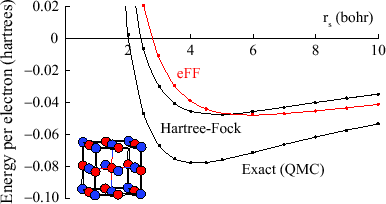
\includegraphics[scale=0.5]{corr}
\end{figure}
Questa energia di correlazione ha origine da $2$ diversi contributi:
\begin{itemize}
\item Correlazione tra elettroni con spin \emph{opposti} detta di Fermi. Può essere:
\begin{itemize}
\item Intra-orbitalica o \emph{dinamica};
\item Inter-orbitalica o \emph{statica};
\end{itemize}
\item Correlazione tra elettroni con spin \emph{paralleli} detta di Coulomb. Può essere:
\begin{itemize}
\item Intra-orbitalica o \emph{dinamica}: Tra elettroni dello stesso orbitale ($\sim 10^1-10^2 \quad KJ/mol$);
\item Inter-orbitalica o \emph{statica}: Tra elettroni di orbitali diversi ($\sim 10^0-10^1 \quad KJ/mol$ se tra orbitali non degeneri, altrimenti diventa comparabile con quella intra-orbitalica);
\end{itemize}
\end{itemize}
In termini di densità elettronica si possono visualizzare le differenze tra  correlazione \emph{statica e dinamica} \index{correlazione !statica }\index{correlazione !dinamica}  rispettivamente come: la \emph{repulsione} tra elettroni localizzati (statici) su orbitali differenti, e la repulsione tra elettroni che, occupando lo stesso orbitale, possono interagire istantaneamente (moto dinamico).
Il contributo principale deriva dalla correlazione di Coulomb (elettrostatica), quindi nella maggior parte dei metodi non viene presa in considerazione la correlazione di Fermi.
Risulta necessario elaborare dei metodi che descrivano questa energia di correlazione in quanto, variando con la geometria, non risulta possibile fare confronti tra geometrie di diversi step della stessa reazione.
\section{Determinanti di Slater di stati eccitati}
La logica dietro tutti i metodi post-HF sta nel descrivere la funzione d'onda multielettronica molecolare non più come un singolo determinante di Slater, ovvero come un generatore dello spazio di Hilbert, ma come una combinazione lineare dei generatori dello spazio della funzione d'onda, quindi far rientrare lo \emph{stato fondamentale} nella categoria degli \emph{stati quantistici misti}. Così facendo, lo stato fondamentale viene descritto da una combinazione lineare di stati ortogonali tra loro che definiscono lo spazio di esistenza della funzione d'onda.
\begin{equation}
\label{elio}
\Psi=\sum \limits _i ^{MaxEc} a_i \Phi_i
\end{equation}
 Una simile trattazione allarga spazialmente la funzione d'onda dello stato fondamentale  e, conseguentemente, riduce la probabilità che $2$ elettroni identici occupino lo stesso volume di spazio. Ciò permette di evitare gli errori dovuti alla \emph{correlazione dinamica}, tuttavia non riesce a descrivere a pieno il contributo della \emph{correlazione statica } che in sistemi \emph{diradicalici} risulta essere molto importante. Per descrivere tali sistemi sono stati sviluppati metodi più avanzati.
 La differenza principale tra i diversi metodi post-HF sta nell'algoritmo utilizzato per ottimizzare i coefficienti moltiplicativi della combinazione lineare riportata in Eq.\ref{elio}.
Il primo termine della combinazione lineare è sempre un determinante di Slater di tipo Hartree-Fock (RHF), mentre i termini successivi vengono generati a partire da questo determinante iniziale, andando a spostare gli elettroni da orbitali occupati a orbitali virtuali. Questi determinati dei termini successivi vengono associati a \emph{stati eccitati} e ogni spostamento di elettroni costituisce un'eccitazione:

\begin{figure}[H]
\centering
\caption{Visualizzazione dei diversi stati eccitati ai quali corrispondono diversi determinanti di Slater.}\label{E}
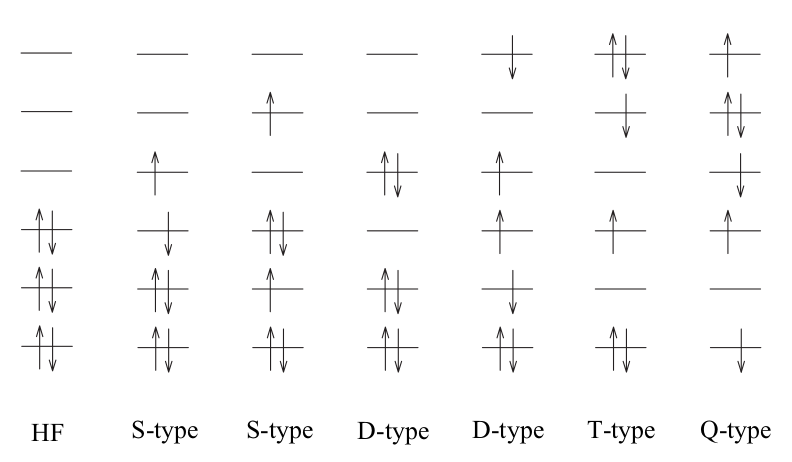
\includegraphics[scale=0.3]{exx}
\end{figure}

Ovviamente per ogni eccitazione  il numero di orbitali considerati dal calcolo aumenta fino al limite dettato dal set base, è infatti impossibile creare più orbitali di quante sono le combinazioni di orbitali atomici che rispettano i vincoli di simmetria dettati dalla geometria.
Immaginando quindi, di avere un set base infinito la funzione d'onda includerà tutte le possibili eccitazioni e l'equazione di Schr\"odinger sarà risolta esattamente entro i limiti dell'approssimazione di Born Oppenheimer non relativistica.
La qualità del calcolo dipenderà dunque dalla dimensione del set base e dalla quantità di eccitazioni considerate. Ciò rende applicabile un metodo "esatto" solo a molecole di pochi atomi, quindi praticamente inutile per la maggior parte dei sistemi reali. Per superare questo problema si possono attuare $2$ approssimazioni al metodo:
\begin{itemize}
\item \textbf{Frozen Core\index{Frozen Core}}: Dal momento che gli orbitali di interesse chimico sono solo quelli di valenza, si trascurano tutti gli elettroni di core. Ciò provoca un errore dal punto di vista dell'energia totale, dovuto alla correlazione dinamica degli elettroni di core. Tuttavia, dato che il loro contributo è praticamente costante, i risultati sono facilmente applicabili per valutare differenze. 
\item \textbf{Frozen Virtuals\index{Frozen Virtuals}}: Si escludono anche le combinazioni di antilegame che coinvolgono gli orbitali di core. Il costo del calcolo viene abbattuto sensibilmente.
\end{itemize}
Una volta ottenuta la combinazione lineare di determinanti di Slater ottimale per descrivere la funzione d'onda multielettronica si definiscono a partire da essa gli elementi della matrice hamiltoniana. Gli autovalori della matrice hamiltoniana così ottenuta corrisponderanno alle energie "esatte" dello stato fondamentale e di tutte le sue possibili eccitazioni.
Esistono $3$ metodi principali per trattare la \emph correlazione elettronica:
\begin{enumerate}
\item Interazione di configurazioni (CI)\index{CI}
\item Many-Body Perturbation Theory (MBPT)\index{MBPT}
\item Coupled Clusters (CC)\index{CC}
\end{enumerate}
Ognuno di questi metodi verrà trattato approfonditamente; bisogna però ricordare che per tutti questi metodi restano validi alcuni punti fissi:
\begin{enumerate}
\item L'operatore hamiltoniano è indipendente dallo spin che quindi viene preso come fattore moltiplicativo esterno alla matrice hamiltoniana;
\item Il determinante di HF è sempre di tipo RHF invece che del caso più generale di UHF;
\item Spesso nella risoluzione degli integrali ci sono doppie sommatorie con indici che corrono sulle stesse quantità. Questi indici saranno quindi sottoposti a limitazioni.
\end{enumerate}

\section{Interazione di configurazioni CI\index{CI}}
Questo metodo si basa sul principio variazionale per determinare i valori dei coefficienti della combinazione lineare di determinanti di Slater. Viene quindi imposta la condizione che l'energia della funzione d'onda multielettronica sia un minimo (si cerca un punto stazionario).
Gli orbitali molecolari monoelettronici utilizzati per costruire i determinanti di Slater sono quelli di Hartree-Fock e sono mantenuti fissi. Questo potrebbe portare a degli errori, infatti i sistemi dotati di una forte correlazione statica vengono descritti male da questi metodi. 
L'energia della funzione d'onda multielettronica deve essere quindi minimizzata tenendo conto della restrizione dovuta al fatto che $\Psi$ deve essere normalizzata.
Dovendo applicare questa restrizione la procedura d'eccellenza per minimizzare una funzione vincolata è il metodo di Lagrange. \index{Lagrange !metodo di}Definiamo ora la Lagrangiana di un simile sistema:

\begin{equation}
\begin{aligned}
\Psi_{CI}&= \sum \limits _i ^{m} a_i \Phi_i \\
\mathcal{L} &= \langle\Psi_{CI}\vert\hat{H}\vert\Psi_{CI}\rangle-\lambda\underbrace{(\langle\Psi_{CI}\vert\Psi_{CI}\rangle-1)}_{\text{Vincolo}}\\
\langle\Psi_{CI}\vert\hat{H}\vert\Psi_{CI}\rangle &= \sum \limits _i ^{m}\sum \limits _j ^{m} a_i a_j \langle\Phi_{i}\vert\hat{H}\vert\Phi_{j}\rangle =\sum \limits _i ^{m} a_i ^2 E_i + \sum \limits _i ^{m}\sum \limits _{i\neq j} ^{m}\langle\Phi_{i}\vert\hat{H}\vert\Phi_{j}\rangle \\
\langle\Psi_{CI}\vert\Psi_{CI}\rangle &= \sum \limits _i ^{m}\sum \limits _j ^{m} a_i a_j \langle\Phi_{i}\vert\Phi_{j}\rangle =  \sum \limits _i ^{m}a_i ^2
\end{aligned}
\end{equation}
Le sommatorie corrono fino al limite del set base in quanto esso definisce il massimo numero di eccitazioni che è possibile ottenere.
Una volta definita la \emph{lagrangiana} per cercarne i punti stazionari si pone la sua derivata rispetto i coefficienti $a_i$ uguale a $0$:
\begin{equation}
\begin{aligned}
\frac{\partial \mathcal{L}}{\partial a_i} = 2a_i E_i + \sum \limits_j a_j \langle\Phi_{i}\vert\hat{H}\vert\Phi_{j}\rangle -2\lambda a_i &=0\\
2 a_i (E_i - \lambda) + \sum \limits_{j\neq i}a_j \langle\Phi_{i}\vert\hat{H}\vert\Phi_{j}\rangle &= 0
\end{aligned}
\end{equation}
Quest'ultima equazione si può riscrivere in termini matriciali portando a destra l'energia,  ottenendo:
\begin{equation}
\hat{H}a=Ea
\end{equation}
Diagonalizzando la matrice dell'hamiltoniano CI si ottengono gli autovalori, quindi le energie, e gli autovettori quindi i coefficienti che moltiplicano i determinanti di Slater. Il più basso degli autovalori sarà l'energia dello stato fondamentale e il suo autovettore saranno i coefficienti della combinazione lineare che descrive lo stato fondamentale. Tutti gli altri autovalori saranno i vari stati eccitati.
\subsection{Elementi della matrice CI}
Per valutare gli elementi della matrice CI si adotta la stessa strategia usata per il metodo HF. Si espandono quindi i determinanti in termini di prodotto tra orbitali molecolari monoelettronici costruiti su funzioni atomiche del set base. Il problema principale è che l'hamiltoniano non include lo spin, quindi due determinanti uguali ma con spin diverso portano a una matrice a determinante nullo. Si costruiscono allora delle combinazioni lineari di determinanti che siano autovettori anche dell'operatore di spin dette \emph{Funzioni di configurazione di stato} (CSF). Queste funzioni sono a loro volta combinazioni lineari di determinanti di Slater che non sono autofunzioni dell'operatore di spin. Così facendo il numero di funzioni lievita facilmente in quanto ogni determinante di Slater viene generato per combinazione lineare di altri determinanti. Per ridurre la quantità di determinanti considerati si possono trascurare tutte le combinazioni lineari di autovettori ortogonali (nulle) e sfruttare la simmetria; inoltre dato che l'hamiltoniano è la \emph{somma di integrali mono e bielettronici} possiamo trascurare tutte le combinazioni lineari di orbitali che contengono elettroni più distanti spazialmente di 2 eccitazioni.
Definiamo quindi gli integrali monoelettronici come:
\begin{equation}
 \langle \Phi_{0}\vert \hat{H}\vert\Phi^{a}_i\rangle=\langle \phi_{i}\vert \hat{h}_i\vert\phi_{a}\rangle + \sum \limits _{j} \langle\phi_{i}\phi_j\vert g \vert\phi_{a}\phi_j\rangle-\langle\phi_{i}\phi_j\vert g \vert\phi_j\phi_{a}\rangle
\end{equation}
e gli integrali bielettronici come:
\begin{equation}
 \langle \Phi_{0}\vert \hat{H}\vert\Phi^{a}_i\rangle= \langle\phi_{i}\phi_j\vert g \vert\phi_{a}\phi_b\rangle-\langle\phi_{i}\phi_j\vert g \vert\phi_b \phi_{a}\rangle
\end{equation}
Conoscendo le espressioni per gli integrali mono e bielettronici possiamo definire gli elementi della matrice di Fock come: 
\begin{equation}
F_{ia}=\langle \phi_{i}\vert \hat{h}_i\vert\phi_{a}\rangle + \sum \limits _{j} \langle\phi_{i}\phi_j\vert g \vert\phi_{a}\phi_j\rangle-\langle\phi_{i}\phi_j\vert g \vert\phi_j\phi_{a}\rangle
\end{equation}
Da questa definizione della matrice di Fock possiamo capire che tale matrice sarà una diagonale a blocchi con sugli "assi" i determinanti di Slater. Risulta quindi evidente che se diagonalizzata si otterranno come elementi diagonali le energie delle diverse eccitazioni e come elementi extradiagonali le energie di interazione tra due stati eccitati o tra uno stato ecitato e quello fondamentale.
In merito all'energia di interazione tra uno stato eccitato e lo stato fondamentale bisogna citare il teorema di Brillouin:
\begin{equation}
\varepsilon_a \langle\phi_i\vert\phi_a\rangle = \varepsilon_a \delta_{ia}
\end{equation}
Ovvero singole eccitazioni che coinvolgono lo stato fondamentale (il determinante di HF)\emph{ hanno interazione nulla}, mentre gli elementi di matrice che afferiscono all'interazione tra una doppia eccitazione e il determinante HF avranno valori finiti. Per determinare gli elementi della matrice di Fock dobbiamo esprimere gli integrali mono- e bi-elettronici in termini del set base, quindi:
\begin{equation}
\begin{aligned}
\langle\phi_i\vert\hat{h}\vert\phi_a\rangle &= \sum\limits _{\alpha}^m \sum\limits _{\beta}^m c_{\alpha i} c_{\beta j} \langle\chi_{\alpha}\vert\hat{h}\vert\chi_{\beta}\rangle \\
\langle\phi_i\phi_j\vert\hat{h}\vert\phi_k\phi_l\rangle &= \sum\limits _{\alpha}^m \sum\limits _{\beta}^m \sum\limits _{\gamma}^m \sum\limits _{\delta}^m c_{\alpha i} c_{\beta j}c_{\gamma k} c_{\delta l}\langle	\chi_\alpha\chi_\beta\vert\hat{h}\vert\chi_\gamma\chi_\delta\rangle
\end{aligned}
\end{equation}
Dal momento che le $4$ sommatorie costituiscono ognuna il calcolo di un integrale, e tale calcolo deve essere svolto $m$ volte e successivamente ripetuto altrettante volte per $m$ eccitazioni si può dedurre che il metodo CI scali con $m^8$. Tuttavia esistono delle tecniche (trasformazioni a 4 indici) che permettono di ridurre questo costo computazionale a $m^5$. 
Dal momento che un simile costo computazionale è appena sostenibile da molecole di piccole dimensioni in quanto all'aumentare degli atomi aumenta il numero di eccitazioni da considerare con una legge fattoriale. Per rendere applicabile il metodo CI anche a molecole di medie dimensioni si applicano dei troncamenti al numero di eccitazioni considerate.
Così facendo il metodo resta \emph{variazionale} ma perde la sua \emph{size-consistency}.
\section{Size Consistency e Size Extensivity}
La \emph{size consistency} e la \emph{size extensivity} sono due concetti simili ma differenti. 
\begin{itemize}
\item \textbf{Size consistency}: Così è definita la capacità \emph{di un metodo} di descrivere sistemi composti da più molecole separate da distanze superiori ai $0.1 \quad nm$, quindi non interagenti. Per il CI troncato questa proprietà viene meno e si rischia di descrivere le eccitazioni di un sistema pluricomponente descrivendo anche determinanti misti tra le componenti del sistema;
\item \textbf{Size extensivity}: Così è definita la capacità di un metodo di descrivere frammenti lontani della stessa molecola come due zone non interagenti. Anche questa proprietà viene meno in un metodo CI troncato.
\end{itemize}
\section{Metodi Multi Configurational SCF MCSCF e CAS}
\subsection{MCSCF\index{MCSCF}}
Questa categoria di metodi include tutti quei metodi che cercano di superare la perdita in descrizione della \emph{correlazione statica} dovuta al fatto che solo i coefficienti della combinazione lineare di determinanti venissero ottimizzati, lasciando inalterati i coefficienti che definiscono i determinanti stessi. Se si ottimizzano anche i coefficienti dei determinanti all'interno di una combinazione lineare allora la funzione d'onda multielettronica si allargherà per effetto della combinazione lineare di determinanti ma, al contempo, gli orbitali molecolari monoelettronici si localizzeranno. Il risultato è che all'interno di una tipologia di eccitazione descritta da $n$ determinanti, gli orbitali che definiscono i singoli determinanti dell'eccitazione analizzata avranno energie diverse.
Le funzioni d'onda così generate sono più semplici da trattare di quelle di un CI ma non c'è la garanzia che il metodo converga a un minimo, quindi spesso si fa uso di una procedura SCF quadratica. La conseguenza principale sta in un aumento del costo computazionale. Un vantaggio di questi metodi sta nel fatto che le funzioni di stato configurazionale sono stati di spin puri quindi un metodo MCSCF non soffre gli effetti della contaminazione di spin.
Si possono quindi usare metodi di questo tipo per descrivere bene piccoli sistemi a molteplicità di spin elevata.
Il problema principale è l'elevatissimo costo computazionale che rende proibitivo l'uso di un MCSCF per sistemi già di medie dimensioni. Per superare questo problema sono stati sviluppati i metodi CAS.
\subsection{CAS\index{CAS}}
Nei metodi CAS si escludono alcuni orbitali dall'ottimizzazione dei coefficienti nei determinanti di Slater. Si dividono gli orbitali in due set:
\begin{itemize}
\item Spazio attivo: Insieme di orbitali che contribuiscono alla reattività della molecola (intorno a HOMO e LUMO).
\item Spazio inattivo: tutti gli orbitali che danno un contributo minoritario alla reattività della molecola (tipicamente gli orbitali di core e i virtuali più lontani dal LUMO).
\end{itemize}
Si indicano, quindi, quanti elettroni ($n$) sono distribuiti in quanti orbitali ($m$) con la notazione [n,m]-CASSCF.
Se il numero di orbitali considerato è elevato, con il metodo CAS si esegue un full CI su tutti gli orbitali dello spazio attivo, senza alcun guadagno di tempo. Sono stati quindi sviluppati metodi che dividono lo spazio attivo in zone, in ognuna delle quali lo sviluppo del full CI viene troncato a una specifica eccitazione (Fig.\ref{Ras}). Questi metodi prendono il nome di RAS.

\begin{figure}[H]
\centering
\caption{Diverse eccitazioni per diverse porzioni dello spazio attivo.}\label{Ras}
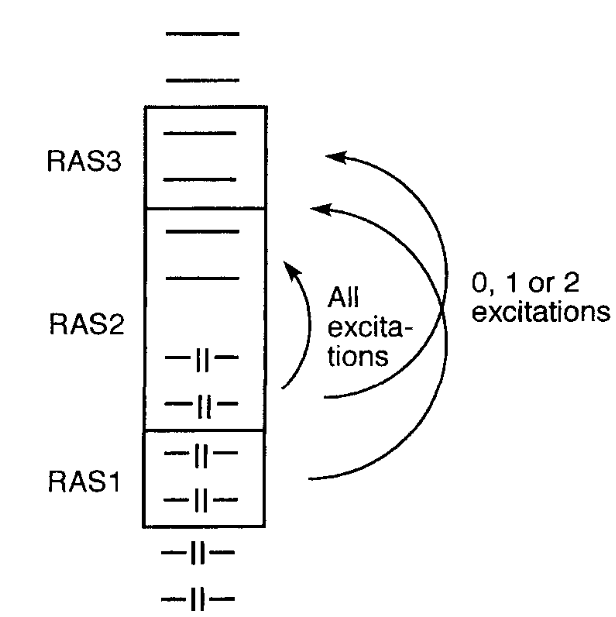
\includegraphics[scale=0.3]{ras}
\end{figure}

Una suddivisione dello spazio attivo come quella in figura \ref{Ras} permette un abbassamento del costo computazionale significativo.\\
La scelta dello spazio attivo può non essere sempre banale in quanto una diversa dimensione del CAS potrebbe considerare porzioni diverse dell'energia di correlazione. Diventa quindi cruciale mantenere alcune rgole di base per la scelta di un valido CAS:
\begin{enumerate}
\item Maggiore è il numero di orbitali di valenza inclusi maggiore è la precisione ma aumenta anche il costo computazionale.
\item Basarsi su un calcolo RHF per capire l'ordine degli orbitali è una buona strategia nella maggior parte dei casi. Tuttavia se i livelli degli orbitali virtuali sono troppo vicini si può incorrere in errori gravi.
\item Conviene includere orbitali con occupazioni ben precise (0 o 2).
\end{enumerate}
I metodi MCSCF possono essere utilizzati anche per generare una funzione d'onda di stato fondamentale da utilizzare come riferimento in metodi diversi come in un CI. Ciò presenta l'ovvio vantaggio di lavorare con una funzione d'onda già ottimizzata, ma ovviamente aumenta le tempistiche dei calcoli. Metodi CI che implementano questa possibilità si chiamano MRCI (Multi reference CI).
\section{Metodi Many-Body Perturbation Theory MBPT\index{MBPT}}
In questi metodi l'idea guida è che il sistema analizzato differisca di poco da un sistema ideale già calcolato in precedenza.
Di conseguenza si costruisce un hamiltoniano come somma del sistema di riferimento e di una perturbazione che corregga le piccole differenze tra i sistemi.
\begin{equation}
H=H_0+\lambda H'
\end{equation}
Il termine perturbativo viene pesato per un coefficiente $\lambda$ che indica l'entità della perturbazione.
Tipicamente il sistema di riferimento genera un hamiltoniano con l'approssimazione delle particelle indipendenti, mentre la perturbazione corregge questa approssimazione introducendo l'interazione tra particelle. I metodi che utilizzano questa descrizione dell'hamiltoniana si chiamano MBPT.
\subsection{L'energia nei metodi MBPT}
Dato che l'entità della perturbazione viene aumentata progressivamente, anche la funzione d'onda e l'energia subiranno progressive variazioni, descrivibile come sviluppo in serie.
\begin{equation}
\begin{aligned}
H\Psi &=  W \Psi \\
W &= \sum \limits _{i=0} ^n \lambda^i W_i \\
\Psi &= \sum \limits _{i=0} ^n \lambda^i \Psi_i 
\end{aligned}
\end{equation}
Per $\lambda = 0, \quad H= H_0$ allora vale $\Psi_0 = \Phi_0 $ e $W_0=E_0$ ovvero si ha la perturbazione di ordine 0 che corrisponde al sistema imperturbato. Scegliendo un opportuno valore di $n$ si stabilisce l'ordine al quale troncare la perturbazione, e l'hamiltoniano che ne risulta conterrà tutti i termini fino alla perturbazione scelta.
Per quanto riguarda la funzione d'onda, è opportuno scegliere una funzione d'onda perturbata $\Psi$ che dia overlap perfetto con la funzione imperturbata e che sia quindi ortogonale a tutti i vari ordini di perturbazione.
\begin{equation}
\begin{aligned}
\langle\Psi\vert\Phi_0\rangle &= 1 \\
\langle  \sum \limits _{i=0} ^n \lambda^i \Psi_i \vert \Phi_0 \rangle &= 1 \\
\underbrace{\langle\Phi_0\vert\Phi_0\rangle}_{=1} + \underbrace{\lambda\langle\Psi_1\vert\Phi_0\rangle + \lambda^2\langle\Psi_2\vert\Phi_0\rangle + \ldots}_{=0} &= 1
\end{aligned}
\end{equation}
Quindi possiamo riscrivere l'equazione di Scr\"odinger come:
\begin{equation}
(H_0+\lambda H')( \sum \limits _{i=0} ^n \lambda^i \Psi_i)=(\sum \limits _{i=0} ^n \lambda^i W_i)( \sum \limits _{i=0} ^n \lambda^i \Psi_i)
\end{equation}
Possiamo ora raccogliere i termini moltiplicati per i diversi valori di $\lambda$
\begin{equation}
\label{MBPorcodio}
\begin{aligned}
&\lambda^0 : H_0 \Psi_0 = W_0 \Psi_0 \\
&\lambda^1 : H_0 \Psi_1 + H'\Psi_0 = W_0 \Psi_1 + W_1 \Psi_0\\
&\lambda^2 : H_0 \Psi_2 + H'\Psi_1 = W_0 \Psi_2 + W_1 \Psi_1 + W_2 \Psi_0 \\
&\lambda^n : H_0 \Psi_n + H'\Psi_{n-1} = \sum \limits _{i=0} ^n W_i \Psi_{n-i}
\end{aligned}
\end{equation}
A parte il primo termine che è l'equazione di Schr\"odinger nel caso imperturbato, tutti gli altri termini contengono i termini incogniti di hamiltoniano, energia e funzione d'onda corretti al n-esimo ordine. Tali incognite possono essere ricavate applicando la regola del turnover:

\begin{equation}
\begin{aligned}
\langle \Phi_0 \vert H_0 \vert \Psi_n\rangle + \langle \Phi_0 \vert H' \vert \Psi_{n-1} \rangle = \underbrace{\sum \limits _{i=0} ^{n-1} W_i \langle \Phi_0 \vert \Psi_0 \rangle}_{=0 \text{ per } n\geq 2} \\
\text{Ricordando che: } H_0\vert \Phi_0 \rangle = E_0 \vert \Phi_0 \rangle \\
E_0\underbrace{\langle \Psi_n \vert \Phi_0\rangle}_{=0} + \langle \Phi_0 \vert H' \vert \Psi_{n-1} \rangle =  W_n \underbrace{\langle \Phi_0 \vert \Psi_0 \rangle}_{=1} \\ \\
W_n= \langle \Phi_0 \vert H' \vert \Psi_{n-1}\rangle
\end{aligned}
\end{equation}
Da questa equazione possiamo intuire che al fine di valutare l'energia al n-esimo ordine sia necessario conoscere almeno la funzione d'onda all'ordine $n-1$. In realtà conoscere una funzione d'onda all'ordine $n$ ci permette di conoscere l'energia all'ordine $2n+1$:
\begin{equation}
W_{2n+1} = \langle \Psi	_n \vert H'\vert \Psi_n \rangle - \sum \limits _{k,l=0} ^n W_{2n+1-k-l} \langle \Psi_k \vert \Psi_l \rangle
\end{equation}
Nonostante gli sforzi fatti alcune quantità restano incognite, in particolare l'energia e la funzione d'onda. Tuttavia se troviamo un modo di esprimere la funzione d'onda in termini di qualcosa di conosciuto come i determinanti delle eccitazioni di Hartree Fock.
\begin{equation}
\label{kak?}
\Psi_1= \sum_i a_i \Phi_i
\end{equation}
Espandendo in questo modo la funzione d'onda perturbata al primo ordine possiamo inserire una tale definizione nel raccoglimento di $\lambda^1$ fatto in Eq.\ref{MBPorcodio} ottenendo:

\begin{equation}
\begin{aligned}
\sum_i a_i\langle \Phi_0 \vert H_0 \vert \Phi_i \rangle - \underbrace{W_0 \sum_i a_i \langle \Phi_0 \vert \Phi_i \rangle}_{= a_0E_0} +\langle \Phi_0 \vert H' \vert \Phi_0  \rangle -W_1\underbrace{ \langle \Phi_0\vert \Phi_0\rangle}_{=1} &= 0\\
\sum_i a_i E_i \langle \Phi_0\vert \Phi_i \rangle -a_0 E_0 + \langle \Phi_0 \vert H' \vert \Phi_0 \rangle - W_1 &= 0 \\
a_0 E_0 -a_0E_0 + \langle \Phi_0 \vert H' \vert \Phi_0 \rangle - W_1 &= 0 \\ \\
W_1 = \langle \Phi_0 \vert H' \vert \Phi_0 \rangle
\end{aligned}
\end{equation}

In questa equazione $W_1$ rappresennon esisteta l'energia media dovuta alla perturbazione del primo ordine sulla funzione d'onda imperturbata.
Restano quindi da definire i valori dei coefficienti che entrano nella combinazione lineare di equazione \ref{kak?} così da eliminare tutti i fattori incogniti. Ciò è ricavabile mediante il procedimento in Eq. \ref{kak chto?}.

\begin{equation}
\label{kak chto?}
\begin{aligned}
\sum_i a_i\langle \Phi_j \vert H_0 \vert \Phi_i \rangle - \underbrace{W_0 \sum_i a_i \langle \Phi_j \vert \Phi_i \rangle}_{= a_jE_j\text{ se }j=i} +\langle \Phi_j\vert H' \vert \Phi_0  \rangle -W_1\underbrace{ \langle \Phi_j\vert \Phi_0\rangle}_{=0} &= 0\\
\sum_i a_i E_i \langle \Phi_j\vert \Phi_i \rangle -a_0 E_0 + \langle \Phi_j \vert H' \vert \Phi_0 \rangle  &= 0 \\
a_j E_j -a_jE_0 + \langle \Phi_j \vert H' \vert \Phi_0 \rangle  &= 0 \\ \\
a_j = \frac{\langle \Phi_j \vert H' \vert \Phi_0 \rangle}{E_0-E_j}
\end{aligned}
\end{equation}

Questi coefficienti prendono il nome di \emph{coefficienti di espansione} e definiscono la funzione d'onda perturbata al primo ordine. Si possono ricavare con un processo analogo le energie e i coefficienti per tutti gli ordini successivi. Il risultato di una simile operazione produce gli elementi di una matrice che descrive l'operatore \emph{perturbazione}, che applicato e diagonalizzato genera le funzioni perturbate e le energie associate.  
  non aggiunge voci
\subsection{La teoria di M{\o}ller- Plesset\index{M{\o}ller- Plesset}}
Questa teoria è necessaria per definire una forma dell'\emph{hamiltoniano perturbato}, ovvero l'ultimo elemento incognito necessario per trovare l'energie associate alle perturbazioni e i coefficienti ai determinanti di Slater.
Secondo questa teoria l'hamiltoniano imperturbato viene costruito come sommatoria di operatori di Fock:
\begin{equation}
\begin{aligned}
H_0 &= \sum \limits _{i=0} ^{N_e} F_i \\
&= \sum \limits _{i=0} ^{N_e} \left( h_i +\sum \limits _{j=0} ^{N_e} (J_j-K_j)\right) \\
&= \sum \limits _{i=0} ^{N_e} h_i + \sum \limits _{i=0} ^{N_e}\sum \limits _{j=0} ^{N_e} \langle g_{ij} \rangle \\
&g_{ij} \text{ rappresenta il potenziale medio di interazione tra 2 elettroni: } V_{ee}\\
&= \sum \limits _{i=0} ^{N_e} h_i +  \langle V_{ee} \rangle \\
&\text{Ricordando che l'hamiltoniano corretto è:}\\
H &= \sum \limits _{i=0} ^{N_e} h_i + V_{ee} \\
&\text{Possiamo sottrarre l'hamiltoniano imperturbato a quello corretto} \\
 &\text{per ricavare il valore della perturbazione:}\\
H' &= H- H_0 = V_{ee}-2  \langle V_{ee} \rangle
\end{aligned}
\end{equation}
Da questa equazione risulta evidente che la somma degli operatori di Fock conta il doppio dell'interazione interelettronica. Infatti l'energia all'ordine 0 è data dalla somma delle energie dei singoli orbitali:
\begin{equation}
W_0= \sum \limits _{i=0} ^{N_e} \varepsilon_i
\end{equation}
Tuttavia queste energie derivano dal considerare l'elettrone che percepisce la repulsione media di tutti gli altri elettroni. Quindi sommando tali energie ogni elettrone percepirà un campo medio generato dal doppio degli elettroni realmente presenti.
Includendo il contributo della prima perturbazione questo conteggio doppio viene eliminato:
\begin{equation}
W_1 =  \langle V_{ee} \rangle-2  \langle V_{ee} \rangle = -\langle V_{ee} \rangle
\end{equation}
Quindi introducendo il primo termine perturbativo si corregge la somma delle energie degli orbitali e si ottiene esattamente l'energia di \emph{Hartree-Fock}.
Si deduce quindi che i primi termini che daranno un contributo in termini di energia di correlazione saranno quelli al secondo ordine.
\begin{equation}
W_2= \frac{\langle \Phi_0 \vert H' \vert \Phi_i \rangle \langle \Phi_i \vert H' \vert \Phi_0 \rangle}{E_0-E_i}
\end{equation}
Considerando i vari determinanti associati alle varie eccitazioni, ci si rende conto che la prima eccitazione non influenza l'energia a causa del teorema di Brillouin:
\begin{equation}
\langle \Phi_0 \vert H' \vert \Phi_i \rangle = \underbrace{\langle \Phi_0 \vert H \vert \Phi_i \rangle}_{=0 \text{ per Brillouin}} - \sum \limits _{i=0} ^{N_e} \varepsilon_i \underbrace{\langle \Phi_0\vert\Phi_i\rangle}_{=0}=0
\end{equation}
Quindi l'energia associata al secondo ordine di perturbazione è generata esclusivamente da integrali bielettronici e si può esprimere come:
\begin{equation}
W_2=\sum \limits _{i<j} ^{occ}\sum \limits _{a<b} ^{virt} \frac{\vert\langle \phi_i \phi_j \vert g_{ij} \vert \phi_a \phi_b \rangle- \langle  \phi_i \phi_j\vert g_{ij} \vert \phi_a \phi_b \rangle \vert ^2}{\varepsilon_i+\varepsilon_j-\varepsilon_a-\varepsilon_b}
\end{equation}
Con questo metodo si riesce a descrivere fino all $80-90 \%$ della correlazione elettronica a fronte di un costo computazionale relativamente basso, circa uguale a quello del HF.
Il problema principale è dovuto al fatto che l'uso di questo metodo somma l'errore dovuto alla finitezza del set base all'errore dovuto al troncamento dello sviluppo della perturbazione. Questi errori sono particolarmente visibili se la geometri del sistema è lontana dall'equilibrio o se si sta cercando di descrivere stati eccitati.
Il metodo troncato al secondo ordine prende il nome di MP2. Sulla base di questo metodo sono stati sviluppati metodi analoghi che considerano separatamente le componenti statica (spin-orbitale) e dinamica (spin-spin) dell'energia di correlazione. Tali metodi presentano un'efficienza computazionale superiore e talvolta scalano meglio di un HF.\\
Troncando a ordini superiori la perturbazione si ottengono i metodi successivi ovvero MP3, MP4, MP5, ... Tuttavia l'ultimo che garantisce un'applicabilità su grande scala è il MP4 che riesce a descrivere fino al $98\%$ dell'energia di correlazione.
Tutti questi metodi sono \emph{size consistent}\index{size consistency} ma non sono variazionali, pertanto possono produrre energie anche inferiori rispetto a quella reale. L'errore che commettono resta però costante grazie alla size consistency e ciò permette di utilizzarli per effettuare calcoli di differenze di energia.
Il principale limite di questi metodi è dovuto alla stima della funzione d'onda iniziale, in quanto non sempre una funzione d'onda di Hartree-Fock rientra nell'assunzione che la $\Psi_0$ di riferimento debba essere molto simile a quella reale. 
\section{Metodi Coupled Clusters CC \index{CC}}
Mentre nei metodi perturbativi si troncano tutti i tipi di correzione a un determinato ordine, nei metodi \emph{coupled cluster} si includono tutte le correzioni di un determinato tipo sviluppate a ordine infinito.
Per fare ciò è necessario definire un operatore eccitazione che  se applicato a una funzione d'onda di riferimento ne genera tutte le possibili eccitazioni di un certo tipo (S, D, T, Q,...).
\begin{equation}
\Psi_{CC}=e^{T}\Phi_0
\end{equation}
Con:
\begin{equation}
T= T_1+T_2+T_3+T_4+T_5+T_6+T_7+T_8+\ldots
\end{equation}
Ogni possibile eccitazione  è quindi inclusa in un operatore ($e^{T}$) che se espanso in serie di Taylor\index{serie di !Taylor} permette di raccogliere i termini delle singole eccitazioni:
\begin{equation}
e^T=1+T_1+(T_2+\frac{1}{2}T_1^2)+(T_3+T_2T_1+\frac{1}{6}T_1^3)+\ldots
\end{equation}
Per ogni eccitazione sono inclusi dei termini aggiuntivi detti \emph{connessi} dati dai prodotti tra eccitazioni pure e fisicamente sono visualizzabili come le interazioni tra coppie di elettroni mentre i termini \emph{disconnessi} dovuti all'eccitazione diretta sono ascrivibili all'interazione tra singoli elettroni. 
Possiamo quindi ora riscrivere l'equazione di Schr\"odinger per il caso CC:
\begin{equation}
H e^T \Phi_0= E_{CC} e^T\Phi_0
\end{equation}
Impostando la definizione dell'energia sulla base del \emph{teorema variazionale} si ottiene:
\begin{equation}
E^{var}_{CC}= \frac{\langle e^T\Phi_0 \vert H \vert e^T\Phi_0 \rangle }{\langle e^T\Phi_0\vert e^T\Phi_0 \rangle}
\end{equation}
Sviluppando l'esponenziale fino all'ultimo termine ($N_e$) si ottiene un equazione ricca di un gran numero di termini che se calcolati renderebbero il metodo applicabile solo a piccole molecole. Tuttavia tali termini includendo i contributi delle varie eccitazioni \emph{non possono essere trascurati}. La soluzione per rendere il metodo un po' più flessibile sta nel \emph{proiettare l'equazione di Schr\"odinger CC } sulla funzione d'onda di riferimento:
\begin{equation}
\begin{aligned}
\langle \Phi_0 \vert H e^T\vert \Phi_0 \rangle &= E_{CC}\langle \Phi_0 \vert e^T\Phi_0 \rangle\\
\langle \Phi_0 \vert H e^T\vert \Phi_0 \rangle &= E_{CC}\langle \Phi_0 \vert (1+T_1+T_2+T_3+\ldots)\Phi_0 \rangle\\
&\text{Ricordando che vengono generati determinanti di Slater eccitati:} \\
\delta_{0i} &= \langle \Phi_0 \vert (1+T_1+T_2+T_3+\ldots+T_i)\Phi_0 \rangle\\
&\text{Quindi:}\\ \\
E_{CC}&=\langle \Phi_0 \vert H e^T\vert \Phi_0 \rangle 
\end{aligned}
\end{equation}
Possiamo ora espandere l'operatore eccitazione in serie di Taylor:
\begin{equation}
\begin{aligned}
E_{CC}&=\langle \Phi_0 \vert H e^T\vert \Phi_0 \rangle  \\
&= \underbrace{\langle \Phi_0 \vert H \vert \Phi_0 \rangle}_{E_0}+\underbrace{\langle \Phi_0 \vert H \vert T_1\Phi_0 \rangle}_{=0}+\langle \Phi_0 \vert H \vert T_2 \Phi_0 \rangle+ \frac{1}{2} \langle \Phi_0 \vert H \vert T_1^2 \Phi_0 \rangle\\
&= E_0+ \sum \limits _{i<j} ^{occ}\sum \limits _{a<b} ^{virt}\left(t_{ij}^{ab}+t^a_it^b_j+t^b_it^a_j\right)\langle\Phi_0\vert H\vert\Phi^{ab}_{ij}\rangle \\
&= E_0+ \sum \limits _{i<j} ^{occ}\sum \limits _{a<b} ^{virt}\left(t_{ij}^{ab}+t^a_it^b_j+t^b_it^a_j\right) \left(\langle \phi_i \phi_j \vert g_{ij} \vert \phi_a \phi_b \rangle- \langle  \phi_i \phi_j\vert g_{ij} \vert \phi_a \phi_b \rangle\right)
\end{aligned}
\end{equation}
I coefficieti $t$ sono detti ampiezze e determinano il tipo di eccitazione applicato. Essi sono degli scalari in quanto descrivono, in questo caso, il peso degli integrali mono e bielettronici in ogni singola eccitazione.
Considerare tutte le possibili eccitazioni sviluppate al massimo ordine produce risultati analoghi a quelli di un Full CI, ma i tempi di un calcolo simile risultano essere proibitivi anche per molecole di medie dimensioni. Per ampliare il range di applicabilità di questa categoria di metodi sono stati svilluppati i metodi CC \emph{troncati}.
Nei metodi CC troncati l'operatore eccitazione viene troncato a un preciso termine e si considerano solo le eccitazioni fino al termine di troncamento:
\begin{enumerate}
\item Singole: $T=T_1$ CCS;
\item Doppie: $ T= T_2$ CCD;
\item Sigole e doppie: $T= T_1+T_2$ CCSD;
\item ecc. ecc.
\end{enumerate}
Per aumentare l'accuratezza di questi metodi troncati senza inficiarne ulteriormente l'efficienza computazionale sono stati derivati dei metodi ibridi con quelli basati sulla teoria di M{\o}ller-Plesset. Questi metodi ibridi calcolano i contributi delle eccitazioni superiori con la formula derivante dal MP4 ma invece di derivarsi i coefficienti della funzione d'onda vengono utilizzate le ampiezze del metodo CC immediatamente precedente. Portiamo a esempio il caso del CCSD(T) in cui i contributi delle triple eccitazioni derivano da un conto MP4 che sostituisce i coefficenti con le ampiezze calcolate al livello CCSD. 

\section{Metodi Quantum Monte-Carlo QMC}
Con metodi \emph{Monte Carlo}\index{Monte Carlo} si intendono tutti quei metodi che stimano il valore di un integrale multidimensionale di una funzione valutandone il valore casualmente nello spazio delle variabili e calcolando il valore dell'integrale finale come media statistica delle stime casuali. Nel limite di un campionamento casuale infinito il valore calcolato coincide con quello reale, ma se il campionamento è finito si dovrà riportare il risultato accompagnato dalla sua \emph{deviazione standard}.
Si possono applicare tali metodi ai problemi della meccanica quantistica perché il quadrato della funzione d'onda è una probabilità, quindi integrabile con un metodo \emph{Monte Carlo}.
\begin{equation}
\begin{aligned}
E&=\frac{\langle\Phi\vert H\vert \Phi \rangle}{\langle\Phi\vert\Phi\rangle} \\
&= \frac{\int \Phi^* \Phi (\Phi^{-1}H\Phi) dr}{\int \Phi^*\Phi dr} \\
&= \frac{\int\vert \Phi\vert^2 (\Phi^{-1}H\Phi) dr}{\int \vert \Phi\vert^2 dr} 
\end{aligned}
\end{equation}
Definiamo ora:
\begin{equation}
\begin{aligned}
E_{locale} &= \Phi^{-1}H\Phi \\
P(r) &=\frac{\vert \Phi\vert^2 }{\int \vert \Phi\vert^2 dr} 
\end{aligned}
\end{equation}
Quindi:
\begin{equation}
\begin{aligned}
E= \int E_{locale} P(r) dr
\end{aligned}
\end{equation}
Ovvero l'energia totale di un sistema è data dall'integrale dell'energia valutata localmente pesata per la probabilità che l'elettrone si trovi in quel volume di spazio.
Questo integrale può essere valutato con metodi Monte Carlo se si conosce la forma funzionale della funzione d'onda che definisce $P(r)$. Una volta ricavata la probabilità i punti di campionamento vengono generati su questa distribuzione mediante l'algoritmo \emph{Metropolis}. Le funzioni d'onda utilizzate per generare la distribuzione di probabilità sono solitamente delle funzioni d'onda HF \emph{moltiplicate per una correzione dovuta alla correlazione}. Questa correzione prende forma nella funzione di \emph{Jastrow}.
Questi metodi scalano tipicamente con un paio di ordini di grandezza in più rispetto HF e DFT rendendoli competitivi solo con i CC e i CI. Il più grande limite di questi metodi è dovuto all'intrinseco errore statistico che accompagna ogni risultato e che rende difficile calcolare vettori forza per le ottimizzazioni, e derivate seconde per le frequenze.





\chapter{Set di funzioni base}
Nei metodi \emph{ab initio} si cerca di derivare tute le informazioni relative a un sistema reale senza coinvolgere dati sperimentali. Per fare ciò è necessario, come già visto nei capitoli precedenti, definire un operatore hamiltoniano che se applicato alla funzione d'onda, definita come determinante di Slater, restituisce l'energia del sistema. Fin'ora i nostri sforzi si sono concentrati su due dei tre ingredienti che costituiscono l'equazione di Schr\"odinger, ovvero l'hamiltoniano e l'energia. Tuttavia abbiamo già visto che anche la funzione d'onda deve essere approssimata. Una tale approssimazione della funzione d'onda deriva, come già visto, dal metodo LCAO\index{LCAO}. Possiamo quindi ripercorrere a ritroso tutti i passaggi che ci portano a costituire la funzione d'onda multielettronica molecolare sino a giungere alle funzioni di base, ovvero la seconda informazione di un input di un qualsiasi programma di calcoli quantomeccanici \emph{ab initio}.
\begin{equation}
\Psi\Longrightarrow\Phi\Longrightarrow\phi\Longrightarrow\chi
\end{equation} 
In questa scala gerarchica abbiamo:
\begin{enumerate}
\item $\Psi$: Funzione d'onda molecolare multielettronica reale che ci interessa descrivere;
\item $\Phi$: Determinante di Slater che fornisce un'approssimazione abbastanza puntuale della funzione d'onda reale;
\item $\phi$: Funzioni molecolari \emph{monoelettroniche} chiamate \emph{spin-orbitali}. Essendo delle distribuzioni di probabilità di elettroni singoli il loro prodotto, in forma di determinante di Slater, descrive la distribuzione multielettronica;
\item $\chi$: Funzioni atomiche che se combinate linearmente costituiscono gli orbitali, ai quali viene moltiplicata una funzione atta a descrivere la coordinata di spin. La definizione funzionale di queste funzioni e quante di esse siano necessarie per dare una descrizione fisicamente coerente del sistema, sono gli argomenti di questo capitolo. 
\end{enumerate}
Come appena accennato la parte orbitalica degli spin-orbitali secondo l'approssimazione LCAO deve essere descritta da una combinazione lineare di orbitali atomici, i quali saranno descritti dalle funzioni base\index{funzioni base} $\chi$:
\begin{equation}
\phi_i(r,\sigma)= \phi_i(r)\sigma (i) \quad \rightarrow \quad \phi_i(r)= \sum \limits _{\mu} ^m c_{i,\mu} \chi_\mu (r,R)
\end{equation}
Le funzioni di base avranno una dipendenza intrinseca dalle coordinate elettroniche ma dovranno essere localizzate in prossimità degli atomi, dipendendo, quindi, anche dalle coordinate nucleari. Tuttavia nel caso reale ogni atomo possiede più funzioni atomiche, pertanto anche i set base dovranno contenere diverse funzioni base per ogni atomo. Il caso ideale è quello di uno sviluppo infinito del set base (set base completo), che genererebbe la funzione d'onda esatta. Ciò è impossibile se si lavora con un calcolatore, che per sua natura è limitato, pertanto è necessario scegliere una dimensione massima del set base\index{set base}. A seconda della dimensione $m$ scelta si otterranno risultati con accuratezze differenti.
Dobbiamo ora definire una serie di caratteristiche che le funzioni base devono possedere affinché portino a dei risultati dell'accuratezza desiderata:
\begin{enumerate}
\item La forma funzionale deve riflettere la natura del problema in modo da poter usare un minor numero di funzioni base, ma al contempo deve essere facilmente integrabile;
\item Le funzioni base dovrebbero poter generare un set base completo, in modo da poterlo troncare a un limite ben definito;
\item I set base dovrebbero essere disponibili a differenti livelli gerarchici in modo che al massimo livello della gerarchia  convergano al limite del set base;
\item A un certo livello di accuratezza il set base deve essere computazionalmente efficiente, quindi usare il minor numero di funzioni base possibile;
\item I set base dovrebbero essere universali e applicabili, quindi, con qualsiasi metodo per qualunque proprietà. Questo principio sottintende che si debbano utilizzare molte funzioni base, vìolando il punto precedente;
\item Deve essere disponibile almeno un set base per ogni atomo della tavola periodica.
\end{enumerate}
La qualità complessiva di un set base è quindi data dal compromesso tra \emph{universalità} ed \emph{efficienza}. Andiamo ora a indagare quali forme funzionali siano state selezionate negli anni come migliori candidate alla descrizione delle funzioni di base.
\section{Tipi di funzioni base}
Esistono $2$ tipi di funzioni che vengono tipicamente utilizzate nella descrizione degli orbitali atomici:
\begin{itemize}
\item \emph{Slater Type Orbitals STO};
\item \emph{Gaussian Type Orbitals GTO}.
\end{itemize}
\subsection{STO \index{STO}}
Le funzioni atomiche di tipo Slater presentano la seguente forma funzionale:
\begin{equation}
\chi_{\zeta, n, l, m}(r, \vartheta, \varphi)= N Y_{l,m}(\vartheta, \varphi) r^{n-1} e^{-\zeta r}
\end{equation}
Dove:
\begin{enumerate}
\item $N$: è un fattore di \emph{normalizzazione};
\item $Y_{l,m}(\vartheta, \varphi)$: sono funzioni \emph{armoniche sferiche}, soluzioni dell'equazione di Schr\"odinger per l'atomo di idrogeno. Esse dipendono dal numero quantico secondario dando la forma all'orbitale, e dal numero quantico di momento orbitalico dando l'orientazione dell'orbitale;
\item $e^{-\zeta r}$: la dipendenza esponenziale dalla distanza elettrone-nucleo fa sì che questo tipo di funzioni non abbiano nodi nella parte radiale. Questo è irrealistico ma i nodi si possono ottenere facilmente mediante combinazioni lineari di STO.
\end{enumerate}
Dato che queste funzioni sono quelle fisicamente corrette, in quanto costruite sulla base della soluzione analitica dell'atomo di idrogeno, esse vanno a \emph{convergenza molto velocemente} ma a causa della difficoltà nel valutarne gli integrali non è possibile ottenere soluzioni analitiche per sistemi con più di 3/4 atomi. 
Questo tipo di funzioni trovano, quindi, applicazione in sistemi mono e biatomici o per metodi semiempirici che trascurano gli integrali a 3 e 4 centri, o ancora per metodi DFT\index{DFT} poiché non includono lo scambio esatto e i potenziali di Coulomb sono calcolati per fitting sulla densità elettronica.

\subsection{GTO\index{GTO}}
La forma funzionale di questo tipo di funzioni coincide con la definizione di gaussiana:
\begin{equation}
\chi_{\zeta,l_x,l_y,l_z}(x,y,z)= N x^{l_x}y^{l_y}z^{l_z}e^{-\zeta r^2}
\end{equation}
Tuttavia per comodità si preferisce esprimerla in un sistema polare per rispettare la simmetria sferica degli orbitali e utilizzare quindi un grado di libertà in meno:
\begin{equation}
\chi_{\zeta,n,l,m}(r, \vartheta, \varphi)= N Y_{l,m}(\vartheta, \varphi) r^{2n-2-l}e^{-\zeta r^2}
\end{equation}

L'utilizzo di funzioni gaussiane presenta sia vantaggi che svantaggi:
\begin{enumerate}
\item Il prodotto di due funzioni gaussiane è ancora una gaussiana. Quindi vale che:
$$\chi_\mu\chi_\lambda=\chi_\nu$$ e quindi gli integrali a quattro centri diventano integrali a due centri semplificandosi:
$$\langle\chi_\mu\chi_\lambda\vert g_{ij}\vert\chi_\mu\chi_\lambda\rangle=\langle\chi_\nu\vert g_{ij}\vert\chi_\nu\rangle$$
\item L'integrale di una funzione gaussiana è ancora una gaussiana e può essere svolto analiticamente a basso costo computazionale;
\item Le gaussiane non sono fisicamente accettabili in quanto:
\begin{itemize}
\item Sul nucleo non presentano un punto di cuspide come le STO;
\item La gaussiana decade troppo velocemente con la distanza.
\end{itemize}
\end{enumerate}
Questo singolo svantaggio implica che per ottenere un adeguato livello di accuratezza siano necessarie molte più GTO rispetto a quante STO si utilizzino solitamente. Tuttavia la facilità di calcolo degli integrali e l'efficienza computazionale delle GTO compensano sufficientemente l'ampia varietà di gaussiane da includere.
Inoltre si possono usare delle gaussiane a coefficienti fissi per costruire mediante combinazione lineare degli orbitali di tipo Slater aumentando così sia l'efficienza computazionale che la coerenza fisica.

\begin{figure}[H]
\centering
\caption{Combinazione lineare di gaussiane che approssima un orbitale STO.}\label{sto}
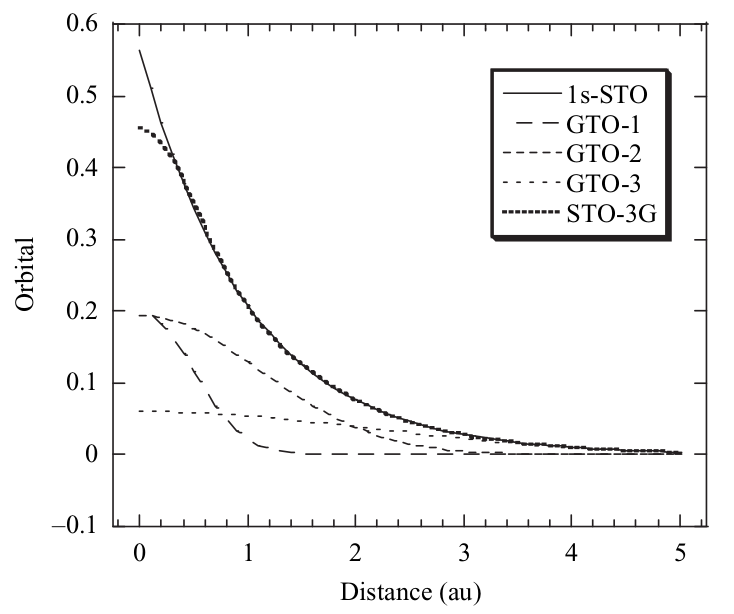
\includegraphics[scale=0.3]{sto}
\end{figure}


\section{Sdoppiamento dei set base e numero di Z}
Dopo aver definito le forme funzionali che caratterizzano le funzioni base, come già anticipato, è fondamentale capire in quale quantità queste funzioni vadano usate affinché sia garantito un certo grado di accuratezza.
Se pensiamo alle configurazioni elettroniche degli atomi che abbiamo imparato a fare durante i corsi del primo anno, viene intuitivo costruire il set base di ogni atomo con esattamente le funzioni della sua configurazione elettronica. Quindi:
\begin{itemize}
\item H e He: 1 funzione s;
\item 2° periodo: 2 funzioni s e 3 funzioni p;
\item 3° periodo: 3 funzioni s, 3 funzioni p;
\item ecc. ecc.
\end{itemize}
Se costruiamo il set base in questo modo, otterremo quello che viene definito set base \emph{minimo} o \emph{a singola Zeta} (facendo riferimento all'esponente della gaussiana). Sebbene un set base minimo sia sufficiente a risolvere gli esercizi di chimica generale, non lo è per eseguire calcoli di meccanica quantistica. Immaginiamo di dover descrivere un triplo legame: esso sarà costituito da una parte $\sigma$ localizzata tra i due atomi di un legame molto corto, quale è quello triplo, e da  due parti $\pi$ delocalizzate lontano dai nuclei e ortogonali tra loro.

\begin{figure}[H]
\centering
\caption{Visualizzazioni dei contributi $\sigma$ e $\pi$ a un triplo legame.}\label{o}
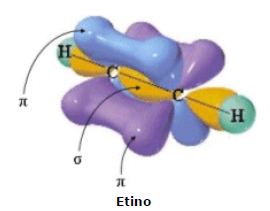
\includegraphics[scale=0.6]{trip}
\end{figure}

Dalla conoscenza della struttura di un triplo legame risulta evidente che il legame $\sigma$ essendo molto corto e localizzato tra gli atomi sarà descritto da delle funzioni p aventi esponente minore rispetto a quelle atte a descrivere la parte $\pi$ del triplo legame, collocata più lontano dagli atomi rispetto alla parte $\sigma$.
Risulta  quindi necessario introdurre un nuovo set di orbitali in aggiunta a quelli della base minima. I set base che raddoppiano in numero di funzioni base vengono definiti a \emph{doppio Zeta} (DZ). Dal momento che queste funzioni aggiuntive sono necessarie solo per la descrizione dei legami chimici si può assumere che lo sdoppiamento degli orbitali di core sia superfluo. Operando lo sdoppiamento solo sugli orbitali di valenza si ottengono i set base \emph{Split-Valence}. Questi ultimi sono sicuramente la categoria di set base più utilizzata e quindi la notazione esplicita VDZ viene ormai spesso omessa in favore della più compatta DZ.
(Non solo di legami covalenti ed elettroni di core vivono le molecole!) Quindi è necessario implementare ulteriori funzioni nel set base che siano in grado di descrivere situazioni più complesse come \emph{legami a idrogeno}, o \emph{doppietti isolati}. Queste situazioni possono essere viste come delle \emph{rotture nella simmetria} degli orbitali. Se quindi si aggiungono ulteriori funzioni con numero quantico superiore a quello concesso dall'atomo ma sottopesate rispetto alle altre, si ottiene un orbitale complessivo \emph{polarizzato}. Questo orbitale a seconda della polarizzazione sarà più adatto a descrivere le diverse situazioni a cui l'atomo può andare incontro rispetto all'orbitale simmetrico. Queste funzioni di polarizzazione sono tipicamente:
\begin{itemize}
\item Orbitali p, per H (Raramente aggiunti, solo se H è coinvolto nella reattività);
\item Orbitali d, per il 2° e il 3° periodo;
\item Orbitali f, per i metalli di transizione;
\item Orbitali g, per il blocco f.
\end{itemize}
Tipicamente vengono aggiunti anche gli orbitali \textit{h} e \textit{i} a partire dai metalli di transizioni in avanti in quanto essi possono dare una varietà di legami particolari che verrebbero descritti approssimativamente dalla sola aggiunta degli orbitali f. 
Queste funzioni di polarizzazione sono fondamentali se si fa uso di metodi che descrivono la correlazione elettronica. Infatti permettono di modificare la forma di orbitali simmetrici in modo da dislocare anisotropicamente gli elettroni nello spazio, dando così una migliore descrizione della correlazione elettronica dinamica. Tipicamente non è un bene aggiungere troppe funzioni di polarizzazione in quanto si va a sbilanciare la forma dell'orbitale. Una regola empirica per mantenere un set base \emph{bilanciato } è quella di andare a ridurre di 1 il numero di funzioni di polarizzazione per ogni nuovo momento angolare aggiunto, ovvero: 
\begin{center}
3s 2p 1d oppure 5s 4p 3d 2f 1g \\ 
e non: \\
3s 2p 2d 2f 1g  \\
\end{center}
Per quanto riguarda la gerarchia dei set base, essa è tipicamente collegata a quante volte un set base viene sdoppiato. Si osserva che la gerarchia emerge spontaneamente dal calcolo di una specifica proprietà (tipicamente l'energia) con diversi set base.

\begin{figure}[H]
\centering
\caption{Andamento dell'energia al variare del set base, con metodi diversi.}\label{oz}
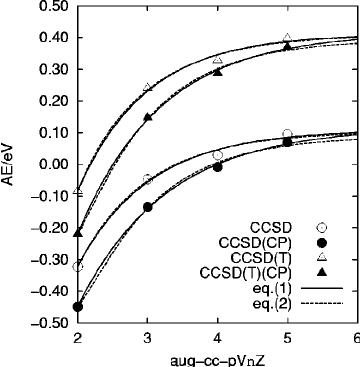
\includegraphics[scale=0.6]{ndz}
\end{figure}

Ovviamente il valore assoluto della proprietà osservata varia a seconda del metodo usato per calcolarla ma l'andamento rispetto al set base rimane invariato per tutti i metodi. Si può notare in figura \ref{oz} che oltre un certo livello di sdoppiamento il valore della proprietà calcolata non subisce ulteriori variazioni. Risulta quindi superfluo effettuare calcoli con set base più complessi in quanto si è già raggiunto il \emph{limite del set base completo}.

\section{Costruzione di set base}
Quando si fa uso di funzioni gaussiane bisogna necessariamente costuire le funzioni atomiche come combinazione lineare di gaussiane, in quanto una simile combinazione lineare è più aderente alla fisica del sistema. Definiamo, quindi le funzioni base di questa combinazione lineare come \emph{gaussiane primitive}, mentre la gaussiana risultante sarà una \emph{gaussiana contratta}.

\subsection{Esponenti di funzioni primitive}
Gli esponenti di queste gaussiane esprimono l'estensione radiale dell'orbitale, infatti esponenti elevati comporteranno delle gaussiane con picchi molto alti adatti a descrivere elettroni molto localizzati, mentre esponenti più bassi saranno funzioni più diffuse utili a descrivire il comportamento lontano dal nucleo.
La determinazione di questi esponenti può passare attraverso il fitting a funzioni STO o possono essere ottenuti variazionalmente minimizzando l'energia di un atomo isolato.
Ciò non si applica alle funzioni di polarizzazione  in quanto essendo orbitali vuoti non contribuiscono all'energia. Una simile minimizzazione dell'energia può essere fatta solo a livello CISD includendo tali orbitali nelle eccitazioni.

\subsection{Set base con esponenti parametrizzati}
Si può notare dall'analisi di set base ottimizzati variazionalmente che il rapporto tra gli esponenti di due gaussiane successive resta pressocché costante.
Si può sfruttare questo fatto per costruire un modello di dipendenza lineare tra l'esponente e dei parametri mantenuti costanti e determinare gli esponenti successivi in base a questo modello. I set base così generati vengono definiti \emph{Even Tempered}:
\begin{equation}
\zeta_i=\alpha\beta^i \quad i=1,2,\ldots,m
\end{equation}
Con questi metodi è facile ottenere un set base che converge al set base completo, tuttavia tale convergenza è lenta e un grande numero di funzioni base vanno utilizzate. Dato che presentano un'efficienza comparabile a quella di un set base ottimizzato a un determinato livello, sono poco utilizzati.
Un'efficienza migliore viene ottenuta ottimizzando parametricamente gli esponenti dei soli orbitali di valenza, metodi che adottano questa tecnica sono detti \emph{Well Tempered}.
\subsection{Set base contratti}\index{Set Base !contratti}
Alla base di questa categoria di set base c'è l'idea che solo gli orbitali di valenza siano coinvolti nella reattività e quindi utili a definire le proprietà interessanti di un sistema. Di conseguenza invece di ottimizzare variazionalmente i coefficienti della combinazione lineare di primitive costituenti il nucleo si procede in tal senso solo con gli orbitali di valenza.
I set base costruiti in questo modo vengono chiamati \emph{contratti} e presentano un'elevata efficienza computazionale a scapito di un aumento di energia dovuto alla scarsa flessibilità del set base.
I set base contratti si possono suddividire in $2$ categorie:
\begin{itemize}
\item \textbf{Segmentati}: L'insieme di gaussiane primitive viene diviso in sottogruppi, ognuno dei quali viene utilizzato per formare un'unica gaussiana contratta. Se la stessa gaussiana primitiva deve essere utilizzata per due gaussiane contratte, una situazione comune, essa dovrà essere sdoppiata aumentando il costo computazionale;
\item \textbf{Generali}: Tutte le gaussiane primitive possono essere utilizzate per costruire qualsiasi gaussiana contratta, ovviamente con coefficienti diversi.
\end{itemize}

\begin{figure}[H]
\centering
\caption{Schema di costruzione di gaussiane contratte segmentate e generali.}\label{coz}
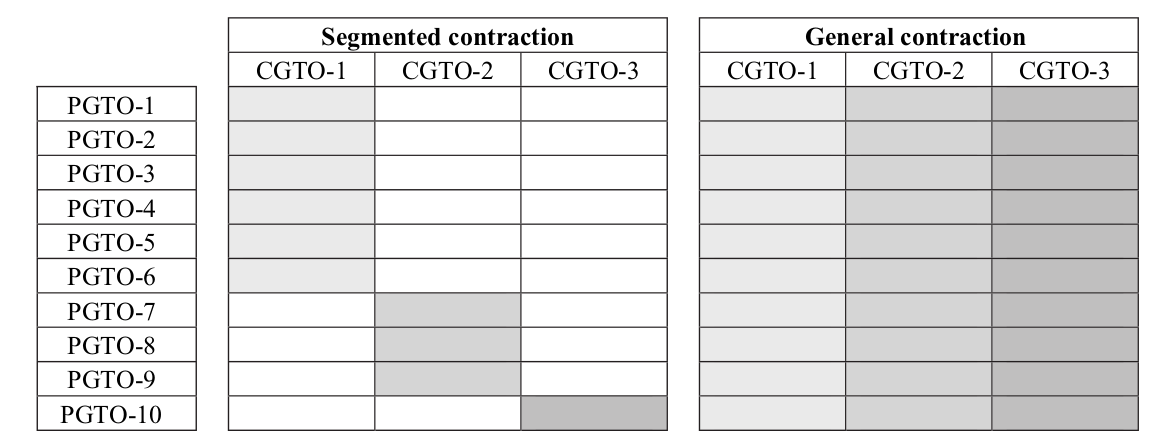
\includegraphics[scale=0.3]{segcon}
\end{figure}

Attualmente quasi tutti i set base utilizzati sono di tipo generale poichè convergono più rapidamente nonostante i set base contratti primitivi convergano a un valore più corretto. I set base contratti sono tipicamente usati con metodi post-HF nei quali il calcolo degli integrali sul set base è una parte minoritaria del tempo di calcolo.

\subsection{Set base aumentati}\index{Set Base !aumentati}

Alcune proprietà molecolari, per una corretta simulazione, necessitano di alcune funzioni aggiuntive rispetto quelle fornite dal set base ottimizzato. Sovente tali proprietà dipendono dalla coda delle funzioni base, spesso scarsamente rappresentata, mentre altre volte dipendono dalla densità elettronica sul nucleo, anch'essa con una rappresentazione insufficiente nei set base classici. Vengono quindi aggiunte alcune funzioni con le caratteristiche necessarie alla simulazione.
I set base che includono queste funzioni si definiscono \emph{aumentati} (aug). Spesso  a causa dell'elevato costo computazionale che questi set base comportano si eliminano alcune funzioni aumentate ottenendo gradi di aumento minori indicati con i mesi dell'anno andando indietro da agosto (jul-, jun-,  may-, ...)
\section{Effective Core Pseudopotential ECP\index{ECP}}
Modellizzare gli atomi più pesanti presenta una serie di problemi, in primo luogo gli elettroni di core non possono più essere descritti dalla semplice meccanica quantistica, in quanto le elevate energie a cui sono sottoposti impongono un trattamento relativistico dei loro moti. In secondo luogo la correlazione statica tra guscio di valenza e guscio interno diventa importante e non può più essere trascurata. Sebbene gli elettroni di core non siano importanti dal punto di vista chimico, il loro effetto si ripercuote anche sul guscio di valenza. Per dare una descrizione dettagliata del guscio interno in modo da descriverne accuratamente l'effetto sugli elettroni di valenza, è necessario utilizzare un'enorme quantità di funzioni base. Così facendo l'efficienza computazionale di qualsiasi metodo crolla e tutto il tempo viene impiegato per calcolare integrali tra orbitali di core invece che essere impiegato per descrivere il più utile guscio di valenza.
Questi problemi possono essere risolti contemporaneamente applicando intorno al nucleo una funzione che modellizzi il contributo medio degli elettroni di core. Una tale funzione prende il nome di \emph{Effective Core Potential ECP} oppure \emph{Pseudo Potenziale PP}.\index{Pseudo Potenziale}
Quando si progetta uno Pseudo Potenziale si seguono i seguenti passaggi:
\begin{enumerate}
\item Si genera una funzione di tutti gli elettroni a partire da un HF numerico o uno corretto per l'equazione di Dirac.
\item Si sostituiscono gli orbitali di valenza con degli pseudo orbitali senza nodi nella parte di core.
\item Si sostituiscono gli orbitali di core con un'espansione di gaussiane o altre funzioni che descrivano il comportamento medio degli elettroni di core, inclusi i contributi relativistici.
\item Si impostano i parametri di questo Pseudo potenziale in modo da garantire che la risoluzione dell'equazione di Dirac\index{Dirac} produca degli pseudo orbitali di valenza. Questi parametri dipendono dal tipo di hamiltoniano impiegato, quindi per ogni hamiltoniano devono essere riottimizzati. Ciò non viene fatto per i metodi DFT perché i diversi hamiltoniani impiegati producono variazioni infinitesime sui parametri che vengono, quindi, assunti costanti.
\end{enumerate}
Per poter effettuare conti con pseudopotenziali bisogna apportare una leggera modifica all'hamiltoniano dividendolo in una parte, che calcola l'energia di valenza, che resta invariata e una parte che calcola l'energia del PP:
\begin{equation}
\hat{H}= \hat{H}_0 +\hat{H}_{PP}
\end{equation}
Costruendo adeguatamente l'hamiltoniano si garantisce l'ortogonalità della parte di valenza con quella di core.

\begin{figure}[H]
\centering
\caption{Diversi esempi di PP indicati come Small e Large comparati con la funzione di tutti gli elettroni.}\label{ecoz}
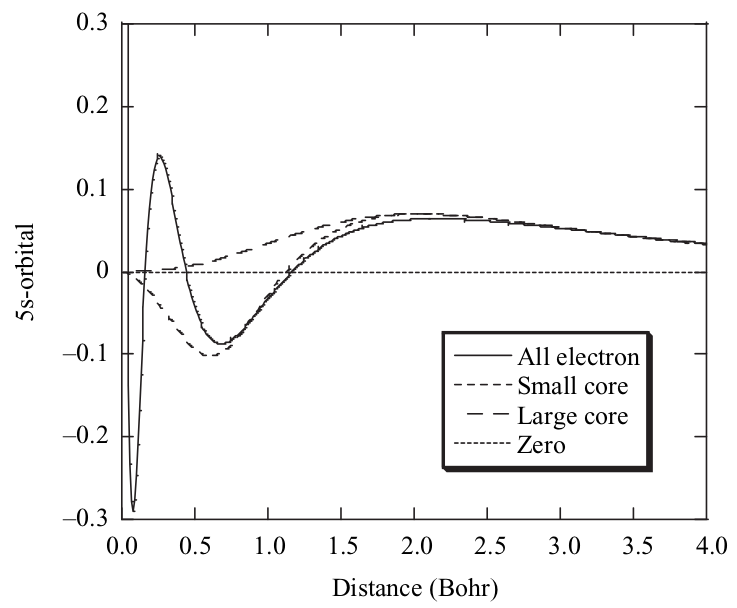
\includegraphics[scale=0.3]{ecp}
\end{figure}

A seconda del sistema analizzato si utilizza un set diverso di funzioni per costruire l'ECP. Nel caso di sistemi molecolari si prediligono le gaussiane, mentre in sistemi solidi l'approccio predominante prevede l'uso di onde piane. Risulta particolarmente importante utilizzare lo stesso tipo di funzioni base usate nella valenza al fine di mantenere \emph{l'ortogonalità tra i due gusci}.

Questo approccio non può essere applicato per proprietà che dipendono direttamente dagli elettroni sul nucleo, come le costanti di schermo NMR.



\section{Basis Set Superposition Error \index{BSSE}}
I set base sono inevitabilmente fonte di errore in quanto non possono essere \emph{completi}. Questo errore è facilmente trattabile in quanto se si sceglie un set base bilanciato esso rimane costante e nel calcolo delle differenze energetiche scompare. 
Tuttavia un secondo errore più subdolo caratterizza i set base. Esso si verifica quando gli orbitali localizzati sui nuclei di due parti interagenti contribuiscono l'una alla densità elettronica dell'altra. Immaginiamo due molecole d'acqua interagenti mediante \textit{legame a idrogeno}, se gli orbitali sull'ossigeno vengono percepiti anche dall'idrogeno dell'altra molecola essi contribuiranno a risolvere l'incompletezza del set base dell'idrogeno, e allo stesso modo faranno gli orbitali sull'idrogeno con l'ossigeno. Fisicamente questa sovrapposizione non avviene  e il risultato sarà quindi un'energia di interazione tra le due molecole d'acqua più bassa rispetto al dato sperimentale. Questo effetto viene chiamato BSSE (\emph{Basis Set Superposition Error}).
Questo tipo di errore risulta particolarmente importante nella trattazione dei \emph{legami deboli}, infatti il sistema di riferimento è la formazione di un dimero:
\begin{center}
A + B $\rightleftharpoons$ AB
\end{center}
Tutti i metodi che propongono una risoluzione del BSSE si attengono a questo modello di reattività.
\subsection{Metodi di risoluzione del BSSE}
Esistono sostanzialmente $3$ metodi per risolvere il problema del BSSE:
\begin{enumerate}
\item \textbf{CounterPoise CP}\index{CounterPoise CP}: Il BSSE viene stimato come differenza tra l'energia dei due monomeri separati con il set base del dimero ($ab$) e l'energia dei due monomeri ognuno con il proprio set base ($a$ e $b$).
\begin{equation}
\begin{aligned}
\Delta E_{complex} &= E(AB)_{ab}^* - (E(A)_a+E(B)_b) \\ \\
\Delta E_{CP} &= (E(A)^*_{ab}+E(B)_{ab}^*) - (E(A)_a+E(B)_b)
\end{aligned}
\end{equation}
Nella seconda equazione si nota che l'energia dei monomeri nella prima parentesi viene calcolata considerando anche il set base della seconda molecola senza che gli atomi di questa siano realmente presenti. Questo particolare set di orbitali viene chiamato \emph{set di orbitali fantasma}
\item \textbf{Chemical Hamiltonian Approach CHA}: \index{Chemical Hamiltonian Approach CHA} Il contributo del BSSE viene escluso a priori dal metodo stesso. Tuttavia l'hamiltoniano diventa \emph{non hermitiano} e i risultati sono analoghi a quelli del CP. Pertanto viene poco usato.
\item \textbf{Bound Function BF}:\index{Bound Function BF} Questo metodo non risolve il problema del BSSE ma migliora la descrizione dell'interazione intermolecolare aggiungendo delle funzioni con esponenti bassi in mezzo alle posizioni atomiche.
\end{enumerate}
\section{Esempi di set base}
Di seguito vengono elencate le principali caratteristiche dei set base più utilizzati. \`E importante ricordare che i set base possono essere costruiti secondo la propria esigenza, pertanto non ci si deve limitare nella scelta del set base\index{set base} a quelli qui elencati, o in generale a quelli preconfezionati.
\subsection{Pople \index{Set Base !di Pople}}
Sono tutti a \emph{contrazione segmentata}, e ne esistono $2$ categorie:
\begin{itemize}
\item \textbf{STO-$n$G}: Sono costituiti da STO formati da $n$ gaussiane primitive. Gli esponenti delle gaussiane primitive sono calcolati per \emph{fitting} sul STO e non ottimizati.
\item \textbf{$k$-$nlm$G}: Sono di tipo \emph{split valence}. Il numero prima del trattino indica quante gaussiane primitive sono utilizzate nella descrizione del core mentre i numeri dopo il trattino indicano quante gaussiane primitive sono impiegate nella descrizione della parte di valenza.
Si possono aggiungere funzioni diffuse tra parentesi dopo la G di gaussiane, come in: 6-311G(d,p) che indica l'aggiunta di orbitali d a tutti gli atomi e p all'idrogeno. L'aggiunta di funzioni aumentate si indica con dei "+" prima della G.
Esponenti e coefficienti di contrazione sono ottimizzati variazionalmente.
\end{itemize}

\begin{figure}[H]
\centering
\caption{Esempi di set base in stile Pople.}\label{popopo}
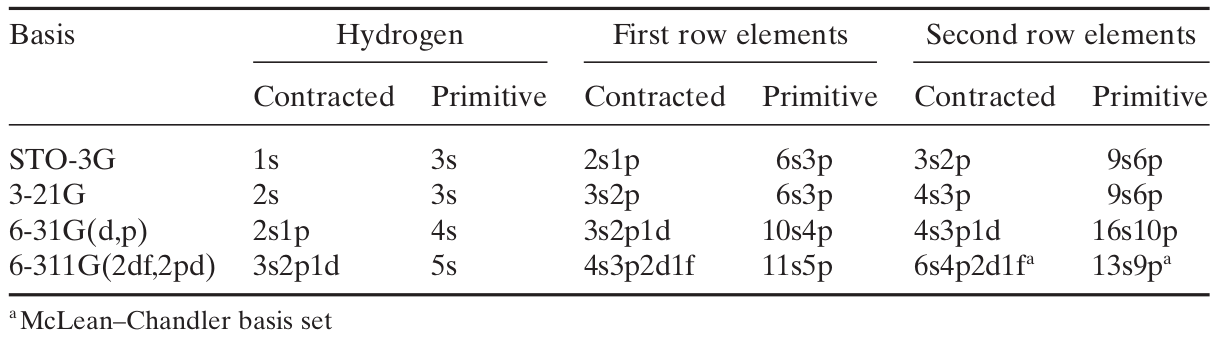
\includegraphics[scale=0.3]{pop}
\end{figure}


\subsection{Dunning-Huzinaga\index{Set Base !di Dunning}}
Sono tutti a \emph{contrazione segmentata}. Sono più flessibili rispetto ai set base di Pople ma utilizzati raramente.

\subsection{Karlsruhe-Type\index{Set Base !di Karlsruhe}}
Sono tutti a \emph{contrazione segmentata}.
Sono computazionalmente molto efficienti ed esistono per tutti gli elementi della tavola periodica, infatti vengono molto usati.

\begin{figure}[H]
\centering
\caption{Esempi di set base in stile Karlsruhe.}\label{popoppppo}
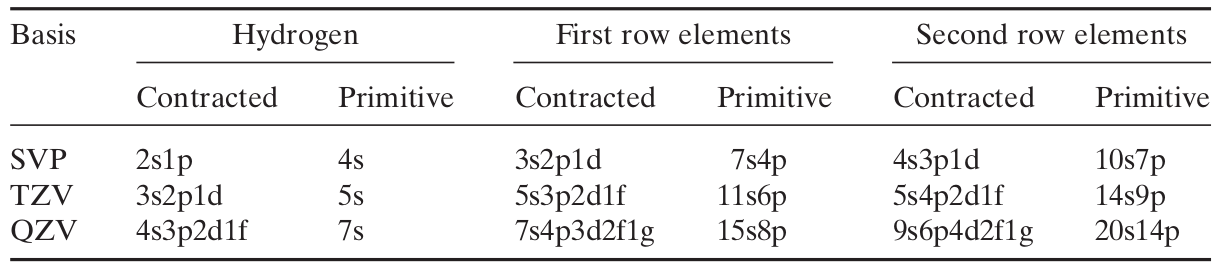
\includegraphics[scale=0.3]{kar}
\end{figure}


\subsection{Atomic Natural Orbitals ANO's \index{Set Base !di ANO}}
Sono tutti a \emph{contrazione generale}. L'idea è di ridurre il numero di gaussiane primitive descrivendo gli orbitali come \emph{orbitali che diagonalizzano la matrice densità  } per un atomo isolato a un livello di teoria elevato (CISD o CASPT2). $$C^\dagger DC=\Lambda$$ I set base così ottenuti sono automaticamente bilanciati ma non esistono per tutti gli atomi (fino al Kr). A causa dell'enorme numero di gaussiane primitive utilizzate nell'ottimizzazione dell'atomo isolato questi set base risultano  molto inefficienti. Sono stati, quindi, proposti dei set base che garantiscono lo stesso livello di accuratezza degli ANO's ma con un costo computazionale minore, ovvero i cc-.

\subsection{Correlation Consistent cc-\index{Set Base !correlation consistent}}
Sono tutti a \emph{contrazione generale}. Il nome correlation consistent significa che orbitali che descrivono circa la stessa quantità di energia di correlazione sono aggiunti insieme nello stesso passaggio. Gli esponenti di orbitali s e p sono ottimizzati a livello HF, mentre i momenti angolari superiori sono otimizzati a livello CISD. Ogni passaggio di aggiunta di orbitali cambia il nome del set base aggiungendo una Z.

\begin{figure}[H]
\centering
\caption{Esempi di set base correlation consistent.}\label{poccpopo}
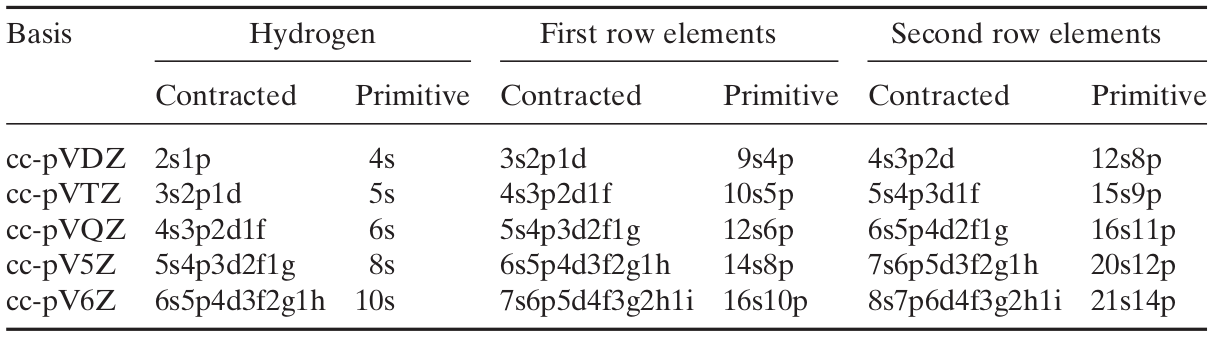
\includegraphics[scale=0.3]{cc}
\end{figure}

Questi set base possono essere modificati aggiungendo una funzione della distanza intermolecolare in modo da dare una descrizione più corretta delle interazioni coulombiane. Questi set base prendono in nome cc-pV$n$Z-F12


\subsection{Polarization consistent pc-\index{Set Base !Polarization consistent}}
Dal momento che i metodi di correlazione hanno andamenti della convergenza al variare dei momenti angolari diversi dai metodi DFT o HF, sono stati sviluppati, parallelamente ai metodi cc-, i metodi pc- adatti esplicitamente per DFT e HF.
Il nome viene assegnato in base a quante funzioni di polarizzazione vengono aggiunte e sono, infatti, spesso utilizzati per valutare l'effetto di un singolo tipo di funzione. Sono stati sviluppati anche in versione \emph{segmentata}, decisamente più efficienti di quelli a contrazione generale.

\begin{figure}[H]
\centering
\caption{Esempi di set base polarization consistent.}\label{crop}
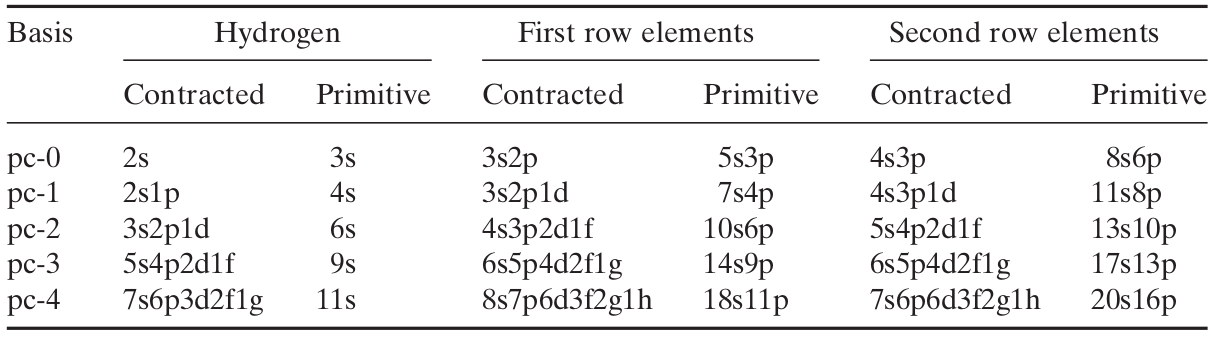
\includegraphics[scale=0.3]{pc}
\end{figure}

\subsection{Relativistici \index{Set Base !relativistici}}
Il metodo più classico per ottenere questi set base è ri-contrarre le funzioni base di un set base non relativistico utilizzando un metodo relativistico.

\section{Funzioni base di Onde piane \index{Set Base !di onde piane} \index{onde piane}}
Per sistemi infiniti, gli orbitali molecolare coalescono in bande, poiché la differenza di energia tra livelli distinti svanisce. Gli elettroni in una banda possono essere descritti da orbitali espansi in un set base di \emph{onde piane}, \index{onde piane} le quali in $3$ dimensioni possono essere scritte come funzioni complesse:
\begin{equation}
\chi_k(r)= e^{ikr}
\end{equation}
Il vettore onda $k$ ricopre lo stesso ruolo dell'esponente $\zeta$ in una base gaussiana ed è correlato all'energia dall'equazione \ref{aaa}.
\begin{equation}
\label{aaa}
E=\frac{1}{2}k^2
\end{equation}
Allo stesso tempo il vettore onda $k$ può essere anche considerato come un fattore di frequenza: alti valori di $k$ indicano oscillazioni rapide. I valori permessi di $k$ sono dati dal vettore di traslazione della cella unitaria $t$. $$kt=2\pi m \quad m\in \mathbb{N}^+$$
Il numero di onde piane ($m_{PW}$) è, perciò, determinato dal vettore $k$ a più alta energia, che definisce implicitamente il massimo di energia cinetica ($E_{max}$) e il volume della cella unitaria ($V$).
\begin{equation}
\label{vess}
m_{PW}= \frac{1}{2\pi^2}V E_{max}^{3/2}
\end{equation}
\`E possibile costruire una gerarchia di set base di onde piane, aumentando il parametro $E_{max}$. Inoltre è possibile notare dall'equazione \ref{vess} che il numero massimo di onde piane da utilizzare per un qualsiasi sistema non dipende dalla natura del sistema ma dall'energia cinetica e dal volume della cella periodica. Ciò è in contrasto con la crescita lineare delle dimensioni del set base con le dimensioni del sistema tipico di set base gaussiani: per sistemi di grandi dimensioni, i set base di onde piane dimostrano un'efficienza maggiore.
Si possono utilizzare set base di onde piane anche per calcoli molecolari, tuttavia in questi casi è necessario utilizzare una \emph{supercella}. In questo modo se la cella è sufficientemente grande due molecole in celle diverse non saranno in grado di interagire e il calcolo sarà sufficientemente accurato. Questo approccio non è applicabile a sistemi carichi o estremamente polari.
Le funzioni base di onde piane sono ideali per descrivere densità elettroniche delocalizzate che variano lentamente come le bande di conduzione e di valenza di un metallo. Tuttavia gli elettroni di core sono estremamente localizzati sui nuclei e perché venga mantenuta la condizione di ortogonalità con la banda di valenza, le onde piane che descrivono quest'ultima devono avere un $k$ molto elevato. Di conseguenza anche l'energia massima aumenterà e con essa il numero di onde piane da inserire nel set base. Questa difficoltà nel modellizzare l'interazione tra elettroni di core e nucleo può essere superata facendo uso di PP.
In conclusione, i set base di onde piane descrivono con precisione i sistemi metallici con elettroni delocalizzati ma offrono una scarsa descrizione della parte di core. Analogamente i set base gaussiani descrivono accuratamente i sistemi periodici molecolari ma introducono un errore significativo nella descrizione della banda di valenza di sistemi metallici.
La soluzione sarebbe l'utilizzo di un sistema misto, in cui la parte di core viene modellizzata da un set base gaussiano mentre la banda di valenza da uno di onde piane. Tuttavia gli integrali misti tra i due tipi di funzioni sono estremamente difficili da valutare e la complessità computazionale rende impraticabile quest'opzione.


\chapter{Teoria del funzionale della densità}
\section{La densità elettronica \index{densità elettronica}}
Hohenberg\index{Hohenberg-Kohn} e Kohn nel 1964 hanno dimostrato che esiste una relazione biunivoca tra l'\emph{energia di un sistema} e la \emph{densità elettronica}, questo fatto è intuitivamente comprensibile se si considera che\index{DFT}
\begin{enumerate}
\item L'integrale della densità elettronica\index{densità elettronica} è il  numero di elettroni del sistema;
\item Le cuspidi nella densità elettronica indicano la presenza di un nucleo;
\item L'altezza delle cuspidi corrisponde alla carica nucleare.
\end{enumerate}
La densità elettronica nell'approccio di Hohenberg e Kohn viene collegata al concetto di \emph{funzione d'onda}. Infatti se una funzione d'onda di $N$ elettroni contiene $4N$ variabili possiamo definire la sua densità elettronica come la densità di probabilità di trovare l'elettrone in una certa regione di spazio:
\begin{equation}
\rho(r) = \int \limits_0 ^{N-1} \vert \Psi(r_i, \sigma_i) \vert ^2 dr \quad i=1,\ldots, N
\end{equation}
Il grande vantaggio della densità elettronica è che la dimensionalità viene sensibilmente ridotta da $4N$ a $3$ indipendentemente dalle dimensioni del sistema.
Inoltre la densità elettronica gode di alcune importanti proprietà:
\begin{enumerate}
\item \`E sempre sempre positiva;
\item Dipende solo da 3 variabili spaziali;
\item All'infinito vale $0$;
\item Il suo integrale è il numero di elettroni;
\item È un'osservabile fisica ottenibile da esperimenti di raggi X;
\item I punti di massimo sono solo in presenza dei nuclei, quindi è definita dalla geometria del sistema;
\item sul nucleo ha il comportamento cuspoidale esatto, legato alla carica nucleare ($Z_A$) da: $$\lim_{r_{iA}\rightarrow 0}\left[ \frac{\partial}{\partial r}+2 Z_A \right] \bar{\rho}(r)=0 $$
con $\bar{\rho}(r)$ la media sferica della densità elettronica;
\item Decade con un andamento esponenziale asintotico a 0.
\end{enumerate}
Tra queste proprietà possiamo individuarne $3$ che definiscono univocamente l'energia elettronica del sistema, ricordando la forma funzionale dell'hamiltoniano in equazione \ref{hamil}. Questi elementi sono:
\begin{itemize}
\item Numero di elettroni;
\item Cariche nucleari;
\item Geometria del sistema.
\end{itemize}
Dato che sia l'energia, sia la densità elettronica dipendono da questi $3$ fattori possiamo affermare che l'energia dipenda dalla densità elettronica secondo una relazione funzionale:
\begin{equation}
E=E[\rho(N,Z_A,R_A)]
\end{equation}
Questa relazione molto importante prende il nome dei primi che riuscirono a dimostrarne la validità. Viene quindi definito \textbf{Primo teorema di Hohenberg-Kohn}.
Il \textbf{Secondo teorema di Hohenberg-Kohn}, afferma invece che l'energia dello stato fondamentale è variazionale rispetto a cambiamenti della densità elettronica
Il problema principale è che pur sapendo che ogni densità elettronica è collegata a un solo stato fondamentale, il funzionale\index{funzionale} che lega queste due quantità non è noto.  Diventa 	quindi di cruciale importanza riuscire a definire un tale funzionale come un'insieme di operazioni che applicate alla densità elettronica restituiscano le proprietà d'interesse.
Di seguito andremo a indagare alcune proposte di teorie atte a descrivere il funzionale tra energia e densità elettronica.
\section{Approccio senza orbitali\index{DFT !senza orbitali}}
Dal confronto con i princ\^ipi di meccanica ondulatoria risulta evidente che il funzionale della densità elettronica debba essere diviso in $3$ parti:
\begin{enumerate}
\item $T[\rho]$ Energia cinetica;
\item $E_{ne}[\rho]$ Potenziale attrattivo elettroni-nuclei;
\item $E_{ee}[\rho]$ Potenziale repulsivo elettrone-elettrone.
\end{enumerate}
La repulsione tra nuclei non viene inclusa dato che si opera entro i limiti dell'approssimazione di Born-Oppenheimer.\index{Born-Oppenheimer}
Iniziamo definendo il potenziale repulsivo elettrone-elettrone come formato da un contributo coulombiano e da uno di scambio in analogia con la teoria di Hartree-Fock, in modo da descrivere anche l'energia di correlazione elettronica. \index{Hartree-Fock} Il potenziale attrattivo elettrone nucleo, così come il contributo coulombiano, saranno  espressi in termini classici:
\begin{equation}
\begin{aligned}
E_{ne}[\rho] &= - \sum \limits_a ^{N_n} \int \frac{Z_a(R_a)\rho(r)}{\vert R_a-r \vert}dr\\
J[\rho] &= \frac{1}{2} \int \int \frac{\rho(r')\rho(r)}{\vert r-r' \vert}dr dr'
\end{aligned}
\end{equation}
Mentre i termini cinetico e di scambio devono essere definiti basandosi sull'assunzione che la densità elettronica sia un gas di elettroni quindi sulla teoria di \emph{Thomas-Fermi}(TF): \index{Thomas-Fermi !teoria di}
\begin{equation}
\begin{aligned}
T_{TF}[\rho]&= C_F \int \rho^{5/3}(r)dr \quad C_F=\frac{3}{10} (3\pi^2)^{2/3} \\
K_{D}[\rho]&= -C_X \int \rho^{4/3}(r)dr \quad C_X=\frac{3}{4} \left( \frac{3}{\pi}\right)^{1/3}
\end{aligned}
\end{equation}
Si costruisce quindi il funzionale della densità elettronica come somma di questi diversi contributi. Spesso si esclude il contributo di scambio per semplificare i calcoli, tuttavia se quest'ultimo viene incluso si parla di modello di Thomas-Fermi-Dirac (TFD).
\begin{equation}
E_{TF}[\rho]= T_{TF}[\rho]  + E_{ne}[\rho] +J[\rho]+ K_D[\rho]
\end{equation}
Su questo modello grava un pesante \emph{difetto}, infatti la densità elettronica trattata come gas di elettroni funziona molto bene per modellizzare solidi metallici periodici, ma non per le molecole. Inoltre in questo tipo di trattazione non è incluso il legame chimico, quindi le molecole non potrebbero esistere. Questi problemi sono stati affrontati sviluppando in serie il termine cinetico senza tuttavia riuscire a dare una descrizione del legame chimico.
\section{La teoria di Kohn-Sham\index{Kohn-Sham}}
Il principale problema dell'approccio senza orbitali è la scarsa descrizione dell'energia cinetica che non include la possibilità che si formino legami. Per superare questo problema Khon e Sham proposero la reintroduzione degli orbitali nella definizione di densità elettronica. In questo modo l'energia cinetica poteva essere in parte calcolata esattamente e in parte corretta mediante dei termini aggiuntivi.
Questo approccio comporta una grave perdita in termini di efficienza computazionale, infatti l'energia torna a dipendere da $3N$ coordinate. Tuttavia considerando che costa quanto un HF ma include nel funzionale l'energia di correlazione risulta essere un metodo conveniente.
L'energia cinetica calcolabile esattamente sarà quella derivante da un approccio HF mentre la correzione includerà i contributi di correlazione statica dinamica e di scambio. Al fine di giustificare questo approccio costruiamo un  hamiltoniano dipendente dal grado di interazione tra elettroni $\lambda$.
\begin{equation}
\hat{H}_\lambda  = T +V_{ext}(\lambda)+\lambda V_{ee} 
\end{equation}
Il potenziale esterno nel caso di un sistema reale con elettroni totalmente interagenti ($\lambda=1$) è uguale a $V_{ne}$. Anche per valori intermedi di $\lambda$ si assume che esso valga 1. Nel caso in cui $\lambda=0$ gli elettroni non interagiscono con i nuclei e la soluzione esatta all'equazione di Schr\"odinger è data da un determinante di Slater composto da spin-orbitali molecolari $\phi_i$. Il funzionale di energia cinetica \emph{esatto } è dato da:
\begin{equation}
T_S= \sum \limits_{i=1} ^{N_e} \langle \phi_i \vert -\frac{1}{2} \nabla ^2 \vert \phi_i \rangle
\end{equation}
La S a pedice indica che è ricavata a partire da un determinante di Slater. Questa formulazione dell'energia cinetica è un'approssimazione in quanto valutata per $\lambda=0$. L'energia cinetica esatta si può calcolare facendo uso di orbitali (naturali, NO) ottenuti mediante diagonalizzazione della matrice densità esatta, di cui sono autovettori.
\begin{equation}
\begin{aligned}
T[\rho_{exact}]&= \sum \limits _{i=1}^\infty n_i \langle \phi_i^{NO} \vert  -\frac{1}{2} \nabla ^2 \vert \phi_i ^{NO}\rangle \\
\rho_{exact}&= \sum \limits _{i=1}^\infty n_i \vert \phi_i ^{NO}\vert ^2 \\
N_e&= \sum \limits _{i=1}^\infty n_i\\
\end{aligned}
\end{equation}
La quantità di elettroni in ogni orbitale è rappresentata dal \emph{grado di occupazione} dell'orbitale $n_i$, che è l'i-esimo autovalore della matrice densità e  può variare tra $0$ e $1$. Rappresentare la densità esatta richiede un numero infinito di orbitali naturali e ciò è impossibile dal punto di vista computazionale. Pertanto si approssimerà la densità elettronica come segue:
\begin{equation}
\rho_{appr}= \sum \limits _{i=1}^{Ne} n_i \vert \phi_i \vert ^2
\end{equation}
Adottare questa approssimazione all'interno della formulazione di $T[\rho_{exact}]$ fa sì che i gradi occupazione degli orbitali siano precisamente o 1 o 0. 
Il termine correttivo all'energia cinetica è dovuto al fatto che i gradi di occupazione \emph{reali} degli orbitali naturali possano scostarsi da 0 e 1. Dato che la soluzione approssimata appena ricavata coincide con quella di un HF monodeterminantale possiamo far coincidere l'energia mancante con quella di \emph{correlazione}.
Questa energia mancante può essere inclusa in un termine di \emph{scambio e correlazione} e  un'espressione generale per l'energia DFT può essere rappresentata da:
\begin{equation}
E_{DFT}[\rho] = T_S[\rho]+ E_{ne}[\rho] + J[\rho] + E_{scamb/corr}[\rho]
\end{equation}
Possiamo definire quindi $ E_{scamb/corr}$ come la somma  dell'energia di correlazione cinetica ($A$) e dell'energia potenziale di scambio e correlazione ($B$).
\begin{equation}
E_{corr/scambio}[\rho]  =  \underbrace{(T[\rho]-T_S[\rho])}_A+\underbrace{( E_{ee}[\rho] - J[\rho])}_B
\end{equation}
In conclusione, se lo scopo dei modelli senza orbitali è di approssimare energia cinetica e di scambio e correlazione, nei modelli KS si approssima solo la parte di scambio e correlazione. Inoltre dato che l'energia di scambio e correlazione è circa 10 volte inferiore all'energia cinetica, la teoria KS è decisamente meno sensibile alle inaccuratezze del funzionale rispetto ai modelli senza orbitali. Mentre i modelli senza orbitali sono realmente dei metodi del funzionale della densità (3 variabili), i metodi KS sono modelli a particella indipendante (3N variabili), analogamente alla teoria HF ma decisamente meno complicati dei metodi post-HF.
\section{Matrice di densità ridotta\index{DFT !matrice densità ridotta}}\label{densr}
Le matrici di densità ridotta costituiscono una valida alternativa all'utilizzo della \emph{densità elettronica stessa}. Esse si applicano quando il sistema analizzato può essere descritto in egual modo in due sottospazi vettoriali dello spazio di Hilbert che definisce la funzione d'onda. Tipicamente questo si concretizza quando sia funzioni d'onda monoelettroniche, sia funzioni d'onda bielettroniche possono essere usate come basi dello spazio vettoriale.
Definiamo quindi $2$ matrici di cui le tracce saranno la densità elettronica di elettroni indipendenti in un caso, e quella di coppie elettroniche nell'altro. Entrambe le matrici complessivamente descrivono la totalità della densità elettronica, tuttavia suddividendone i contributi nelle due matrici parleremo di densità \emph{ridotta}.
Gli elmenti della prima matrice, detta anche del primo ordine, saranno definiti dallo scambio di un singolo elettrone da $r_1$ a $r'_1$ come:
\begin{equation}
\gamma_1(r_1,r'_1)= N_e \int \Psi^*( r'_1, r_2, \ldots, r_{N_e})\Psi( r_1, r_2, \ldots, r_{N_e}) dr_2 dr_3 \ldots dr_{N_e}
\end{equation}
Mentre gli elmenti della seconda matrice, detta anche del secondo ordine, saranno definiti dallo scambio di $2$ elettroni simultaneamente da $r_1$ a $r'_1$  e da $r_2$ a $r'_2$ come:
\begin{equation}
\gamma_2(r_1,r'_1,r_2,r'_2)= N_e(N_e-1) \int \Psi^*( r'_1, r'_2, \ldots, r_{N_e})\Psi( r_1, r_2, \ldots, r_{N_e})  dr_3 \ldots dr_{N_e}
\end{equation}
In queste matrici di densità ridotta non viene incluso lo spin elettronico se non richiesto esplicitamente. Esso può essere introdotto con delle matrici analoge a quelle appena scritte.
La traccia della matrice del primo ordine per $r'_1=r_1$ corrisponde alla funzione di densità elettronica $\rho_1$:
\begin{equation}
\rho_1(r_1) = \gamma_1(r_1,r_1)= N_e \int \Psi^*( r_1, r_2, \ldots, r_{N_e})\Psi( r_1, r_2, \ldots, r_{N_e}) dr_2 dr_3 \ldots dr_{N_e}
\end{equation}
Il termine $N_e$ assicura che l'integrazione avvenga sul numero di elettroni, mentre l'integrale corrisponde alla densità di probabilità di trovare l'elettrone nella coordinata $r_1$.
Per la matrice di densità del secondo ordine avremo la densità di \emph{doppietti elettronici} considerando $r'_1=r_1$ e $r'_2=r_2$:
\begin{equation}
\rho_1(r_1, r_2) = \gamma_2(r_1,r_1,r_2,r_2)= N_e(N_e-1) \int \Psi^*( r_1, \ldots, r_{N_e})\Psi( r_1, \ldots, r_{N_e})  dr_3 \ldots dr_{N_e}
\end{equation}
Il termine $N_e(N_e-1)$ assicura l'integrazione sul numero di doppietti elettronici, mentre il termine nell'integrale è la probabilità di trovare due elettroni, uno in $r_1$ e uno in $r_2$.
Da queste matrici è possibile ricavare le energia cinetica e potenziale esatte:
\begin{equation}
T=-\frac{1}{2} \int \nabla^2 \gamma_1(r_1r'_1) \vert_{r=r'}dr_1
\end{equation}
Mentre l'energia potenziale va suddivisa in un contributo monoelettronico $V_{ne}$ e uno bielettronico $V_{ee}$:
\begin{equation}
\begin{aligned}
V_{ne} &=- \sum \limits_A ^{N_n} \int \frac{Z_A \gamma_1(r_1,r_1)}{\vert R_A-r_1\vert} d r_1\\
V_{ee} &=  \frac{1}{2} \int \frac{\gamma_2(r_1,r_1,r_2,r_2)}{\vert r_1 -r_2\vert} dr_1 dr_2
\end{aligned}
\end{equation}
L'energia potenziale può essere riscritta in termini di $\rho_1$ e $ \rho_2$, quindi solo l'energia cinetica richiede la conoscenza della matrice di densità del primo ordine.
Nel caso di una funzione d'onda monodeterminantale come quella di HF le matrici di densità ridotta si riducono a:
\begin{equation}
\gamma_1(r_1,r'_1) = \sum \limits_{i=1} ^{Nocc} \phi_i(r'_1)\phi_i(r_1)
\end{equation}
\begin{equation}
\gamma_2(r_1,r'_1,r_2,r'_2)=\sum \limits_{i,j=1} ^{Nocc} \{\phi_i(r'_1)\phi_j(r'_2)\phi_i(r_1)\phi_j(r_2)-\phi_i(r'_1)\phi_j(r'_2)\phi_j(r_1)\phi_i(r_2)\}
\end{equation}
Dove i $\phi_m(r_n)$ sono gli spin-orbitali del determinante di Slater.
Utilizzando queste definizioni delle matrici di densità ridotta nelle definizioni delle energie potenziali e cinetica si ottiene l'espressione dell'energia di Hartree-Fock.
Dato che la matrice del primo ordine può essere ricavata per integrazione diretta della matrice del secondo ordine, possiamo pensare di utilizzare gli elementi della matrice del secondo ordine per risolvere l'equazione di Schr\"odinger in modo variazionale. Purtroppo tali elementi non possono variare liberamente poichè devono corrispondere a una funzione d'onda asimmetrica. Questo problema si definisce di N-rappresentabilità, e si può risolvere obbligando la matrice di densità a due particelle $\gamma_2$ o $D$, e le sue rappresentazioni in termini di particella-hole $Q$ e hole-hole $G$ a essere \emph{semidefinite positive}, in quanto queste matrici devono descrivere una probabilità. L'ottimizzazione di queste matrici scala come $m^6$ ed è quindi fattibile per buona parte dei sistemi.
La qualità dei risultati è comparabile con quella di un metodo CCSD(T) ma più tollerante rispetto sistemi intrinsecamente multiconfigurazionali. 
In generale questi metodi si differenziano dai post-HF per i seguenti motivi:
\begin{enumerate}
\item Nei post-HF si usa l'hamiltoniano esatto ma si approssima la funzione d'onda;
\item I metodi DFT approssimano il funzionale dell'energia ("hamiltoniano") ma permettono una libera variazione della densità elettronica. La definizione del funzionale deve imporre la N-rappresentabilità e ciò si verifica naturalmente nei metodi KS mentre deve essere esplicitato nei metodi senza orbitali;
\item  Nei metodi senza orbitali il funzionale dell'energia cinetica non è noto e una minima inaccuratezza  genera risultati totalmente sbagliati. Mentre nei funzionali KS non si conosce una piccola parte dell'energia cinetica dovuta a correlazione e scambio e gli effetti sull'energia finale sono minori.
\item I metodi che usano $\gamma_1$ come variabile possono imporre strettamente la condizione di N-rappresentabilità, impiegando il funzionale di energia esatta per tutti i termini eccetto quello di correlazione. Quest'ultimo termine dipende da $\gamma_2$ che, in questo approccio, dipende da $\gamma_1$;
\item I metodi che usano $\gamma_2$ come variabile impiegano il funzionale di energia esatta in termini di $\gamma_2$, ma quest'ultimo deve essere approssimato per imporre la N-rappresentabilità di $\gamma_2$;
\item I metodi che usano $\rho_2$ come variabile usano un funzionale di energia esatta per le interazioni elettrone-nucleo e elettrone-elettrone. Tuttavia devono approssimare sia l'energia cinetica, sia imporre la N-rappresentabilità di $\rho_2$.
\end{enumerate}
\section{Potenziale di scambio e correlazione}
Dobbiamo esprimere l'energia di scambio e correlazione come un funzionale della densità elettronica. Ma poiché la parte di scambio è la parte preponderante di questo contributo possiamo pensare di calcolarla esattamente a partire dagli orbitali attraverso la formula:
 \begin{equation}
 E^{HF}=\sum \limits_{i=1} ^{N}  \hat{h}_{i} + \frac{1}{2} \sum \limits_{i=1} ^{N} \sum \limits_{j=1} ^{N}  (J_{ij}-K_{ij}\delta_{\sigma_i \sigma_j})+\langle V_{nn}\rangle
 \end{equation}
Di questa equazione si calcola esattamente il contributo di scambio mentre la correlazione viene calcolata con un metodo DFT.
Tuttavia questo approccio dà risultati poveri se si fa uso di orbitali KS in quanto il potenziale diventa non locale.
Ciò comporta che  l'energia di correlazione statica nei metodi HF cancella il contributo dell'energia di correlazione dinamica mentre nei metodi DFT le definizioni di queste due parti essendo locali non permettono un'accurata descrizione del sistema.
Consideriamo quindi l'energia di scambio come una correzione quantistica alla classica repulsione tra elettroni e includiamo in essa anche un contributo di autointerazione. Il termine di scambio, già presente nella teoria HF, deve essere, quindi, incluso nel DFT considerando anche un effetto dinamico di repulsione interelettronica che aumenta il contributo energetico del HF. Questo contributo in più è assimilabile all'energia di correlazione calcolata con metodi post-HF.
Tutte queste considerazioni possono essere modellizzate in termini di \emph{buchi di probabilità}: se gli elettroni fossero privi di carica o spin la probabilità di trovare un elettrone sarebbe indipendente dalla posizione di un altro elettrone, e la densità di doppietti elettronici sarebbe data dal semplice prodotto di due densità monoelettroniche a meno di un fattore di normalizzazione. 
\begin{equation}
\rho_2^{indip} (r_1, r_2) = \frac{N_e -1}{N_e}\rho_1(r_1) \rho_1(r_2)
\end{equation}
Dato che però gli elettroni sono dotati di carica e spin questa trattazione deve essere modificata per includere la repulsione interelettronica. La modifica consiste nell'aggiungere ai termini già presenti una correzione:
\begin{equation}
\rho_2(r_1, r_2) = \rho_1(r_1) \rho_1(r_2)+ \rho_1(r_1) h_{corr/scam}(r_1, r_2)
\end{equation}
con:
\begin{equation}
 h_{corr/scam}(r_1, r_2)= \frac{ \rho_2(r_1,r_2)}{ \rho_1(r_1)}- \rho_2(r_2)
\end{equation}
Da questa trattazione emerge che il contributo alla buca di scambio è dovuto esclusivamente a elettroni con spin uguali e coincide, quindi, con la \emph{buca di 
Fermi.} mentre la parte di correlazione essendo dovuta alla repulsione coulombiana prenderà il nome di \emph{buca di Coulomb}. 
La principale differenza con il metodo HF sta nel fatto che le buche di scambio HF sono delocalizzate su tutta la molecola in quanto contributo non locale mentre nella teoria DFT esse sono localizzate con precisione, ciò non permette la cancellazione dell'autointerazione coulombiana come nell'HF. Nessun funzionale DFT fin'ora creato riescie a cancellare l'autointerazione coulombiana in modo completo come nel metodo HF.


\section{Funzionali di scambio e correlazione}
Le principali differenze tra i funzionali DFT risiedono nella definizione della parte di scambio e correlazione. Sebbene sia stato provato che un funzionale universalmente valido per tutti i sistemi esista esso non è ancora stato individuato. Tuttavia si possono definire alcune proprirtà che un simile funzionale deve possedere:
\begin{enumerate}
\item Deve essere privo di contributi di autointerazione coulombiana, ovvero il contributo di scambio deve cancellare perfettamente il contributo coulombiano;
\item Per densità elettroniche costanti si deve ottenere come risultato un gas di elettroni uniforme. Questa condizione risulta più importante per sistemi di stato solido piuttosto che per sistemi molecolari;
\item L'energia di scambio deve essere lineare rispetto le coordinate della densità elettronica, ovvero moltiplicano un fattore a ogni coordinata di $\rho$ e applicando il funzionale si deve ottenere che: $$E_x[\rho_\lambda] = \lambda E_x[\rho] $$
\item l'energia di correlazione non deve scalare linearmente con le coordinate elettroniche;
\item Se il fattore di scaling va a infinito l'energia di correlazione deve assumere un valore negativo;
\item L'energia di scambio e correlazione non può superare il valore massimo imposto dalla legge di \emph{Lieb- Oxford}\index{Lieb-Oxford !legge di};
\item L'energia di scambio deve valere $-r^{-1} $ per $r\rightarrow\infty$;
\item L'energia di correlazione deve valere $-1/2\alpha r^{-4}$ con $\alpha$ che è la polarizzabilità di un sistema $N_e-1$
\end{enumerate}
A causa delle differenze nello scaling dei contributi scambio e correlazione essi vengono spesso trattati separatamente nei funzionali che quindi verranno espressi come:
\begin{equation}
E_{xc}[\rho]= E_{x}[\rho] + E_{c}[\rho] =\int \rho(r) \varepsilon_x[\rho(r)]dr + \int \rho(r) \varepsilon_c[\rho(r)]dr
\end{equation}
Dato che il termine di scambio coinvolge solo particelle con lo stesso spin esso sarà dipendente dalle densità elettroniche di spin separatamente, mentre la parte di correlazione dovrà includere dei termini che mescolano le densità elettroniche di spin differenti:
\begin{equation}
\begin{aligned}
E_{x}[\rho]&= E_{x}^\alpha[\rho_\alpha] + E_{x}^\beta[\rho_\beta]\\
E_{c}[\rho] &= E_{c}^{\alpha\alpha}[\rho_\alpha] + E_{c}^{\beta\beta}[\rho_\beta] + E_{c}^{\alpha\beta}[\rho_{\alpha},\rho_\beta ]
\end{aligned}
\end{equation}
In sistemi a gusci chiuso le due densità di spin si equivalgono. Per i sistemi paramagnetici dato che la distribuzione di spin è polarizzata, i funzionali di scambio e correlazione vengono espressi in termini di polarizzazione di spin:
\begin{equation}
\zeta=\frac{\rho_{\alpha}-\rho_{\beta}}{\rho_{\alpha}+\rho_{\beta}}
\end{equation}
Per i metodi DFT non è possibile definire un parametro in base al quale costruire gerarchicamente dei nuovi funzionali. Tuttavia Perdew nel 2001 ha proposto una scala di efficienza dei funzionali basata sull'accordo con i dati sperimentali chiamata \emph{scala di Giacobbe}.
\subsection{Local Density Approximation LDA \index{LDA}}
Nel metodo LDA  si assume che la densità localmente possa essere trattata come un gas di elettroni \emph{uniforme}, quindi in grado di variare lentamente.
L'energia di scambio si definisce come:
\begin{equation}
E_x^{LDA} [\rho] = -C_x \int \rho ^{4/3}(r) dr
\end{equation}
Questa formula si riferisce a una sola densità elettronica, introducendo i contributi di due popolazioni di spin separate diventa:
\begin{equation}
E_x^{LDA} [\rho] = -C_x \int \rho_\alpha ^{4/3}(r)+\rho_\beta ^{4/3}(r) dr
\end{equation}
Per sistemi  a guscio chiuso quest'ultima formula si riduce a quella senza spin, infatti si parla indiscriminatamente di LDA o LSDA.
L'ultima formula si può esprimere anche in termini di $\zeta$.
L'energia di correlazione in questo metodo è stata calcolata ai limiti per densità elevate, e per densità basse. Per i casi intermedi è stata quantificata numericamente mediante metodi Monte Carlo\index{Monte Carlo}.
Questo metodo è totalmente inadatto alla modellizzazione di molecole o cristalli molecolari e trova spazio solo nella comunità di fisici dello stato solido che modellizzano sistemi metallici.
\subsection{Generalized Gradient Approximation GGA \index{GGA}}
In questo tipo di modello si considera la densità elettronica come un gas di elettroni \emph{non uniforme}, in termini di funzionale esso dipenderà anche dal gradiente della densità elettronica. questa dipendenza dal gradiente fa sì che spesso i metodi GGA siano considerati \emph{non locali}.
Uno dei funzionali di scambio di questo tipo più famosi è il Becke (B o B88). \index{Becke B}
\begin{equation}
E_x= E_x^{LDA}+\Delta E_x^{B88}
\end{equation}
\begin{equation}
\Delta E_x^{B88}=-\beta \rho^{1/3} \frac{x^2}{1+6\beta x \sinh^{-1}x} \quad \text{con: } x= \frac{\vert \nabla \rho \vert}{\rho^{4/3}}
\end{equation}
La densità elettronica corretta per il suo gradiente ha il comportamento corretto all'infinito per la densità di energia ma non per il potenziale di scambio. Questo metodo permette di ridurre l'errore commesso da un metodo LSDA fino a $2$ ordini di graandezza al prezzo dell'aggiunta di un solo parametro. Esistono funzionali di scambio migliori ma implementano almeno $2$ parametri come nel caso dell'OPTX.
Per quanto riguarda la correlazione sono stati proposti numerosi funzionali diversi. Uno tra i più utilizzati è stato proposto da Lee-Yang-Parr è viene definito LYP.\index{Lee-Yang-Parr LYP} Questo funzionale dipende da $3$ parametri e non contempla la correlazione tra spin accoppiati.
Spesso i funzionali di scambio vengono accoppiati a quelli di correlazione ottenendo funzionali misti denominati come BLYP (B88 + LYP) o OLYP (OPTX + LYP).
Sono stati sviluppati funzionali che includono sia una parte di scambio, sia una di correlazione e che assicurano le integrazioni corrette delle relative buche. Tali funzionali devono i natali a Perdew-Wang (PW86 e PW91) e a Perdew-Burke-Ernzerhof (PBE).\index{PBE} \index{PW86} \index{PW91}Nei funzionali PBE la parte di scambio viene trattata con un fattore moltiplicativo allo scambio LSDA mentre la correlazione come un fattore additivo alla correlazione LSDA:
\begin{equation}
\begin{aligned}
E_x^{PBE} &= E_x^{LDA} F(x) \\
E_c^{PBE} &= E_c^{LDA} + H(t)
\end{aligned}
\end{equation}
Le funzioni $F(x)$ e $H(t)$ dipendono da $4$ parametri $a,b,c,d$ ricavati da dati calcolati.
\subsection{Meta-GGA \index{m-GGA}}
I funzionali m-GGA includono derivate della densità elettronica di ordine superiore. Spesso sostituiscono queste derivate con la densità di energia cinetica orbitalica che dipende direttamente dalla derivata seconda della densità ma l'algoritmo che la calcola è più stabile.
Alcuni di questi funzionali riescono a risolvere il problema dell'\emph{autointerazione coulombiana}.
\subsection{Funzionali Ibridi \index{Funzionali ibridi}}
L'idea guida dei funzionali ibridi sta nell'utilizzare l'energia di scambio esatto HF come componente della parte di scambio.
L'energia di correlazione e scambio diventa quindi una somma pesata di contributi calcolati con diversi metodi, per esempio:
\begin{equation}
E_{xc}=0.5E_x^{HF}+0.5(E_x^{LDA}+E_c^{LDA})
\end{equation}
In questo funzionale le due parti vengono pesate in equal modo e viene quindi chiamato \emph{half-half} (H-H). Funzionali più efficienti sono stati sviluppati con fattori di peso ottimizzati a partire dall'accordo con i dati sperimentali. Il caso più importante è quello del B3LYP\index{B3LYP}, che fa uso di un contributo Becke allo scambio e di uno LYP alla correlazione. Il numero $3$ indica che i pesi ai diversi contributi di scambio e correlazione sono ottimizzati in base a $3$ parametri $a,b,c$ ottenuti per best fit su dati empirici.
\begin{equation}
E_{xc}^{B3LYP}=(1-a)E_x^{LDA}+aE_x^{HF}+b\Delta E_x^{B88}+(1-c)E_c^{LDA}+cE_c^{LYP}
\end{equation}
Grazie all'ottimo accordo con i dati sperimentali che si ottiene facendo uso di questo tipo di funzionali, essi sono in assoluto la tipologia di funzionale più utilizzata. I parametri possono essere agevolmente variati per descrivere delle proprietà particolari e il costo computazionale non supera quello di un normale HF.
Esistono metodi che implementano nella descrizione della correlazione un contributo post-HF, solitamente MP2. Questi metodi richiedono risorse computazionali decisamente superiori a quelle dei semplici ibridi, e sono, quindi, scarsamente impiegati. Quest'ultimo tipo di funzionali prende in nome di \emph{doppiamente ibridi}.
\section{Considerazioni Computazionali}
Analizziamo ora quali siano gli step che ci permettono di ottenere un valore di energia a partire da una qualsiasi definizione del funzionale di scambio e correlazione, e da una qualsiasi scelta di orbitali del set base atti a definire la densità elettronica. 
Una volta operate le suddette scelte il problema si riduce a determinare un set di orbitali ortogonali che minimizzi l'energia, esattamente come nella teoria HF. Possiamo quindi definire una funzione \emph{Lagrangiana}\index{Lagrange !metodo di}:
\begin{equation}
\mathcal{L}[\rho]= E_{DFT}[\rho]-\sum \limits _{ij} ^{N_e} \lambda_{ij}(\langle\phi_i\vert\phi_i\rangle-\delta_{ij})
\end{equation}
Imponendo la condizione di annullamento della Lagrangiana, si ottiene un operatore monoelettronico $h_{KS}$ in perfetta analogia con il metodo HF.
\begin{equation}
\begin{aligned}
h_{KS} \phi_i &= \sum \limits _{j} ^{N_e} \lambda_{ij} \phi_j \\
h_{KS} &= \frac{1}{2} \nabla^2 +v_{eff} \\
v_{eff}&= V_{ne}(r)+\int \frac{\rho (r')}{\vert r-r' \vert} dr' +V_{xc}(r)\\
V_{xc}(r)&= \frac{\delta E_{xc}[\rho]}{\delta \rho(r)}
\end{aligned}
\end{equation}
Il termine di scambio e correlazione si ottiene operando la derivata del funzionale di correlazione e scambio che si ha scelto di utilizzare.
Diagonalizzando la matrice dei moltipicatori di Lagrange si ottiene un set di orbitali ortogonali canonici detti di Khon-Sham definiti da un equazione agli pseudo-autovalori:
\begin{equation}
h_{KS}\phi_i=\varepsilon_i\phi_i
\end{equation}
Questa equazione può essere risolta espandendo gli orbitali KS in termini del set base, ottenendo così l'analogo DFT delle equazioni di Roothaan-Hall\index{Roothaan-Hall !equazioni di}:
\begin{equation}
\begin{aligned}
\phi_i &= \sum \limits_{\mu = 1}^m c_{\mu i }\chi_{\mu} (r-R_A)\\
h_{KS}C &= SC\varepsilon
\end{aligned}
\end{equation}
Queste equazioni vengono risolte analiticamente tranne che nella parte di scambio e correlazione che deve essere valutata numericamente campionando su una serie di punti griglia. Questo tipo di integrazione impone dei limiti in quanto non possono essere fatti confronti tra metodi che usano diverse distribuzioni o diverse quantità di punti griglia. Inoltre il nu non aggiunge vocimero di punti griglia scala linearmente con le dimensioni del sistema e rende molto lunga la valutazione di simili integrali per sistemi di grandi dimesioni.
\section{Difetti dei metodi DFT}
\paragraph{Il teorema di Hohenberg-Kohn\index{Hohenberg-Kohn} assicura che la densità elettronica contenga tutta l'informazione di cui abbiamo bisogno. Tuttavia nell'approssimazione di Khon-Sham consideriamo valida una matrice di densità ridotta troncata al primo ordine. Questa approssimazione potrebbe non valere per sistemi con una gran quantità di correlazione statica\index{correlazione !statica }. Per superare questo problema si sviluppa la matrice di densità ridotta come combinazione lineare di più determinanti di Slater. Si ottengono così i metodi \emph{ensemble DFT}.\\}
 \paragraph{I sistemi radical anionici e radical cationici non vengono descritti bene. Infatti si generano cariche frazionarie e geometrie elongate. Questi problemi sono da imputare alla incompeta cancellazione del contributo di autointerazione coulombiana.\\}
 \paragraph{Le differenze di energia tra stati a diversa molteplicità di spin sono spesso inesatte. Ciò è dovuto ai difetti nella definizione dei funzionali di correlazione e scambio.\\}
 \paragraph{Talvolta componenti isotrope del momento di spin presentano una sensibile anisotropia anche in assenza di campi magnetici esterni. Ciò è dovuto alle differenze di densità elettronica utilizzata per descrivere le diverse componenti. Può essere evitato omogeneizzando la densità elettronica.}
\chapter{Metodi semiempirici}\label{semi}
Nei metodi \emph{ab initio} fin'ora analizzati si cerca il set di funzioni d'onda costituenti il determinante di Slater che minimizza, in senso variazionale, l'energia del sistema. Tale minimizzazione viene svolta risolvendo le equazioni di Roothaan-Hall la cui risoluzione scala formalmente come $m^4$. L'obbiettivo dei metodi semiempirici e ridurre il costo computazionale trascurando parte degli integrali necessari alla risoluzione di tali equazioni.
La prima approssimazione che viene spesso fatta nei metodi semiempirici è trascurare totalmente gli elettroni di core diminuendo artificialmente la carica nucleare. In secondo luogo si opera un'ulteriore approssimazione riducendo il set base alla base minima, tendenzialmente esattamente di tipo Slater.
Il primo metodo sviluppato su cui si sono basati tutti quelli successivi è definito \emph{Zero Differential Overlap ZDO}.
In quest'approssimazione si considera che:
\begin{enumerate}
\item La matrice di overlap coincide con l'identità;
\item Tutti gli integrali con più di 2 centri sono trascurati.
\end{enumerate}
I modi in cui gli integrali vengono esclusi o considerati come costanti definiscono i diversi metodi. 
\section{I metodi NDDO}\index{NDDO}
In questi metodi non vengono svolte ulteriori approssimazioni rispetto quelle sovracitate. Vengono definiti \emph{Neglect of Diatomic Differential Overlap}.
In quest'approssimazione gli integrali di repulsione coulombiana sono calcolati tra due \emph{distribuzioni di carica}.
\begin{equation}
\gamma_{AB} =\langle s_As_B \vert \frac{1}{r_{AB}}\vert s_As_b \rangle
\end{equation}
Calcolando in questo modo i contributi bielettronici resta da definire il contributo monoelettronico in termini di una carica nucleare modificata per il numero di elettroni di core ($Z'_A$):
\begin{equation}
h=-\frac{1}{2}\nabla^2 -\sum \limits _A^{N_n} \frac{Z'_A}{\vert R_A -r \vert}
\end{equation}
Per determinare gli elementi di questo operatore si devono testare tre casistiche moltiplicando a destra e a sinistra per diversi elementi del set base:
\begin{enumerate}
\item A=B, $\mu=\nu$ assume dei valori finiti;
\item A=B, $\mu\neq\nu$ gli elementi di $h$ vanno a $0$;
\item A$\neq$B, $\mu\neq\nu$ vale una delta di Kronecker tra atomi e orbitali.
\end{enumerate}
\section{I metodi INDO}\index{INDO}	
In questa approssimazione vengono trascurati tutti gli integrali bielettronici che non siano coulombiani. Questa approssimazione è intermedia tra la NDDO e la CNDO.
Al fine di mantenere  l'invarianza rotazionale, ovvero l'indipendenza dell'energia dalla rotazione delle coordinate del sistema, gli integrali del tipo sotto illustrato devono essere indipendenti dalla natura degli orbitali che coinvolgono.
\begin{equation}
\begin{aligned}
\langle \mu_A \vert V_A\vert \mu_A \rangle \\
\langle \mu_A \nu_A \vert \mu_A \nu_A \rangle
\end{aligned}
\end{equation}
 La più grande conseguenza di questa approssimazione è la scomparsa degli integrali monoelettronici che coinvolgono orbitali diversi sullo stesso atomo.
\section{I metodi CNDO}\index{CNDO}
In questa approssimazione tutti gli integrali bielettronici sono trascurati. Appartiene a questa categoria il metodo PPP.
\section{La parametrizzazione}
Quando si parla di trascurare gli integrali, in realtà si intende operare una loro parametrizzazione. Infatti l'esclusione completa degli integrali produrrebbe effetti talmente drastici da rendere inutilizzabile qualsiasi metodo semiempirico. Il loro utilizzo resta comunque limitato ai sistemi di dimensionalità eccessiva.
I parametri intendono quindi prendere il posto degli integrali, in tre diversi modi:
\begin{enumerate}
\item Gli integrali rimanenti vengono calcolati a partire dalla forma funzionale degli orbitali atomici;
\item I parametri vengono determinati da dati sperimentali atomici;
\item  I parametri vengono determinati da dati sperimentali molecolari.
\end{enumerate}
La scelta di un particolare metodo per la valutazione degli integrali bielettronici, determina la natura di un \emph{metodo modificato}. Un metodo modificato ha tendenzialmente un'efficienza superiore ai metodi visti fin'ora, ma solo per determinate proprietà.
Di seguito viene proposta una breve lista di approssimazioni modificate:
\begin{enumerate}
\item MNDO: Implementa una diversa definizione del potenziale per legami che coinvolgono l'idrogeno;
\item AM1: È un MNDO con le funzioni per gli orbitali di core modificate e riparametrizzate in modo da descrivere adeguatamente anche interazioni a distanze superiori ai $2-3$ \r{A};
\item PM3: Di fatto è identico a un AM1 con tutti i parametri perfettamente ottimizzati su un vasto set di dati sperimentali;
\item MINDO/3: I parametri sono stabiliti per gli integrali bielettronici in base a coppie di atomi.
\end{enumerate}
\section{I metodi di H\"uckel}\index{H\"uckel}
\subsection{Extended HT}
Nei metodi di H\"uckel tutti gli elementi di ogni matrice vengono parametrizzati. Vengono quindi anche definiti metodi non SCF, poiché non fanno uso di processi iterativi.
Si fa uso di questi metodi solo per stabilire la simmetria degli orbitali o per dare una stima iniziale della matrice densità per calcoli successivi.
Gli elementi della matrice di Fock vengono ricavati a partire dall'energia di ionizzazione ($I_\mu$).
\begin{equation}
\begin{aligned}
F_{\mu\mu}&=-I_\mu \\
F_{\mu\nu}&= -K \left(\frac{I_\mu+I_\nu}{2}\right) S_{\mu\nu}
\end{aligned}
\end{equation}
L'energia del sistema equivale dunque alla somma delle energie monoelettroniche, tale situazione evidentemente non fisica, limita notevolmente l'utilizzo di questi metodi.
\subsection{HT}
Un'ulteriore semplificazione è offerta dalla teoria di H\"uckel pura in cui solo gli orbitali $\pi$ vengono considerati al fine del calcolo mentre gli orbitali $\sigma$ sono di fatto un mero schermo alla carica nucleare.
A causa delle drastiche approssimazioni questo metodo fornisce risultati qualitativamente corretti solo per sistemi planari. Per ulteriori approfondimenti si rimanda al corso di Chimica Fisica II.
\part{Applicazione dei metodi}\label{p3}
\chapter{Termodinamica Statistica}\index{Termodinamica statistica}
Lo scopo principale della termodinamica è di correlare diverse grandezze \emph{macroscopiche} attraverso relazione matematiche. Tuttavia i sistemi ai quali tali grandezze si riferiscono sono, tendenzialmente, formati da un numero molto elevato di "particelle" o, più coerentemente con i nostri scopi, di \emph{entità chimiche}. Si potrebbe dunque immaginare che le osservabili fisiche macroscopiche siano in un qualche modo collegate alle proprietà quantistiche della singola entità chimica che costituisce il sistema analizzato. Tali proprietà quantistiche non dovrebbero più costituire un mistero per i lettori, in quanto tutti i metodi analizzati sin'ora in questo testo permettono il calcolo dell'energia totale e dell'entropia di una singola molecola o di un solido infinito. A partire da queste due semplici variabili termodinamiche è possibile risalire a tutte le proprietà macroscopiche di interesse sperimentale.
Il passaggio dal mondo microscopico a quello macroscopico, tuttavia, non è banale e necessita la conoscenza di strumenti matematici propri sia della meccanica razionale sia della statistica come la ricerca di punti di minimo e massimo mediante il metodo di Lagrange \index{Lagrange !metodo di} o il concetto di valor medio.
\section{Definizioni e concetti preliminari}
Prima di iniziare con una trattazione formale della termodinamica statistica è necessario dare qualche definizione.
In particolare in questo capitolo ogni proprietà termodinamica verrà catalogata come \emph{meccanica} o \emph{non meccanica}, le prime saranno tutte le proprietà il cui calcolo non include la temperatura, mentre le seconde terranno conto del valore della temperatura nella loro definizione. A questo punto la definizione di variabile meccanica o non, dovrebbe risultare molto poco limpida, infatti solo attraverso una definizione statistica di tali proprietà la dipendenza o meno dalla temperatura risulterà evidente, ma per giungere a una tale definizione si dovrà attendere la trattazione formale.
Un secondo concetto che fondamentale definire prima di iniziare la trattazione completa è quello di \emph{ensamble}\index{ensamble}, ovvero di insieme. In questo contesto il termine insieme assume il significato di \emph{collezione di sistemi} ove ogni sistema è una replica termodinamica del macrosistema che si vuole investigare sebbene più piccolo come mostrato in Figura \ref{Arcamadonna}.
Ma definiamo meglio i concetti di \emph{insieme} e \emph{sistema}. L'insieme è l'oggetto termodinamico (in questo contesto sinonimo di \emph{macroscopico}) che intendiamo descrivere, mentre un \emph{sistema} è una sua porzione in un preciso istante di tempo. Si rende necessario definire ora un terzo concetto ovvero quello di \emph{stato quantistico}. Uno \emph{stato quantistico} è una precisa combinazione di funzioni d'onda che caratterizza un sistema. Pertanto uno \emph{stato quantistico} avrà due caratteristiche fondamentali:
\begin{itemize}
\item Sarà uno \emph{stato stazionario} in quanto il sistema è "congelato" a un dato istante di tempo;
\item Sarà un \emph{autostato dell'energia}, è quindi in grado di descrivere \emph{totalmente } le interazioni intermolecolari all'interno del sistema che analizziamo
\end{itemize}
Parallelamente allo \emph{stato quantistico} possiamo individuare anche uno \emph{stato termodinamico} ovvero la particolare combinazione di $V,N,T$ che caratterizza l'insieme in esame. All'interno di un particolare \emph{insieme} possiamo individuare un numero estremamente elevato di \emph{stati quantistici} tuttavia essi non saranno identici tra loro e così le loro energie. Sebbene le energie di diversi \emph{stati quantistici} abbiano teoricamente valori discreti quando il numero di tali stati aumenta si può assumere che le energie varino in modo continuo. Si potrà dunque definire una distribuzione di \emph{stati quantistici} rispetto le energie come mostrato in figura \ref{mxwldis}.
\begin{figure}
\centering
\caption{Esempio di come diverse configurazioni di sistemi possano essere utilizzate per generare un insieme di sistemi.}\label{Arcamadonna}
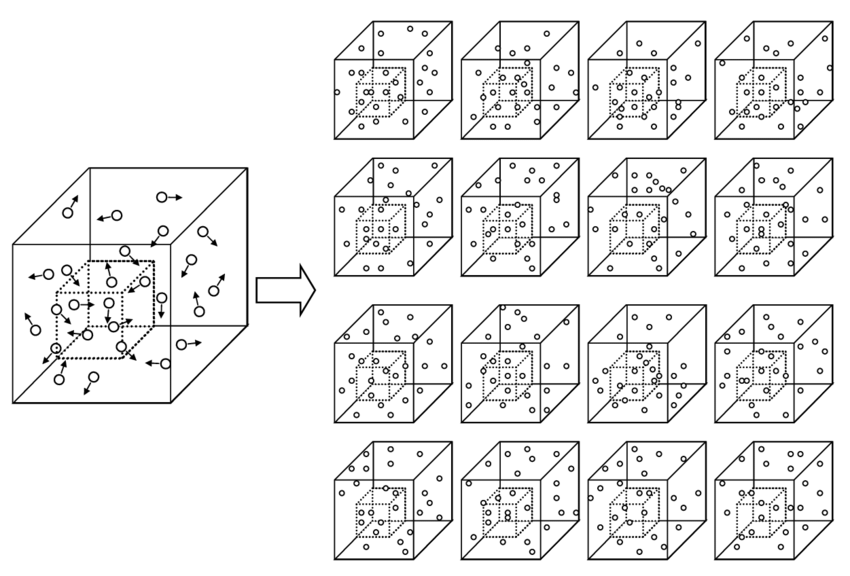
\includegraphics[scale=0.3]{ensamble_gen}
\end{figure}
\subsection{Postulati della termodinamica statistica}
\begin{itemize}
\item La media temporale, su un intervallo di tempo che tende a infinito, di una \emph{variabile meccanica} M del sistema termodinamico analizzato, è uguale alla media della variabile stessa su un insieme infinito di sistemi che sono replica termodinamica di quello in esame (\emph{ensamble}).
\item In un insieme infinito rappresentativo di un sistema isolato termodinamicamente, ogni \emph{stato quantistico} (livello energetico), compatibile con i valori di N (numero di entità chimiche), V (volume del sistema) ed E (energia totale del sistema), è rappresentato con la stessa frequenza o probabilità.
\end{itemize}
Per giungere alla formulazione di questi due postulati ci si è basati sul modello del sistema isolato, tuttavia essi verranno applicati anche per sistemi chiusi e aperti \emph{isotermi} in quanto restano pressocché validi a meno di qualche ridefinizione concettuale dell'insieme stesso.
Nella definizione del secondo postulato viene fatto uso del termine \emph{stato quantistico} che nel contesto di un sistema supramolecolare come il nostro assume lo stesso significato del caso molecolare, sebbene quando il numero di entità aumenta con esso aumentano anche gli stati quantistici. Se ci si pone nel caso in cui in un singolo sistema ci sono centinaia se non migliaia di entità chimiche separate, i singoli stati energetici saranno talmente vicini tra loro da formare di fatto un continuo.
Nella trattazione che segue verranno analizzati i tre insiemi più comuni:
\begin{itemize}
\item Insieme Canonico, corrispondente a un sistema isotermo chiuso;
\item Insieme Grancanonico, corrispondente a un sistema isotermi aperto;
\item Insieme Microcanonico, corrispondente a un sistema isolato.
\end{itemize}
\section{Insieme canonico}
In un insieme canonico i sistemi sono isolati termicamente dall'ambiente esterno e tra loro possono scambiare solo calore, quindi energia. Ciò implica che la temperatura di tutti i sistemi sia costante e che il numero di molecole in un singolo sistema non cambi. Dato che il numero di entità chimiche in un sistema non può cambiare solo alcuni stati energetici saranno accessibili, quindi i sistemi dovranno distribuirsi tra essi secondo una precisa regola matematica detta appunto distribuzione.
Alla stessa energia possiamo trovare una moltitudine di arrangiamenti di sistemi dell'insieme che soddisferanno la distribuzione di sistemi quindi ogni distribuzione di sistemi sarà caratterizzata da una \emph{molteplicità}: 
\begin{equation}
\Omega=\frac{\mathcal{N}!}{\prod_j n_j!}
\end{equation}
Dove $\mathcal{N}$ è il numero di sistemi nell'ensamble, mentre $n_j$ è il numero di sistemi dell'insieme che hanno energia $e_j$.
A partire dai postulati e dalla definizione di ensamble canonico risulta evidente che:
\begin{equation}
\label{Ruzzipippacoca}
\begin{aligned}
E_{tot}&= \sum_j n_je_j\\
\mathcal{N}&= \sum_j n_j
\end{aligned}
\end{equation}
Le relazioni individuate in Eq.\ref{Ruzzipippacoca} costituiscono, inoltre, le condizioni alle quali una distribuzione di sistemi $\bold{n}(e)$ deve sottostare affinché sia rappresentativa del macrosistema isotermo chiuso che si vuole analizzare. In generale la distribuzione dei sistemi può essere diversa da quella \emph{classica} di Maxwell-Boltzmann\index{Maxwell-Boltzman}, infatti nel caso in cui le particelle che costituiscono il sistema non siano atomi o molecole bensì \emph{fermioni} o \emph{bosoni} si dovrà far uso rispettivamente delle distribuzioni di \emph{Fermi-Dirac} e \emph{Bose-Einstein}. \index{Fermi-Dirac} \index{Bose-Einstein}
\begin{figure}[H]
\centering
\caption{Distribuzione dei sistemi su diversi stati energetici secondo Boltzmann.}\label{mxwldis}
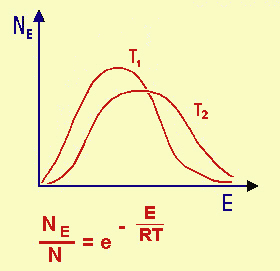
\includegraphics[scale=0.5]{maxwel1}
\end{figure}

In generale, nell'insieme canonico, la probabilità che un certo sistema abbia energia $e_j$ può essere rappresentata dal Eq.\ref{provita}
\begin{equation}
\label{provita}
P_j= \frac{\bar{n}_j}{\mathcal{N}}= \frac{1}{\mathcal{N}}\frac{\sum_\bold{n}\Omega_\bold{n}n_{j\bold{n}}}{\sum_\bold{n}\Omega_\bold{n}}
\end{equation}
In questa equazione la sommatoria $\sum_\bold{n}$ rappresenta una somma su tutti gli elementi della distribuzione, quindi su tutti i possibili arrangiamenti di sistemi che soddisfano le condizioni imposte dalle Eq.\ref{Ruzzipippacoca}
Per definizione di probabilità stessa:
\begin{equation}
\sum_jP_j=1
\end{equation}
La conoscenza della distribuzione di probabilità permette di calcolare le medie sull'insieme delle variabili meccaniche mediante le seguenti equazioni:
\begin{equation}
\begin{aligned}
\bar{E}&=\sum_j P_j\cdot E_j \\
\bar{p}&=\sum_j P_j\cdot p_j
\end{aligned}
\end{equation}
La conoscenza di un'espressione per la probabilità che tenga conto di una dipendenza esplicita dall'energia di un singolo arrangiamento risulterebbe essere molto più comoda rispetto all'equazione \ref{provita}, in quanto l'energia di un singolo arrangiamento è facilmente ottenibile da un calcolo \emph{ab initio} o di \emph{meccanica molecolare}.
Per ottenere questo risultato bisogna riarrangiare l'equazione \ref{provita} utilizzando il \emph{metodo del termine massimo}. \index{termine massimo !metodo del}
\subsection{Metodo del termine massimo}
Nell'approssimazione del termine massimo si assume che operando con numeri molto grandi, dell'ordine del numero di Avogadro, valga la seguente relazione:
\begin{equation}
\lim _{M\rightarrow \infty} \ln\sum_{j=1}^M t_j!=\ln t_{max}!
\end{equation}
Il significato intrinseco di questa approssimazione risiede nel fatto che tra tutti gli \emph{stati energetici} accessibili secondo la distribuzione dei sistemi nelle diverse energie, solo quello con il maggior numero di arrangiamenti possibili, ovvero con la massima molteplicità $\Omega(n^*)$, dominerà nel calcolo della media.
In pratica quella che prima era una distribuzione qualsiasi collassa in una \emph{delta di Dirac}.
La dimostrazione della validità dell'approssimazione del termine massimo è molto semplice se affrontata con la notazione degli O grandi:
\begin{equation}
\begin{aligned}
S&=\sum_{j=1}^M t_j! \\
t_{max}\leq &S \leq Mt_{max} \\
\ln t_{max}\leq &\ln S \leq \ln M + \ln t_{max} \\
t_{max}&= O(e^M)\\
\text{lnM è trascurabile} &\text{ rispetto a M per sistemi grandi}\\
O(M) \leq &\ln S \leq O(M)\\
\ln S&= \ln t_{max}
\end{aligned}
\end{equation}
\subsection{Derivazione della probabilità}
Possiamo riprendere ora la definizione di probabilità in Eq.\ref{provita} e passare al logaritmo in modo da poter applicare il metodo del termine massimo sulla molteplicità, eliminando così la sommatoria:
\begin{equation}
P_j= \frac{1}{\mathcal{N}}\frac{\Omega^*n_{j}^*}{\Omega^*}=\frac{n_{j}^*}{\mathcal{N}}
\end{equation}
Tuttavia il problema viene solamente spostato, infatti ora bisogna trovare lo stato energetico che, pur soddisfacendo le condizioni delle Eq.\ref{Ruzzipippacoca}, massimizza la sua degenerazione. Ciò è possibile farlo mediante il metodo dei moltiplicatori indeterminati, ovvero una massimizzazione con vincoli in cui non si conoscono i moltiplicatori di Lagrange.\index{Lagrange !moltiplicatori di}
Dato che il logaritmo di una funzione è monotono con la funzione stessa possiamo massimizzare il logaritmo della degenerazione per motivi di convenienza matematica in quanto utilizzando ladefinizione di degenarazione iniziale è possibile applicando l'approssimazione di Stirling giungere a un'espressione molto semplice: \index{approssimazione di Stirling}
\begin{equation}
\ln \Omega_\bold{n}= \ln \mathcal{N}! - \sum_k \ln n_k!= \mathcal{N} \ln \mathcal{N} - \mathcal{N}- \sum_k n_k\ln n_k + \sum_k  n_k = \mathcal{N} \ln \mathcal{N}- \sum_k n_k\ln n_k 
\end{equation}
Il risultato appena ottenuto ci tornerà utile in un secondo momento, procediamo ora con la massimizzazione con vincoli:
\begin{equation}
\begin{aligned}
\frac{\partial}{\partial n_j}\left[\ln \Omega_\bold{n} - \alpha_k \left(\sum_k  n_k -\mathcal{N}\right) -\beta \left(\sum_k  n_k E_k - E_{tot} \right)\right] &=0\\
\frac{\partial}{\partial n_j}\left[\mathcal{N} \ln \mathcal{N}- \sum_k n_k\ln n_k  - \alpha_k \sum_k  n_k -\alpha_k\mathcal{N} -\beta \sum_k  n_k E_k - \beta E_{tot}\right] &=0\\
\frac{\partial}{\partial n_j}\left[- \sum_k n_k\ln n_k  - \alpha_k \sum_k  n_k -\beta \sum_k  n_k E_k \right] &=0\\
-n_j \frac{1}{n_j} -\ln n_j -\alpha_k -\beta E_j &=0 \\
\text{applicando: } \alpha+1&=\alpha^\prime\\
 -\alpha^\prime-\beta	E_j&= \ln n_j \\
 e^{ -\alpha^\prime-\beta	E_j} &= n_j ^*
\end{aligned}
\end{equation}
Abbiamo così ottenuto una forma analitica del termine massimo della distribuzione di sistemi, a meno dei due moltiplicatori di Lagrange.\index{Lagrange !moltiplicatori di}
\subsection{Determinazione dei moltiplicatori di Lagrange}
In questo paragrafo deriveremo esclusivamente il parametro $\alpha$, in quanto la derivazione del parametro $\beta$ non è banale è richiede conoscenze matematiche approfondite, pertanto verrà fornito direttamente il risultato e una spiegazione informale del procedimento.
\subsubsection{Determinazione di $\alpha$}
\begin{equation}
\sum_j n_j^* = e ^{-\alpha} \sum_j e^{-\beta E_j} \quad \quad  e ^{-\alpha} =\frac{\mathcal{N}}{\sum_j e^{-\beta E_j}}
\end{equation}
Reinserendo la definizione di $e ^{-\alpha}$ nella prima equazione si ottiene:
\begin{equation}
 n_j^* = \mathcal{N}\frac{ e^{-\beta E_j}}{\sum_j e^{-\beta E_j}} 
\end{equation}
Da cui deriva che la probabilità assume la forma:
\begin{equation}
\label{partizione}
P_j= \frac{ n_j^*}{\mathcal{N}} = \frac{ e^{-\beta E_j}}{\sum_j e^{-\beta E_j}} 
\end{equation}
L'equazione \ref{partizione} costituisce uno dei più importanti risultati in chimica-fisica, infatti per la prima volta la probabilià con cui uno stato energetico si palesa viene correlata all'energia stessa dello stato. Quanto più è grande la probabilità e tanto più sarà piccolo il denominatore, il quale risulta essere di estrema importanza, guadagnadosi il nome di \emph{funzione di partizione}. \index{funzione di partizione}
\begin{equation}
Q=\sum_j e^{-\beta E_j}
\end{equation}
\subsubsection{Determinazione di $\beta$}
Per poter determinare il valore di $\beta$ bisogna in primo luogo definire una \emph{forma differenziale} per l'energia:
\begin{equation}
\begin{aligned}
d\bar{E}&=\sum_j E_j dP_j + \sum_j P_j dE_j\\
&= -\frac{1}{\beta}\sum_j \left(\ln P_j+ \ln Q\right)dP_j + \sum_j P_j \left(\frac{\partial E_j}{\partial V}\right)_N dV 
\end{aligned}
\end{equation}
Operando una serie di trasformazioni si giunge alla seguente espressione:
\begin{equation}
-\frac{1}{\beta}d\left(\sum_j P_j \ln P_j\right)= d\bar{E}+\bar{p}dV
\end{equation}
Da una ben nota corrispondenza termodinamica sappiamo che:
\begin{equation}
TdS=dE+pdV
\end{equation}
Da cui possiamo dedurre che:
\begin{equation}
TdS\leftrightarrow -\frac{1}{\beta}d\left(\sum_j P_j \ln P_j\right)
\end{equation}
Inoltre:
\begin{equation}
\label{satto}
dS \leftrightarrow \frac{1}{\beta T}dG
\end{equation}
Quindi:
\begin{equation}
G=-\sum_j P_j \ln P_j
\end{equation}
Il primo membro di Eq.\ref{satto} è un differenziale esatto, quindi anche il secondo membro lo deve essere. Questa condizione viene soddisfatta solo se $\beta $ è una funzione qualsiasi di G.
Ma ricordando che l'energia libera di Gibbs è additiva, con la conseguenza che deve valere:
\begin{equation}
\frac{df(G_A)}{dG_A}=\frac{df(G_B)}{dG_B}
\end{equation}
L'unica funzione che non cambia al variare della variabile di differenzazione e che mantiene la condizione di additività è una \emph{costante} $k$.
Quindi possiamo riscrivere la probabilità come:
\begin{equation}
P_j= \frac{ n_j^*}{\mathcal{N}} = \frac{ e^{-E_j/kT}}{\sum_j e^{- E_j/kT}} 
\end{equation}
La costante $k$ è stata determinata sperimentalmente, e assume il valore della costante di Boltzmann.
\subsection{Derivazione dell'equazione fondamentale dell'insieme canonico}
A partire dalla nuova definizione di probabilità possiamo definire l'energia libera di Gibbs, e successivamente determinare l'entropia
\begin{equation}
G= -\sum_j P_j \ln P_j; \quad \quad S=kG
\end{equation}
Svolgendo i calcoli per l'entropia si ottiene:
\begin{equation}
S=-k\left[\sum_j P_j \left(-\frac{E_j}{kT}-\ln Q (N,V,T) \right) \right]
\end{equation}
Riscrivendo come la media sull'energia e moltiplicando all'interno $k$ si ottiene:
\begin{equation}
S= \frac{\bar{E}}{T} +k \ln  Q (N,V,T); \quad A=U-TS; \quad A=-kT \ln  Q (N,V,T)
\end{equation}
L'ultima equazione è la relazione fondamentale dell'insieme canonico. Ogni volta che si ootiene una relazione simile ci si può ricondurre dunque all'insieme canonico.
\section{Insieme Grancanonico}
Quando si parla di insieme grancanonico ci si riferisce a un insieme di sistemi immersi in un bagno termico quindi a temperatura costante, ma in grado di scambiare materia tra loro. In questo insieme, quindi il numero di particelle in un sistema non è più costante bensì il potenziale chimico, ovvero l'energia libera di Gibbs molare, non varierà. Ciò implica che il sistema analizzato è un sistema in equilibrio sia termico che chimico aperto.
Le condizioni che bisogna imporre a questo insieme cambiano leggermente da quelle imposte al canonico, sebbene per semplicità manterremo la stessa notazione
\begin{equation}
\begin{aligned}
\mathcal{N}&=\sum_{j,N} n_j(N)\\
N_{tot} &= \sum_{j,N} N_jn_j(N)\\
E_{tot}&= \sum_{j,N} e_jn_j(N)
\end{aligned}
\end{equation}
Si può notare come venga aggiunta la condizione che il numero totale di molecole del macrosistema non cambi mentre si permette il libero scambio di entità chimiche tra i sistemi aggiungendo la dipendenza della distribuzione dal numero di molecole $\bold{n}(e,N)$ e imponendo tale dipendenza facendo correre le sommatorie anche su un indice di numero di molecole.
In un procedimento analogo a quello svolto per l'insieme canonico si deve ricercare la massima degenerazione degli stati (arrangiamenti), e per fare ciò si assegnano tre moltiplicatori di Lagrange alle tre condizioni: $\alpha$ alla prima, $\beta$ alla seconda e $\gamma$ alla terza.
\begin{equation}
n^*_j(N) = e^{-\beta e_j(N,V)}e^{-\gamma N}e^{-\alpha}
\end{equation}
Da cui deriva che sommando su j e su N si ottiene la funzione di partizione per l'insieme grancanonico:
\begin{equation}
\Xi =\sum_{j,N}e^{-\beta e_j(N,V)}e^{-\gamma N}
\end{equation}
\subsection{Determinazione dei moltiplicatori di Lagrange}
La funzione di partizione ricopre lo stesso ruolo di quella nel canonico, è quindi fondamentale per calcolare la probabilità di uno stato e con essa i valori medi delle variabili meccaniche.
Si può ora sfruttare nuovamente la forma differenziale dell'energia per ottenere un'espressione corretta del valore dei moltiplicatori di Lagrange. \index{Lagrange !moltiplicatori di}
\begin{equation}
\begin{aligned}
d\bar{E} &= \underbrace{\sum_j P_j (N) dE_j}_{pdV}+\underbrace{\sum_j E_j dP_j(N)}_{X} \\
X= -\frac{1}{\beta}&\left[ \sum_{j,N} \ln P_j(N)dP_j(N) + \sum_{j,N}\gamma N d P_j(N)+\ln \Xi d \sum_{j,N}P_j (N)\right] \\
\sum_{j,N} E_j dP_j (N) &=-\frac{1}{\beta}\left[ \sum_{j,N} \ln P_j(N)dP_j(N) + \gamma  d \bar{N}\right]\\
d\left[ \sum_{j,N}P_j(N) \ln P_j(N)\right]&= \sum_{j,N} \ln P_j(N)dP_j(N) + \sum_{j,N}P_j(N)\frac{1}{P_j(N)} dP_j(N)\\
\end{aligned}
\end{equation}
Quindi tornando alla forma differenziale dell'energia possiamo riscrivere:
\begin{equation}
d\bar{E }= p\bar{p}dV-\frac{\gamma}{\beta}d\bar{N }- \frac{1}{\beta} d \left[ \sum_{j,N}P_j(N) \ln P_j(N)\right]
\end{equation}
Ovvero riarrangiando:
\begin{equation}
\underbrace{- \frac{1}{\beta} d \left[ \sum_{j,N}P_j(N) \ln P_j(N)\right]}_{TdS}=d\bar{E}+\bar{p}dV+\underbrace{\frac{\gamma}{\beta}d\bar{N}}_{-\mu dN}
\end{equation}
DA cui possiamo dedurre che:
\begin{equation}
\beta=\frac{1}{kT};\quad \quad \gamma= -\frac{\mu}{kT}
\end{equation}
\subsection{Derivazione dell'equazione fondamentale dell'insieme grancanonico}
Come per il caso dell'insieme canonico impostando le relazioni per l'entropia e per la probabilità ci si può ricavare l'equazione fondamentale dell'insieme grancanonico.
\begin{equation}
S= k  \sum_{j,N}P_j(N) \ln P_j(N); \quad \quad P_j(N)=\frac{e^{-\frac{E_j}{kT}}e^{\frac{\mu N}{kT}}}{\Xi}
\end{equation}
Quindi passando ai logaritmi della seconda equazione si ottiene:
\begin{equation}
\ln P_j(N) = -\frac{E_j}{kT}+\frac{\mu N}{kT}-\ln \Xi
\end{equation}
Si può quindi inserire quest'ultimo risultato nell'espressione dell'entropia:
\begin{equation}
S= -k \left[ -\frac{\bar{E}}{kT}+ \frac{\mu \bar{N}}{kT}-\ln \Xi\right]= \frac{\bar{E}}{T}-\mu \frac{ \bar{N}}{T}+k\ln \Xi\end{equation}
Passando a sinistra dell'uguale la funzione di partizione si ottiene:
\begin{equation}
\label{cin}
kT \ln \Xi = TS - \bar{E} + \mu\bar{N}
\end{equation}
Ricordando le varie relazioni che intercorrono tra le funzioni di stato termodinamiche è possibile ottenere l'equazione fondamentale dell'insieme grancanonico:
\begin{equation}
\begin{aligned}
G&=H-TS\\G&=U+pV-TS\\\mu N&=U+pV-TS\\TS&=U+pV-\mu N
\end{aligned}
\end{equation}
Correlando l'ultima equazione con l'espressione ricavata in Eq.\ref{cin} si ottiene infine l'equazione caratteristica dell'insiemo grancanonico ovvero:
\begin{equation}
kT\ln \Xi=pV
\end{equation}
\section{Insieme Microcanonico}
Un insieme microcanonico è rappresentativo di un sistema isolato isotermo, quindi tutti i sistemi all'interno dell'insieme avranno $N$, $V$, $E$ costanti. Ovvero lo stesso volume conterrà lo stesso numero di molecole e quindi lo stesso valore di energia sarà accessibile a tutti i sistemi. Questo caso coincide, di fatto, con un insieme canonico degenere in cui si sono eliminati tutti i sistemi che differiscono in energia dal valore medio.
Possiamo sfruttare la degenerazione dell'insieme canonico nel microcanonico per cercare di ricavare la funzione di partizione di quest'ultimo. In questo caso non è possibile utilizzare lo stesso procedimento adottato negli altri due casi in quanto l'esistenza di una forma differenziale sull'energia implica che questa non sia costante, e ciò vìola gli assunti di partenza.
La prima variabile termodinamica, nonché l'unica ottenibile dall'insieme canonico, è l'entropia. Prima però è necessario ricavarsi la probabilità per un insieme microcanonico:
\begin{equation}
P_j= \frac{e^{-\frac{E_j}{kT}}}{\sum_j e^{-\frac{E_j}{kT}}}=  \frac{e^{-\frac{E}{kT}}}{\Omega e^{-\frac{E}{kT}}}
\end{equation}
Dato che l'energia è uguale in tutti i sistemi si può tranquillamente sostituire la sommatoria con la degenerazione.
Inserendo il termine a destra dell'equazione nella definizione di entropia si ottiene:
\begin{equation}
S=-k\sum_j P_j \ln P_j=-k\Omega\frac{1}{\Omega}\ln\frac{1}{\Omega}=k\ln\Omega
\end{equation}
L'ultima equazione a destra è un risultato fondamentale della termodinamica statistica dovuto a Boltzmann che correla l'entropia alla disponibilità di stati energetici accessibili. Grazie a questa relazione si è potuto affermare che l'entropia sia una sorta di misura del "disordine" di un sistema.
Oltre a questo importantissimo risultato risulta lampante il fatto che tutte le sommatorie sui vari stati saranno sostituite dalla molteplicità dell'unico stato, ovvero che sarà impossibile ottenere un'espressione per un'ipotetica funzione di partizione, infatti per l'insieme microcanonico \emph{non esiste} una funzione di partizione.
Ora sorge la necessità di ricavarsi le altre funzioni termodinamiche, ciò è possibile farlo grazie all'espressione per l'entropia e ricordando che l'energia  è degenere.
\begin{equation}
\begin{aligned}
\frac{1}{kT}&=\frac{\partial\ln\Omega}{\partial E}\biggr\rvert_{V,N}\\\frac{p}{kT}&=\frac{\partial\ln\Omega}{\partial V}\biggr\rvert_{E,N}\\-\frac{\mu_i}{kT}&=\frac{\partial\ln\Omega}{\partial N_i}\biggr\rvert_{E,V,N_{\alpha\neq i}}\end{aligned}
\end{equation}
\section{Fluttuazioni}
Fin'ora abbiamo discusso di come a patire da una distribuzione di probabilità sia possibile ricavarsi diverse variabili termodinamiche senza approfondire la natura della distribuzione stessa. In questo paragrafo vogliamo ricavare una definizione termodinamica della varianza della distribuzione, in modo da individuarne l'entità in relazione al valor medio.
Definiamo quindi \emph{fluttuazione} l'ordine di grandezza della varianza della distribuzione.
Risulta evidente che non tutte le variabili possono fluttuare, in particolare solo quelle che sono definite univocamente per ogni particolare \emph{stato quantistico} ovvero le \emph{variabili meccaniche}. Inoltre nei diversi insiemi le variabili che restano costanti sono diverse e così quelle che possono fluttuare, ne consegue che per insiemi diversi avremo fluttuazioni di variabili diverse.
Per i nostri scopi indageremo esclusivamente le fluttuazioni dell'energia in un insieme canonico e quelle di $N$ in un insieme grancanonico.
\subsection{Fluttuazioni di $E$}
Nella breve intoduzione di questo paragrafo si è dato per scontato il fatto che lo "sparpagliamento" di una distribuzione possa quantificarsi mediante la \emph{varianza}, tuttavia ciò è vero solo per le distribuzioni gaussiane, ma dato che operiamo su sistemi di dimensioni paragonabili al numero di Avogadro possiamo essere sicuri, per la legge dei grandi numeri, che la distribuzione sia gaussiana.
Scriviamo ora la completa derivazione termodinamica della deviazione standard dell'energia:
\begin{equation}
\sigma_E=\left[\overline{\left(E-\bar{E}\right)^2}\right]^{1/2}= \left[ \bar{E^2}-(\bar{E})^2\right]^{1/2}
\end{equation}
Data la seguente equazione:
\begin{equation}
\bar{E}\sum_j e^{-\frac{E_j(N,V)}{kT}}=\sum_j E_j(N,V) e^{-\frac{E_j(N,V)}{kT}}
\end{equation}
Possiamo derivare entrambi i lati dell'uguale per T:
\begin{equation}
\frac{\partial\bar{E}}{\partial T}\biggr\rvert_{V,N}\underbrace{\sum_je^{-\frac{E_j}{kT}}}_{Q}+\frac{\bar{E}}{kT^2}\sum_jE_je^{-\frac{E_j}{kT}}=\frac{1}{kT^2}\sum_jE_j^2e^{-\frac{E_j}{kT}}
\end{equation}
Dividendo ora tutto per $Q$ si ottiene:
\begin{equation}
\underbrace{\frac{\partial\bar{E}}{\partial T}\biggr\rvert_{V,N}}_{C_v}+\underbrace{\frac{\bar{E}}{kT^2Q}\sum_jE_je^{-\frac{E_j}{kT}}}_{\bar{E}^2/QkT^2}=\underbrace{\frac{1}{kT^2Q}\sum_jE_j^2e^{-\frac{E_j}{kT}}}_{\bar{E^2}/QkT^2}
\end{equation}
Quindi siamo riusciti a ricavare un'espressione per la varianza:
\begin{equation}
\bar{E^2}-(\bar{E})^2=\sigma^2=kT^2C_v
\end{equation}
Sapendo che l'ordine di grandezza dell'energia è $NkT$ possiamo dedurre che quello della $C_v$ sia $Nk$ e che quindi l'ordine di grandezza della deviazione standard rispetto la media sia:
\begin{equation}
\frac{\sigma_E}{\bar{E}}=O(N^{-1/2})
\end{equation}
Dato che i sistemi reali hanno un numero di molecole dell'ordine di $10^{23}$ capiamo che la distribuzione è estremamente stretta, avendo una deviazione standard che $10^{-11}$ volte più piccola del valor medio. Quindi le fluttuazioni dell'energia in un  insieme canonico sono trascurabili.
\subsection{Fluttuazioni di $N$}
La procedura che adotteremo per la derivazione delle fluttuazioni di $N$ è del tutto analoga a quella appena vista per $E$, ovviamente cambiano le variabili di differenziazione e la funzione di partizione utilizzata.
\begin{equation}
\sigma_N=\left[\overline{\left(N-\bar{N}\right)^2}\right]^{1/2}= \left[ \bar{N^2}-(\bar{N})^2\right]^{1/2}
\end{equation}
Data l'equazione:
\begin{equation}
\bar{N}\underbrace{\sum_NQ(N,V,T) e^{-\frac{N\mu}{kT}}}_{\Xi}=\sum_NNQ(N,V,T) e^{-\frac{N\mu}{kT}}
\end{equation}
Similmente a prima deriviamo rispetto $\mu$ e dividiamo per $\Xi$:
\begin{equation}
\frac{\partial\bar{N}}{\partial\mu}\biggr\rvert_{V,T}+\underbrace{\frac{\bar{N}}{kT\Xi}\sum_NNQe^{\frac{N\mu}{kT}}}_{\bar{N}^2/\Xi kT}=\underbrace{\frac{1}{\Xi kT}\sum_NN^2e^{\frac{N\mu}{kT}}}_{\bar{N^2}/\Xi kT}
\end{equation}
Quindi siamo riusciti a ricavare un'espressione per la varianza:
\begin{equation}
\bar{N^2}-(\bar{N})^2=\sigma^2=kT\frac{\partial\bar{N}}{\partial\mu}\biggr\rvert_{V,T}
\end{equation}
Anche in questo caso l'ordine di grandezza delle fluttuazioni rispetto alla media è:
\begin{equation}
\frac{\sigma_N}{\bar{N}}=O(N^{-1/2})
\end{equation}
Infatti questo risultato è standard per le fluttuazioni di una qualsiasi variabile meccanica.
\section{Equivalenza termodinamica degli insiemi}
Dato che le fluttuazioni sono minime sia nell'insieme canonico che nel grancanonico possiamo tranquillamente assumere che l'unico termine della sommatoria importante sia quello con la massima molteplicità, ovvero possiamo utilizzare il metodo del termine massimo per semplificare le equazioni fondamentali dei diversi insiemi.
\subsection{Equivalenza tra insiemi Grancanonico e Canonico}
Proviamo quindi ora a elaborare mediante il metodo del termine massimo la struttura matematica dell'insieme macrocanonico.
\begin{equation}
\label{cic}
\begin{aligned}
t_N(V,T,\mu) &= Q(N,V,T)e^{N\mu/kT} 
\end{aligned}
\end{equation}
\begin{equation}
\begin{aligned}
\left(\frac{\partial\ln t_N}{\partial N}\right)_{V,T,\mu}=0&=\left(\frac{\partial\ln Q}{\partial N}\right)_{V,T}+\frac{\mu}{kT}\\
\ln\Xi=\frac{pV}{kT}&=\ln t_{N^*}\\
\end{aligned}
\end{equation}
Possiamo quindi sostituire al termine massimo l'espressione in Eq. \ref{cic} per ottenere in seguito a qulache riarrangiamento l'equazione fondamentale dell'insiem canonico.
\begin{equation}
N^*\mu-pV=A(N^*,V,T)=-kTlnQ(N^*,V,T)
\end{equation}
Questo risultato dimostra che nella valida approssimazione di monodistribuzione di $N$ l'insieme grancanonico coincide con l'insieme canonico nelle relazione che intercorrono tra variabili termodinamiche.
\subsection{Equivalenza tra insiemi Canonico e Microcanonico}
La procedura appena eseguita può essere applicata anche ad altre funzioni di partizione. In questo paragrafo l'applicheremo alla funzione di partizione dell'insieme canonico:
\begin{equation}
\ln Q=\ln\sum_E\underbrace{t_E}_{\Omega(N,V,E)e^{-E/kT}}=\ln t_{E^*}
\end{equation}
Quindi:
\begin{equation}
\frac{\partial\ln T_E}{\partial E}=0=\left(\frac{\partial\ln\Omega}{\partial E}\right)_{N,V}-\frac{1}{kT}
\end{equation}
Operando alcune semplici trasformazioni matematiche si ottiene:
\begin{equation}
\ln Q=-\frac{A}{kT}=\ln\Omega(N,V,E*)-\frac{E^*}{kT}
\end{equation}
Ricordando che $A=U-TS$ si ottiene:
\begin{equation}
S=k\ln\Omega(N,V,E^*)
\end{equation}
Questa equazione coincide con la relazione fondamentale dell'insieme microcanonico, si è quindi verificata una totale coincidenza dei tre insiemi dal punto di vista delle relazione termodinamiche. Questa equivalenza implica che ogni equazione ottenuta sin'ora può essere usata indistintamente in ogni situazione a seconda della convenienza matematica.
\section{Seconda legge della termodinamica}
In questa sezione il secondo principio della termodinamica verrà riscritto a partire da considerazioni di meccanica statistica.
In particolare immaginiamo una delle reazioni più discusse del secolo scorso: la formazione dell'ammoniaca a partire dai suoi componenti fondamentali. In tale reazione il prodotto è più stabile dei reagenti, ovvero il suo \emph{stato termodinamico} ha un'energia totale inferiore dello \emph{stato termodinamico} dei prodotti, come mostrato in figura \ref{bru}.
\begin{figure}[H]
\centering
\caption{Esempio di reazione termodinamicamente favorita.}\label{bru}
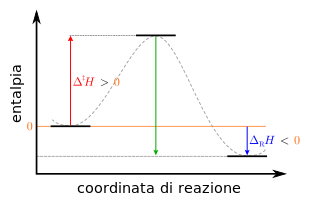
\includegraphics[scale=0.5]{bru}
\end{figure}
Dato il presente schema di reattività ci si dovrebbe aspettare che la reazione proceda spontaneamente, tuttavia data l'elevata barriera di attivazione essa risulta cineticamente inibita.
Dal punto di vista della termodinamica statistica questo tipo di reattività può essere visto come due stati termodinaci di equilibrio tra loro isolati; il primo dei due è quello collegato ai reagenti, infatti solo gli \emph{stati quantistici} che contemplano i reagenti separati saranno accessibili. Nel secondo stato termodinamico sia gli \emph{stati quantistici} dei reagenti separati, sia quelli dell'ammoniaca. 
Possiamo quindi definire due funzioni entropia, una per il primo stato termodinamico:
\begin{equation}
S=k\ln\Omega
\end{equation}
e una seconda  per il secondo:
\begin{equation}
S^\prime=k\ln\Omega^\prime
\end{equation}
Da questo punto di vista la differenza di entropia può essere riscritta come:
\begin{equation}
\Delta S=S^\prime-S=k\ln\frac{\Omega^\prime}{\Omega}
\end{equation}
Lo stato termodinamico dei prodotti contiene inevitabilmente più \emph{stati quantistici} rispetto a quello dei reagenti poiché  sono diventati accessibili anche i livelli energetici dell'ammoniaca. Quindi la molteplicità degli stati quantistici  $\Omega^\prime$ è maggiore della molteplicità degli stati quantistici $\Omega$. Da ciò possiamo dedurre che il rapporto tra le molteplicità sia sempre maggiore di $1$, di conseguenza il logaritmo sarà sempre positivo. Quindi:
\begin{equation}
\Delta S> 0
\end{equation}
Questa appena ottenuta è esattamente l'espressione della seconda legge della termodinamica che si ottiene classicamente.
\section{Sistemi di molecole indipendenti}
In un sistema di molecole indipendenti possiamo dividere i diversi contributi all'operatore hamiltoniano per molecole. Di conseguenza semplifichiamo un problema a molti corpi a tanti problemi a pochi corpi, dovendo di fatto risolvere l'equazione di  Schr\"{o}dinger per ogni singola molecola o sottosistema considerando quindi ogni molecola o sottosistema indipendente da quelli che lo circondano.
In questo modo si ottengono le singole energie che contribuiscono a quella dell'intero sistema.
\begin{equation}
\mathcal{H}_a\Psi_a=\epsilon_a\Psi_a
\end{equation}
Possiamo dunque immaginare di utilizzare questi valori dell'energia per costruire delle funzioni di partizione caratteristiche della molecola o del sottosistema selezionato. Per esempio si possono selezionare le funzioni d'onda vibrazionali dei singoli oscillatori e ottenere una funzione di partizione vibrazionale.
La domanda che sorge spontanea è: in che rapporto stanno queste funzioni di partizione con quella di tutto l'insieme?
La risposta può essere declinata in due casistiche:
\begin{itemize}
\item Particelle distinguibili: caso puramente teorico, in quanto realizzabile solo se tutte le molecole dell'insieme fossero diverse tra loro. La funzione di partizione totale è semplicemente:
\begin{equation}
Q=q^N
\end{equation}
nel caso in cui la distinguibilità sia stata aggiunta come condizione artificialmente a un insieme di molecole o sottosistemi identici. Altrimenti assume la seguente forma:
\begin{equation}
Q=\prod_a^N q_a
\end{equation}
\item Particelle indistinguibili: caso più aderente con la realtà in quanto si assume la presenza di molecole uguali tra loro nell'insieme. Questa assunzione aggiunge un grado di complicatezza. Analizziamo un semplice esempio per capire dove risiede questa nuova difficoltà.
Prendiamo un insieme molto semplice che contiene solo 3 molecole tra loro identiche e indipendenti. Generiamo ora $\mathcal{N}$ stati quantici, questi stati potranno essere permutati tra loro in $N!$ modi differenti. Di conseguenza gli stati quantici che sono generati per permutazione non dovrebbero essere contati nella funzione di partizione totale poiché equivalenti ad altri già inclusi. Per evitare questo problema si può dividire la moltiplicazione delle funzioni di partizione $q$ per il numero di permutazioni, contando così ogni permutazione singolarmente:
\begin{equation}
Q=\frac{q^N}{N!}
\end{equation}
Questa condizione si verifica esclusivamente nel caso in cui il numero di stati sia molto maggiore del numero di molecole o sottosistemi. Non è quindi più verificata per situazioni aderenti a statistiche di \emph{Bose-Eistein} o di 	\emph{Fermi-Dirac}.
\end{itemize}
Queste due riscritture della funzione di partizione totale in termini di quelle parziali possono essere utilizzate per ricavare le relazioni statistiche di energia totale e entropia utili per ottenere tutte le altre funzioni di stato termodinamiche, individuando così un collegamoento diretto tra mondo molecolare, o quantistico, e mondo macroscopico, o termodinamico.
Nel caso di particelle distinguibili:
\begin{equation}
\begin{aligned}
S&=kN\left[T\left(\frac{\partial\ln q}{\partial T}\right)_{V}+\ln q\right]\\
U&=NkT^2\left(\frac{\partial\ln q}{\partial T}\right)_{V}
\end{aligned}
\end{equation}
Mentre nel caso di particelle indistinguibili applicando l'approssimazione di \emph{Stirling }si ottiene:
\begin{equation}
\label{pioo}
\begin{aligned}
S&=kN\left[T\left(\frac{\partial\ln q}{\partial T}\right)_{V}+\ln q+\ln\frac{e}{N}\right]\\
U&=NkT^2\left(\frac{\partial\ln q}{\partial T}\right)_{V}
\end{aligned}
\end{equation}
\section{Variabili termodinamiche e funzioni di partizione}
Cosiderando la funzione di partizione dell'insieme canonico possiamo ricavare ora a partire dall'energia libera di Helmoltz (in quanto funzione caratteristica dell'insieme canonico) tutte le altre funzioni di stato:
\begin{equation}
\begin{aligned}
Q(N,V,T)&=\sum_je^{-\frac{E_j(N,V)}{kT}}\\
A(N,V,T)&=-kT\ln Q(N,V,T)\\
S&=-\left(\frac{\partial A}{\partial T}\right)_{V,N}=kT\left(\frac{\partial\ln Q}{\partial T}\right)_{V,N}+k\ln Q\\
p&=-\left(\frac{\partial A}{\partial V}\right)_{T,N}=kT\left(\frac{\partial\ln Q}{\partial T}\right)_{T,N}\\
U&=-T^2\left(\frac{\partial A/T}{\partial T}\right)_{V,N}=kT^2\left(\frac{\partial\ln Q}{\partial T}\right)_{V,N}\\
H&=U+pV=kT^2\left(\frac{\partial\ln Q}{\partial T}\right)_{V,N}+kVT\left(\frac{\partial\ln Q}{\partial T}\right)_{T,N}\\
G&=H-TS=-kT\ln Q+kVT\left(\frac{\partial\ln Q}{\partial T}\right)_{T,N}
\end{aligned}
\end{equation}
Nel paragrafo seguente sebbene ognuna di queste variabili possa essere derivata solo $U$ e $S$ verrano ricavate.
\section{Decomposizione della funzione di partizione molecolare}
Dato che è semplice scomporre un hamiltoniano molecolare nei suoi gradi di libertà, possiamo immaginare di scrivere una funzione di partizione molecolare in termini dei suoi contributi traslazionali, vibrazionali, rotazionali ed elettronici. Quindi la casistica delle particelle indipendenti indistinguibili diventa:
\begin{equation}
Q=\frac{(q_{tra}q_{rot}q_{vib}q_{el})^N}{N!}
\end{equation}
Andiamo ora ad analizzare i singoli contributi.
\subsection{Funzione di partizione traslazionale}
Per poter scrivere la funzione di partizione traslazionale di una singola molecola dobbiao prima calcolare l'energia traslazionale rifacendoci alla particella nella scatola:
\begin{equation}
\varepsilon_{n_x,n_y,n_z}=\frac{h^2(n_x^2+n_y^2+n_z^2)}{8ML^2}
\end{equation}
Questa espressione dell'energia va dunque inserita nella definizione di funzione di partizione estendendo la sommatoria a tutti i numeri quantici:
\begin{equation}
q_{tra}(V,T)=\sum_{n_x,n_y,n_z=1}^\infty e^\frac{-\varepsilon_{n_x,n_y,n_z}}{kT}
\end{equation}
Possiamo semplificare facendo variare i numeri quantici contemporaneamente e quindi sostituire i tre $n_j$ con un unico $n$.
\begin{equation}
q_{tra}(V,T)=\left[\sum_n^\infty \exp\left(-\frac{\varepsilon_n}{8kTLM^2}\right)\right]^3
\end{equation}
Questa sommatoria non può essere valutata analiticamente tuttavia dato che i termini successivi al primo sono tutti siili tra loro si può assumere che varino con continuità e trasformare la sommatoria in un integrale.
\begin{equation}
q_{tra}(V,T)=\left[	\int_0^\infty \exp\left(\frac{-h^2n^2}{8kTML^3}\right)dn\right]^3
\end{equation}
L'integrale è del tipo $\int e^{-an^2}dn=\left(\frac{\pi}{4a}\right)^{1/2}$ quindi la soluzione sarà:
\begin{equation}
\left[	\int_0^\infty \exp\left(\frac{-h^2n^2}{8kTML^3}\right)dn\right]^3=\left(\frac{2\pi MkT}{h^2}\right)^{3/2}V
\end{equation}
Possiamo ora sfruttare questa definizione della funzione di partizione molecolare traslazionale per derivare l'energia interna e l'entropia.
\begin{equation}
\begin{aligned}
U_{tra}&=NkT^2\left(\frac{\partial\ln q_{tra}}{\partial T}\right)_{V}=\frac{3}{2}NkT\\
S_{tra}&=kN\left[T\left(\frac{\partial\ln q_{tra}}{\partial T}\right)_{V}+\ln q+\ln\frac{e}{N}\right]\\
&=\frac{5}{2}Nk+Nk\ln\left[\left(\frac{2\pi MkT}{h^2}\right)_V^{3/2}\frac{V}{N}\right]
\end{aligned}
\end{equation}
\subsection{Funzione di partizione rotazionale}
Nel caso della funzione di partizione rotazionale ripetiamo concettualmente lo stesso procedimento adottato per quella traslazionale, inserendo nell'espressione della funzione di partizione l'equazione dell'energia rotazionale ricavata dalla meccanica quantistica.
\begin{equation}
\varepsilon_{J}=\frac{\hbar^2J(J+1)}{2I}
\end{equation}
Questa espressione dell'energia va dunque inserita nella definizione di funzione di partizione estendendo la sommatoria a tutti i livelli energetici e considerando la molteplicità di ogni livello energetico $2J+1$:
\begin{equation}
q_{rot}(T)=\sum_{J=0}^\infty(2J+1)e^\frac{-\hbar^2J(J+1)}{2kTI}
\end{equation}
Si può notare che tutte le costanti possono essere raccolte e tramite una non banale analisi dimensionale si giunge alla conclusione che esse abbiano complessivamente la dimensione di una temperatura, la \emph{temperatura rotazionale}. \index{temperatura rotazionale}
\begin{equation}
\theta_{rot}=\frac{\hbar^2}{2Ik}
\end{equation}
Svolgendo i calcoli si può dedurre l'entità di questa temperatura rotazionale, che se rapportata alle normali temperature operative risulta essere molto piccola. Dunque ogni membro della sommatoria contribuirà alla stessa in maniera irrisoria, si può quindi ripetere l'approssimazione della sommatoria a un integrale.
\begin{equation}
q_{rot}(T)=\int_{J=0}^\infty(2J+1)e^{\frac{-}{T}J(J+1)}dJ
\end{equation}
L'integrale è di semplice risoluzione in quanto basta operare la semplice sostituzione $x=J(J+1)$ ottenendo come risultato:
\begin{equation}
q_{rot}(T)=\frac{T}{\theta_{rot}}=\frac{8\pi^2IkT}{h^2}
\end{equation}
Le equazioni appena derivate sono valide solo per molecole eteroatomiche in quanto se si introducono atomi uguali entrano in gioco fattori di simmetria che costringono la funzione d'onda nucleare ad avere comportamento bosonico o fermionico a seconda dello spin nucleare. Nonostante ciò la formulazione della funzione di partizione non si complica eccessivamente:

\begin{equation}
q_{rot}(T)=\frac{T}{\sigma\theta_{rot}}
\end{equation}

Il fattore $\sigma$ che appare al denominatore, è il 	\emph{numero di simmetria}, ovvero un numero che indica quante orientazioni indipendenti ci siano nella molecola. Per esempio, in una molecola di acqua sarà 2, mentre in una di ammoniaca varrà 3.

Analoghe espressioni della funzione di partizione per rotatori con simmetrie diverse possono essere ricavate da una diversa impostazione della molteplicità.

Si riportano di seguito le espressioni per energia interna ed entropia per una molecola lineare:

\begin{equation}
\begin{aligned}
U_{rot}&=NkT\\
S_{rot}&=Nk(\ln q_{rot}+1)\\
\end{aligned}
\end{equation}

E per una non lineare:
\begin{equation}
\begin{aligned}
U_{rot}&=\frac{3}{2}NkT\\
S_{rot}&=Nk(\ln q_{rot}+\frac{3}{2})\\
\end{aligned}
\end{equation}
\subsection{Funzione di partizione vibrazionale}
In questo paragrafo l'approccio no cambia rispetto a quello adottato nei paragrafi precedenti. Quindi riscriviamo ora l'espressione dell'energia vibrazionale di una molecola e la inseriamo nella definizione di funzione di partizione.
\begin{equation}
t\varepsilon_n=\left(n+\frac{1}{2}\right) h\nu; \quad \nu =\frac{1}{2\pi}\sqrt[]{\frac{k}{\mu}}
\end{equation}
Con $k$ che è la costante elastica della molla e $\mu$ che è la massa ridotta del sistema. La funzione di partizione diventa dunque:
\begin{equation}
q_{vib}(T)=e^{-\frac{h\nu}{2kT}}\sum_{n=0}^\infty e^{-\frac{h\nu n}{kT}}
\end{equation}
La sommatoria può essere valutata facilmente se si condidera che converge a una serie geometrica:
\begin{equation}
\sum_{n=0}^\infty x^n=\frac{1}{1-x}
\end{equation}
Da cui deriva che:
\begin{equation}
q_{vib}(T)=\frac{e^{-\frac{\theta_{vib}}{2T}}}{1-e^{-\frac{\theta_{vib}}{T}}}
\end{equation}
In questa equazione introduciamo il concetto di \emph{temperatura vibrazionale}\index{temperatura vibrazionale} definita come:
\begin{equation}
\theta_{vib}=\frac{h\nu}{k}
\end{equation}
Anche in questo caso le relazioni termodinamiche possono essere dedotte applicando pedissequamente le equazioni riportate in \ref{pioo}. Non verranno riportate di seguito in quanto la derivazione è semplice ma il risultato complesso.
Nel caso in cui il sistema sia una molecola poliatomica, bisogna moltiplicare ogni funzione di partizione di ogni modo normale. La funzione di partizione totale diventa quindi:
\begin{equation}
q_{vib}(T)=\prod_{J=1}^\alpha\frac{e^{-\frac{\theta_{vib,J}}{2T}}}{1-e^{-\frac{\theta_{vib,J}}{T}}}
\end{equation}
Dove $J$ è un indice di modo normale, mentre $\alpha$ è il numero totale di modi normali.
\subsection{Funzione di partizione elettronica}
Nel caso di transizioni elettroniche, ha senso considerare solo i livelli che a temperature normali sono occupati. Quindi nella maggior parte dei casi solo i primi 2.
In particolare il primo livello per molecole monoatomiche in fase gas può essere preso 0, mentre in molcecole poliatomiche viene assunto pari al valore della buca di potenziale $D_e$.
\begin{equation}
q_{ele}(T)=g_1 e^{-\frac{\varepsilon_{ele,1}}{kT}}+g_2 e^{-\frac{\varepsilon_{ele,2}}{kT}}
\end{equation}
Se applicchiamo le approssimazioni che abbiamo definito all'inizio di questo paragrafo, si ottiene:
\begin{equation}
q_{ele}(T)=g_1 e^{-\frac{D_e}{kT}}+g_2 e^{-\frac{\varepsilon_{ele,2}}{kT}}
\end{equation}
Con $D_e=0$ nel caso di molecole monoatomiche.
Nel caso di molecole poliatomiche le relazioni termodinamiche diventano quindi:
\begin{equation}
\begin{aligned}
U_{ele}&=-ND_e\\
S_{ele}&=-\frac{ND_e}{T}+Nk\ln g_{ele,1}+\frac{ND_e}{T}\\
\end{aligned}
\end{equation}
\chapter{Applicazione della Termodinamica Statistica: Calcolo della dispersione fononica}
In questo capitolo verrà trattato un argomento spesso molto oscuro per gli studenti di Chimica, in quanto poco attinente con le conoscenze pregresse. Tuttavia i \emph{fononi} sono da cosiderarsi fondamentali nella caratterizzazione di un solido e nella sua definizione teorica più completa; è quindi di fondamentale importanza illustrare chiaramente le loro origini per poi giungere a una trattazione più formale.
\section{Fononi e vibrazioni reticolari}\index{fononi}\index{dispersione fononica}
Immaginamo un solido molecolare, ovvero un solido in cui tutte le posizioni reticolari siano occupate da una molecola. In un caso come questo, lo studio delle vibrazioni interne della molecola ci può portare alla definizione dello spettro vibrazionale della stessa. Tuttavia la molecola è ora vincolata all'occupazione di una posizione ben precisa a causa dell'energia potenziale dei suoi vicini. Ne consegue che i suoi tre gradi di libertà traslazionali in un solido tridimensionale vengono inibiti. Infatti essa potrà \emph{traslare} liberamente solo intorno a una posizione di equilibrio individuata da un minimo nella funzione \emph{energia potenziale della molecola}. Possiamo trattare la forma che assume questa energia potenziale con un'approssimazione armonica e scoprire che, di fatto, quelle che prima erano traslazioni ora sono vibrazioni o meglio oscillazioni intoerno a una posizione di equilibrio.
Questa condizione si verifica esclusivamente nel caso di un solido, pertanto è strettamente legata alla sua periodicità, infatti non possiamo analizzare una molecola isolata ignorando il resto del cristallo ma dobbiamo necessariamente razionalizzare le vibrazioni complessive di tutte le molecole che occupano posizioni reticolari in relazione con le altre.
Svolegere un simile calcolo significa andare a individuare quelli che per le vibrazioni molecolari vengono chimati \emph{modi normali} mentre nel nostro caso, delle vibrazioni reticolari verranno definiti \emph{fononi}.\index{fononi} Possiamo dunque iniziare a capire che i fononi hanno una diretta corrispondenza con i modi normali, ma a differenza di quest'ultimi essi non avranno necessariamente una frequenza unica. Infatti nel caso \emph{isotropico} si tende ad assumere che a ogni modo normale corrisponda necessariamente una frequenza. Tuttavia nei solidi a seconda della direzione lungo la quale si osseva un certo fenomeno esso può assumere connotazioni diverse. Questo è il caso dei fononi, infatti è possibile generare dei grafici che mostrano il variare della frequenza di una vibrazione reticolare a seconda della direzione in cui la si osserva. Con la direzione che viene definita da punti nello spazio reciproco, infatti a ogni punto dello spazio reciproco corrisponde una famiglia di piani nello spazio diretto e individuano dunque delle direzioni reticolari. Figure del tipo appena descritto vengono chiamate \emph{dispersioni fononiche}, un esempio è in figura \ref{fonodisp}.
\begin{figure}[H]
\centering
\caption{Dispersione fononica predetta e sperimentale sovrapposte per un solido semiconduttore}\label{fonodisp}
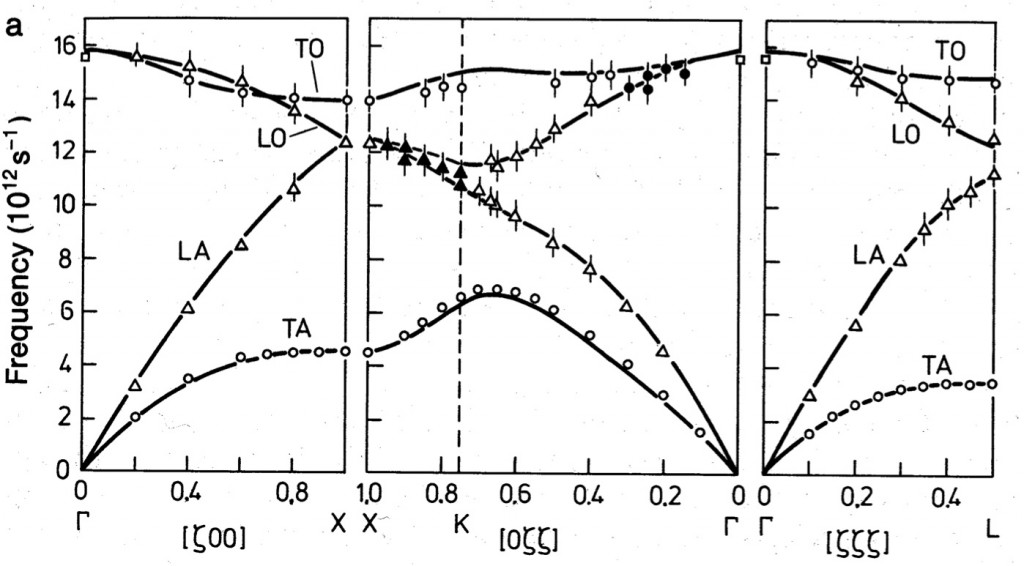
\includegraphics[scale=0.2]{fonodisp}
\end{figure}
Al fine di descrivere il fenomeno dei fononi sono stati sviluppati a inizio del XX secolo due modelli: il primo molto semplice di Einstein, e il secondo più complesso sviluppato da Debye. Ma prima di procedere con la descrizione di questi due modelli affronteremo la definizione formale del fenomeno.
\subsection{Descrizione matematica del fenomeno}
Immaginiamo di porre in ogni posizione reticolare di un reticolo monodimensionale una sfera collegata alle sue vicine mediante una molla come mostrato in figura \ref{molle}.
\begin{figure}[H]
\centering
\caption{Modello semplice a molle e sfere identiche tra loro per la descrizione delle vibrazioni reticolari.}\label{molle}
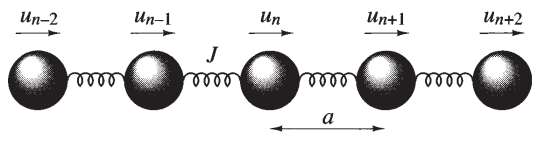
\includegraphics[scale=0.5]{molle}
\end{figure}
In questa situazione dobbiamo definire l'energia potenziale come l'energia a riposo sommata all'energia associata a uno spostamento lungo la catena monoatomica.
\begin{equation}
E=\underbrace{N\varphi}_\text{Energia a riposo di N atomi}+\underbrace{\sum_{s\geq1}\frac{1}{s!}\frac{\partial^2\varphi}{\partial u^2}\sum_n\left(u_n-u_{n+1}\right)^2}_{\text{Variazioni del potenziale dovute a vibrazioni}}
\end{equation}
Per semplificare i calcoli porremo a $0$ l'energia della catena a riposo e troncheremo l'espansione in serie di Taylor al secondo ordine, applicando quindi un'approssimazione armonica.
Si ottiene quindi:
\begin{equation}
E_{arm}=\frac{1}{2}J\sum_n\left(u_n-u_{n+1}\right)^2
\end{equation}
Dove $J$ è la derivata seconda dell'energia potenziale. Possiamo a questo punto inserire la definizione di energia appena ottenuta nella seconda legge della dinamica di Newton:
\begin{equation}
\label{fma}
m\frac{\partial^2u_n}{\partial t^2}=-\frac{\partial E_{arm}}{\partial u_n}=-J(2u_n-u_{n+1}-u_{n-1})
\end{equation}
Questa equazione appena ottenuta è un'equazione differenziale il cui risultato è:
\begin{equation}
u_n(t)=\sum_k \tilde{u}_k \exp (i[kx-\omega_kt])
\end{equation}
Inserendo questa definizione di $u_n$ in Eq. \ref{fma}, svolgendo la derivata e sostituendo $x=na$ è possibile ottenere la seguente equazione:
\begin{equation}
\begin{aligned}
&-m\omega_k^2\tilde{u}_k\exp(i[kna-\omega_kt])=\\&-J\tilde{u}_k\exp(-i\omega_kt)\left[2\exp(ikna)-\exp(ik[n-1]a)-\exp(ik[n+1]a)\right]
\end{aligned}
\end{equation}
Possiamo dunque isolare sia a destra che a sinistra dell'uguale le parti identiche e cancellarle:
\begin{equation}
\begin{aligned}
&-m\omega_k^2\tilde{u}_k\exp(i[kna-\omega_kt])=\\&-2J\tilde{u}_k\exp(i[kna-\omega_kt])\underbrace{\left[1-\frac{e^{ika}+e^{-ika}}{2}\right]}_{1-\cos ka}
\end{aligned}
\end{equation}
Cancellando  a destra e a sinistra dell'uguale e sostituendo il coseno si ottiene:
\begin{equation}
m\omega_k^2=2J(1-\cos ka)
\end{equation}
Per le formule di duplicazione possiamo convertire il coseno in seno infatti:
\begin{equation}
\begin{aligned}
\cos ka &= \cos2\alpha\\
\cos\alpha&=\cos^2\alpha-\sin^2\alpha\\
&=1-2\sin^2\alpha\\
&\text{Quindi:}\\
1-\cos ka&=2\sin^2\frac{ka}{2}
\end{aligned}
\end{equation}
Sostituendo ora nell'equazione semplificata e isolando a sinistra dell'uguale $\omega_k$ otteniamo:
\begin{equation}
\omega_k=\underbrace{\sqrt{\frac{4J}{m}}}_\textbf{A}\underbrace{\vert\sin(ka/2)\vert}_\textbf{B}
\end{equation}
Dove la parte \textbf{A} costituisce la soluzione classica delle frequenze di un modo normale di vibrazione mentre la parte \textbf{B} aggiunge una dipendenza periodica dal vettore d'onda $k$. Questo risultato ci può fare concludere che le vibrazioni reticolari non avranno sempre la stessa frequenza ma essa dipende dalle funzioni di Bloch che sono di fatto in grado di modulare la vibrazione reticolare. In un punto speciale $k=0$ detto $\Gamma$ la simmetria traslazionale delle funzioni di Bloch\index{Bloch !funzioni di} viene annulata e così il loro effetto di modulazione delle frequenze di vibrazione. Infatti in $\Gamma$ il cristallo non vibrerà in quanto il periodo di una singola funzione di Bloch risulta essere talmente grande che la vibrazione coinciderebbe di fatto con una traslazione dell'intero cristallo. Questo è il motivo per cui in $k=0$ le vibrazioni collettive del cristallo si annullano: perché degenerano in modi traslazionali.
A partire da questa equazione possiamo già costruire una prima approssimazione della figura di dispersione già citata in precedenza che assumerà la seguente forma:
\begin{figure}[H]
\centering
\caption{Semplice figura di dispersione.}\label{acu}
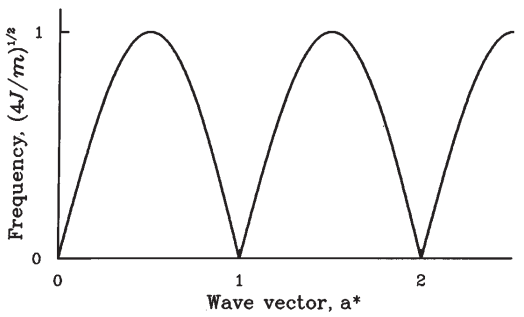
\includegraphics[scale=0.5]{acu}
\end{figure}
Osservando la figura \ref{acu} si nota che tutta l'informazione sulla dispersione è racchiusa tra $0$ e $a^*/2$ ovvero nella prima zona di Brillouin, infatti sarà sufficiente esplorare i punti ad elevata simmetria in questa zona per avere un'idea di come si comporterà la funzione nel resto del reticolo reciproco. 
\subsection{Cristalli di atomici:formalismo matematico}
Un modello un po' più complicato ma sicuramente più descrittivo della realtà assume che possano esserci atomi con masse diverse e costanti di forza delle molle che dipendono da quali atomi ci siano legati. Un modello semplice monodimensionale può aiutarci a descrivere matematicamente anche questa situazione.
\begin{figure}[H]
\centering
\caption{Catena lineare diatomica.}\label{AA1}
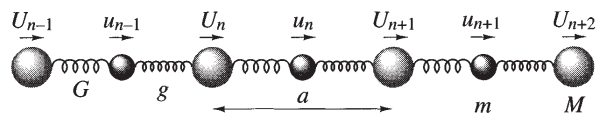
\includegraphics[scale=0.5]{AA1}
\end{figure}
In questo caso le costanti elastiche sono rappresentate da g e G mentre le masse da m e M. L'impostazione del problema è la stessa adottata per la catena monoatomica, ma in questo caso si otterrà un sistema di 2 equazioni, una per la massa piccola e una per quella grande.
\begin{equation}
\begin{aligned}
-M\omega^2_k\tilde{U}_k&=-(G+g)\tilde{U}_k+(G+g\exp(-ika))\tilde{u}_k\\-m\omega^2_k\tilde{u}_k&=-(G+g)\tilde{u}_k+(G+g\exp(-ika))\tilde{U}_k
\end{aligned}
\end{equation}
Il sistema può essere facilmente risolto ponendo a zero il determinante della matrice collegata alle equazioni. Il risultato che si ottiene alla fine è il seguente:
\begin{equation}
\omega^2_k=\frac{(M+m)(G+g)}{2Mm}\pm\frac{\left((M+m)^2(G+g)^2-16mMgG\sin^2ka/2)\right)^{1/2}}{2Mm}
\end{equation}
Le cui due soluzioni al limite $k\rightarrow0$ si riducono a:
\begin{equation}
\begin{aligned}
\omega^2_{k1}&=\frac{(M+m)(G+g)}{Mm}-O(k^2)\\
\omega^2_{k2}&=\frac{Ggk^2a^2}{(M+m)(G+g)}
\end{aligned}
\end{equation}
Le due soluzioni posso qindi essere rappresentate in forma grafica generando la figura \ref{AA2}:
\begin{figure}[H]
\centering
\caption{Soluzioni della catena lineare diatomica.}\label{AA2}
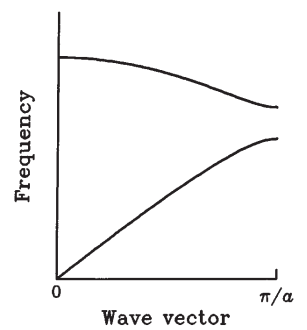
\includegraphics[scale=0.5]{AA2}
\end{figure}
I due rami che si vedono in figura \ref{AA2} in base alle frequenze che esplorano prendono due nomi diversi:
\begin{itemize}
\item \textbf{Ramo acustico}\index{Ramo acustico} Si trova a frequenze basse ed è associato a vibrazioni a bassa energia, la velocità di propagazione di questi modi coincide con la velocità del suono nel solido. Questi modi vengono eccitati mediante semplici sollecitazioni meccaniche del solido.
\item \textbf{Ramo ottico}: \index{Ramo ottico}Occupa una zona di frequenze tipica della radiazione elettromagnetica. Ha sempre valori positivi diversi da $0$. L'eccitazione dei modi ottici avviene esclusivamente per interazione radiazione-materia.
\end{itemize}
Risulta essere importante fare un breve ragionamento sulla lunghezza d'onda collegata a questi modi di vibrazione. Infatti essa è la lunghezza d'onda della funzione di Bloch che modula la vibrazione, è quindi evidente la differenza tra i modi acustici e i modi ottici. Infatti i primi saranno caratterizzati da una lunghezza d'onda maggiore del parametro reticolare, quindi la vibrazione avviene tra celle diverse. Mentre la lunghezza d'onda dei modi ottici può essere più piccola del parametro reticolare coinvolgendo anche vibrazioni molecolari. Questo risultato lo si ottiene matematicamente inserendo le soluzioni per $\omega_k^2$ nell'equazione matriciale al limite $k=0$. Infatti per i modi acustici si scopre che tutti gli spostamenti atomici sono in fase:
\begin{equation}
\tilde{U}_0=\tilde{u}_0
\end{equation}
Mentre per i modi ottici gli spostamenti saranno fuori fase, quindi in grado di generare dipoli sfruttabili da una radiazione elettromagnetica per attivare la vibrazione.
\begin{equation}
M\tilde{U}_0=-m\tilde{u}_0
\end{equation}
Queste soluzioni si applicano esclusivamente al caso in cui le vibrazioni siano valutate in $\Gamma$.
\subsection{Comportamento al confine della FBZ}
Ai confini della FBZ entrambi i rami hanno curvatura nulla solo in casi ad elevata simmetria, infatti se il vettore d'onda non è perpendicolare al confine della FBZ solo la componente normale avrà curvatura nulla.
Un'importante eccezione a queste condizioni di curvatura è costituita dal caso in cui sia presente un'asse di simmetria elicoidale o uno slittopiano. Infatti la pendenza del ramo superiore è l'opposto di quella del ramo inferiore generando di fatto un ripiegamento del ramo come si può vedere in figura \ref{AA3}.

\begin{figure}[H]
\centering
\caption{Soluzioni della catena lineare diatomica.}\label{AA3}
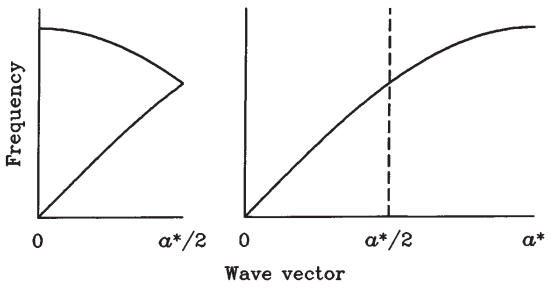
\includegraphics[scale=0.5]{AA3}
\end{figure}

La presenza degli operatori di simmetria spaziale citati sopra implica l'espansione della cella fondamentale con conseguente rimpicciolimento della prima zona di Brillouin. Se la FBZ si rimpicciolisce quindi le bande fononiche vengono ripiegate affinché rientrino nella FBZ.
\section{Il modello di Einstein}\index{Einstein !modello di}
Il modello di Einstein costituisce il primo e più semplice modello che è stato sviluppato per correlare delle grandezze termodinamiche alla teoria dei fononi utilizzando la termodinamica statistica. Questo modello è basato su alcune assunzioni:
\begin{itemize}
\item Ogni vibrazione è indipendente da quelle vicine;
\item Il potenziale a cui è sottoposta una molecola che vibra è perfettamente sferico;
\item Tutte le vibrazioni avvengono a una sola frequenza, ovvero la distribuzione delle frequenze è una delta di Dirac.
\end{itemize}
Un esempio di distribuzione a delta di Dirac è mostrato in figura \ref{AA4}.
Per definire un collegamento tra termodinamica statistica e fononi dobbiamo in primo luogo decidere quale sia l'entità chimica di cui considereremo l'ensemble. Per quanto riguarda i fononi è logico prendere come entità chimica la singola vibrazione definita da un modo normale e da una frequenza.
\begin{figure}
\centering
\caption{Distribuzione delle frequenze nel modello di Einstein.}\label{AA4}
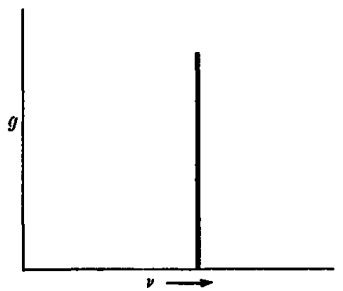
\includegraphics[scale=0.5]{dirac}
\end{figure}
Dato che tutti gli oscillatori vibrano alla stessa frequenza allora possiamo dedurre che basti moltiplicare la funzione di partizione di un oscillatore per il numero di oscillatori quindi:
\begin{equation}
Q=e^{-N\varphi(0)/2kT}q^{3N} 
\end{equation}
Il termine esponenziale che precede la funzione di partizione serve a impostare uno zero del potenziale, infatti esso contiene il valore centrale del potenziale. In questo modo si evita di contare più volte diverse interazioni molecolari. 
Deriviamo ora la funzione di partizione vibrazionale, a partire dalla definizione di energia vibrazionale.
\begin{equation}
\begin{aligned}
q&=\sum_{n=0}^\infty e^{-\varepsilon_n/kT}\\
\varepsilon_n&=\left(n+\frac{1}{2}\right)h\nu\\
q&=e^{-h\nu/2kT}\underbrace{\sum_{n=0}^\infty e^{-hn\nu/kT}}_{\frac{1}{1-e^{-h\nu/kT}}}\\
&=\frac{e^{-h\nu/2kT}}{1-e^{-h\nu/kT}}=\frac{e^{-\Theta/2T}}{1-e^{-\Theta/T}}
\end{aligned}
\end{equation}
Dove $\Theta=h\nu/k$ e ha le dimensioni di una temperatura che tipicamente vale $300K$.
Ora proviamo a derivare la \emph{capacità termica} che può essere confrontata facilmente con valori sperimentali in modo da validare o meno il modello di Einstein.\index{capacità termica}
\begin{equation}
\begin{aligned}
E&=kT^2\left(\frac{\partial \ln Q}{\partial T}\right)_{N,V};\\
C_v&=\left(\frac{\partial E}{\partial T}\right)_{N,V}=3Nk\left(\frac{\Theta}{T}\right)^2\frac{e^{\Theta/T}}{(e^{\Theta/T}-1)^2}
\end{aligned}
\end{equation}
Questa legge, sebbene $V/N$ cambi per un singolo cristallo e $\Theta$ è caratteristico di ogni cristallo, può essere resa generale operando trasformazioni dei dati sperimentali. Tuttavia se si confrontano le curve sperimentali con i valori predetti dal modello di Einstein si nota che essi non coincidono. Ne deduciamo che le approssimazioni applicate siano troppo drastiche e quindi si debba aggiungere un po' di complessità al modello per ottenere un migliore accore sperimentale.
\section{Il modello di Debye}\index{Debye !modello di}
Nel modello di Debye viene meno la più grande approssimazione fatta nel modello di Einstein, ovvero la distribuzione delle frequenze a delta di Dirac. Infatti in questo modello si assume che le frequenze abbiano una distribuzione e che questa distribuzione abbia un comportamento asintotico a 0 per frequenze basse, come mostrato in figura \ref{AA5}.
\begin{figure}
\centering
\caption{Distribuzione delle frequenze nel modello di Debye}\label{AA5}
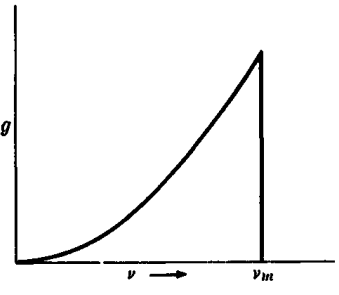
\includegraphics[scale=0.5]{AA5}
\end{figure}
Dato che la distribuzione è un continuo allora una simile approssimazione considera anche le frequenze come un continuo e ciò è valido solo per frequenze basse per cui la lunghezza d'onda sia superiore al parametro di cella, ovvero per i modi acustici.
Dato che la funzione di partizione è troppo complicata da ricavare, riportiamo qui direttamente il suo logaritmo:
\begin{equation}
\ln Q=-\frac{N\varphi(0)}{2kT}-\int_0^\infty\left[\ln(1-\exp(-h\nu/kT))+\frac{h\nu}{2kT}\right]g(\nu)d\nu
\end{equation}
Sfruttando la definizione di energia possiamo ricavarci anche la capacità termica:
\begin{equation}
C_v=3Nk\left[4D(u)-\frac{3u}{e^u-1}\right];\quad u=\frac{\Theta_D}{T}
\end{equation}
In questa equazione $D$ è una funzione che viene valutata numericamente.
Il comportamento del modello di Debye nei confronti dei dati sperimentali è decisamente migliore di quello di Einstein, infatti esso prevede correttamente l'andamento in ogni range di temperatura. Tuttavia se sottoposta a test più sensibili questa teoria risulta nuovamente incompleta. Sia il modello di Eistein che quello di Debye sono stati derivati in un periodo storico privo di metodi computazionali, pertanto è logico che non si potessero costruire modelli troppo complicati. Nonostante ciò essi costituiscono dei perfetti esempi di modelli semplici in grando di spiegare qualitativamente il fenomeno fisico.
\newpage
\printindex
\chapter*{Ringraziamenti}
Quest'opera è costituita in molte sue parti da una traduzione e rivisitazione del testo \emph{Introduction to Computational Chemistry} di \emph{Frank Jensen} edito da \emph{Wiley}. La parte di Termodinamica Statistica è basata principalmente sull'edizione italiana di \emph{Introduzione alla Termodinamica statistica} edita da \emph{PICCIN} e sugli appunti del corso di Complements of Computational Material Science della professoressa A.M. Ferrari. Altre parti, così come l'organizzazione generale del testo sono tratte dalle dispense del corso di Chimica Computazionale redatte dai docenti B. Civalleri e C. Roetti. L'idea dietro questo testo è di integrare le dispense del corso con approfondimenti tratti dal libro di testo e con gli appunti presi a lezione dall'autore. Si ringrazia per la revisione scientifica il collega G. Deplano e, per il sostegno morale, la mia compagna M. Cavallo.
Un ringraziamento speciale va al mio relatore R. Dovesi senza il quale non avrei ottenuto le competenze informatiche necessarie sia a redigere questo documento, sia alla comprensione profonda di una buona parte degli argomenti trattati nel corso di Chimica Computazionale.
\newpage
\end{document}
